% arara: lualatex: { shell: yes, action: nonstopmode, synctex: yes}
% arara: lualatex: { shell: yes, action: nonstopmode, synctex: yes}
\documentclass[landscape]{article}
\usepackage[ngerman]{babel}
\usepackage[no-math]{fontspec}

\usepackage{mwe}
\usepackage{luacode}
\usepackage{shellesc}
% \documentclassw[11pt, a4paper,ngerman]{article}
\usepackage{basicff}
\usepackage{sectsty}
\usepackage{adjustbox} % minipage top allign
\usepackage{subfigure} % Bilder nebeneinander darstellen

\usetikzlibrary{patterns} % preamble
\tcbuselibrary{skins} % preamble

\usepackage{tikz}
% \usepackage{PTSansNarrow}
\usetikzlibrary{matrix}

\usepackage{pgfplots}
\pgfplotsset{
 compat=newest
  }
\tcbset{colframe=red!75!black}
\newenvironment{proggen}{\begin{center}}{\end{center}}

\usepackage{array}
% \setmainfont[Path=/Applications/Microsoft Word.app/Contents/Resources/Fonts/]{Calibri.ttf}
% \setsansfont[Path=/Applications/Microsoft Word.app/Contents/Resources/Fonts/]{Calibri.ttf}
% \setmonofont[Path=/Applications/Microsoft Word.app/Contents/Resources/Fonts/]{Calibri.ttf}
% \usepackage{datetime}
% \pagestyle{fancy}


\setmainfont{UbuntuL.ttf}
\setsansfont{UbuntuR.ttf}
\setmonofont{UbuntuMonoR.ttf}

\newcolumntype{C}[1]{>{\centering\arraybackslash}m{#1}}

\oddsidemargin-10mm
\title{
\color{white}
\begin{center}
 \includegraphics[scale=1.0]{./pictures/NoPLogo.png}
\end{center}
 $\bullet$ \\
 % $\bullet$ \\ $\bullet$ \\
 \color{black}
 % \color{white}
 % $\bullet$ \\
 \color{black}
 TeX-Dokumente automatisiert \\mit \\GitHub und Travis-CI \\bauen \\
\color{white}
$\bullet$ \\
\color{black}
%  \begin{center}
% 	\includegraphics[scale=0.5]{./pictures/NoPLogo.png}
% \end{center}
 % \includegraphics{./pictures/wohnzimmer.png}
}
% \includegraphics{./pictures/asrock.png} Q1900M \\ \color{white} $\bullet$ \\ $\bullet$ \\ $\bullet$ \\ \color{black} \\ \apple \\ 10.10.3

\author{Daniel Krah}
% \rfoot{Compiled on \today\ at \currenttime}
% \cfoot{}
% \lfoot{Page \thepage}
% \date{1.6.2015}

\begin{document}
\huge


\sectionfont{\Huge}
\subsectionfont{\Huge}
\subsubsectionfont{\Huge}
\paragraphfont{\Huge}


\AddToShipoutPicture{\BackgroundPic}
\maketitle%
% \newpage%
 % \tableofcontents%
% \newpage
%==================================================================================
% \begin{center}
% \textbf{Vorwort}
% \end{center}



%
% \input{hardware.tex}



% \begin{itemize}
% \item test
% \item Deine Mudda
% \end{itemize}
%
% gh

%  To Do
% \input{todo.tex}
\newpage
% \section{Überblick}


% \begin{displaymath}
%   E = \frac{m_{0} c^{2}}{\sqrt{1-v^{2}/c^{2}}}
% \end{displaymath}

% \begin{luacode}
%   for x=1,600 do
%     tex.print(x+2)
%   end
% \end{luacode}
\section{Warum \LaTeX \  bzw. LUA\TeX ?}
\subsection{Vorteile von \LaTeX}
\begin{itemize}
  \item Tex Dateien kann man auch noch nach Jahren öffnen \\und in der Regel auch übersetzen.
  \item Keine Binärdateien. (Dokument auf Github direkt lesbar)
  \item Einfaches zusammenarbeiten (merge problemlos möglich)
  \item Nutzung mit Github und Travis CI relativ einfach
\end{itemize}
\subsection{Warum dann LUA\TeX ?}
\begin{itemize}
  \item Unterstützung von True-Type-Schriften \\(KEIN Zugriff auf Systemschriften !!!)
  \item komplexeres Programmieren innerhalb von Tex möglich.
\end{itemize}


\section{Warum GitHub und Travis-CI ?}

Im Prinzip könnte man jeden x beliebigen Server ... \\
Dort: \\
ein Git Repo + ssh und ein CI System. \\

Man könnte eines selbst zu Hause hosten und hätte die volle Kontrolle.\\

ABER:
Als Student möchte man vielleicht in Gruppen zusammen arbeiten um sich zusammen eine Mitschrift anzufertigen.
Nicht jeder möchte sich eine komplette \LaTeX - Installation an tun.\\

\"{}Och ne, iss mir zuviel Uffriss ...\"{} \\

Durfte ich mir schon oft anhören.






% \begin{itemize}
%   \item Tex Dateien kann man auch noch nach Jahren öffnen \\und in der Regel auch übersetzen.
%   \item Keine Binärdateien. (Dokument auf Github direkt lesbar)
%   \item Einfaches zusammenarbeiten (merge problemlos möglich)
%   \item Nutzung mit Github und Travis CI relativ einfach
% \end{itemize}
% \subsection{Warum dann LUA\TeX ?}
% \begin{itemize}
%   \item Unterstützung von True-Type-Schriften \\(KEIN Zugriff auf Systemschriften !!!)
%   \item komplexeres Programmieren innerhalb von Tex möglich.
% \end{itemize}
  %  Warum Latex

\newpage

\section{Github + Travis CI - \ \  \"{} the pdflatex way \"{}}
\subsection{Was wird benötigt ?}
{\color{green}Kostenlose} Variante (nur public Repo's):
\begin{itemize}
  \item Ein Github - Account
  \item Ein Travis-CI (.org) Account
  \item Das Travis Command-line Tool
\end{itemize}
\vspace{0.5cm}
{\color{red}Kostenpflichtige} / Studenten Variante \\(Auch private Repo's / und sofortige build's):
\begin{itemize}
  \item Ein kostenpflichtiger Github - Account ( \$7/ Monat)
  \item Ein kostenpflichtiger Travis-CI (.com) Account ( \$69/ Monat)
  \item Alternativ ein Student Developer Pack von Github \\ siehe: https://education.github.com/pack
  \item Das Travis Command-line Tool
\end{itemize}


%
%   Seite 4
%
%   Github
%
\newpage
\subsection{Einrichtung}
\subsection{Github}
Als erstes benötigen wir einen Github Account inkl. Repo.
\begin{center}
  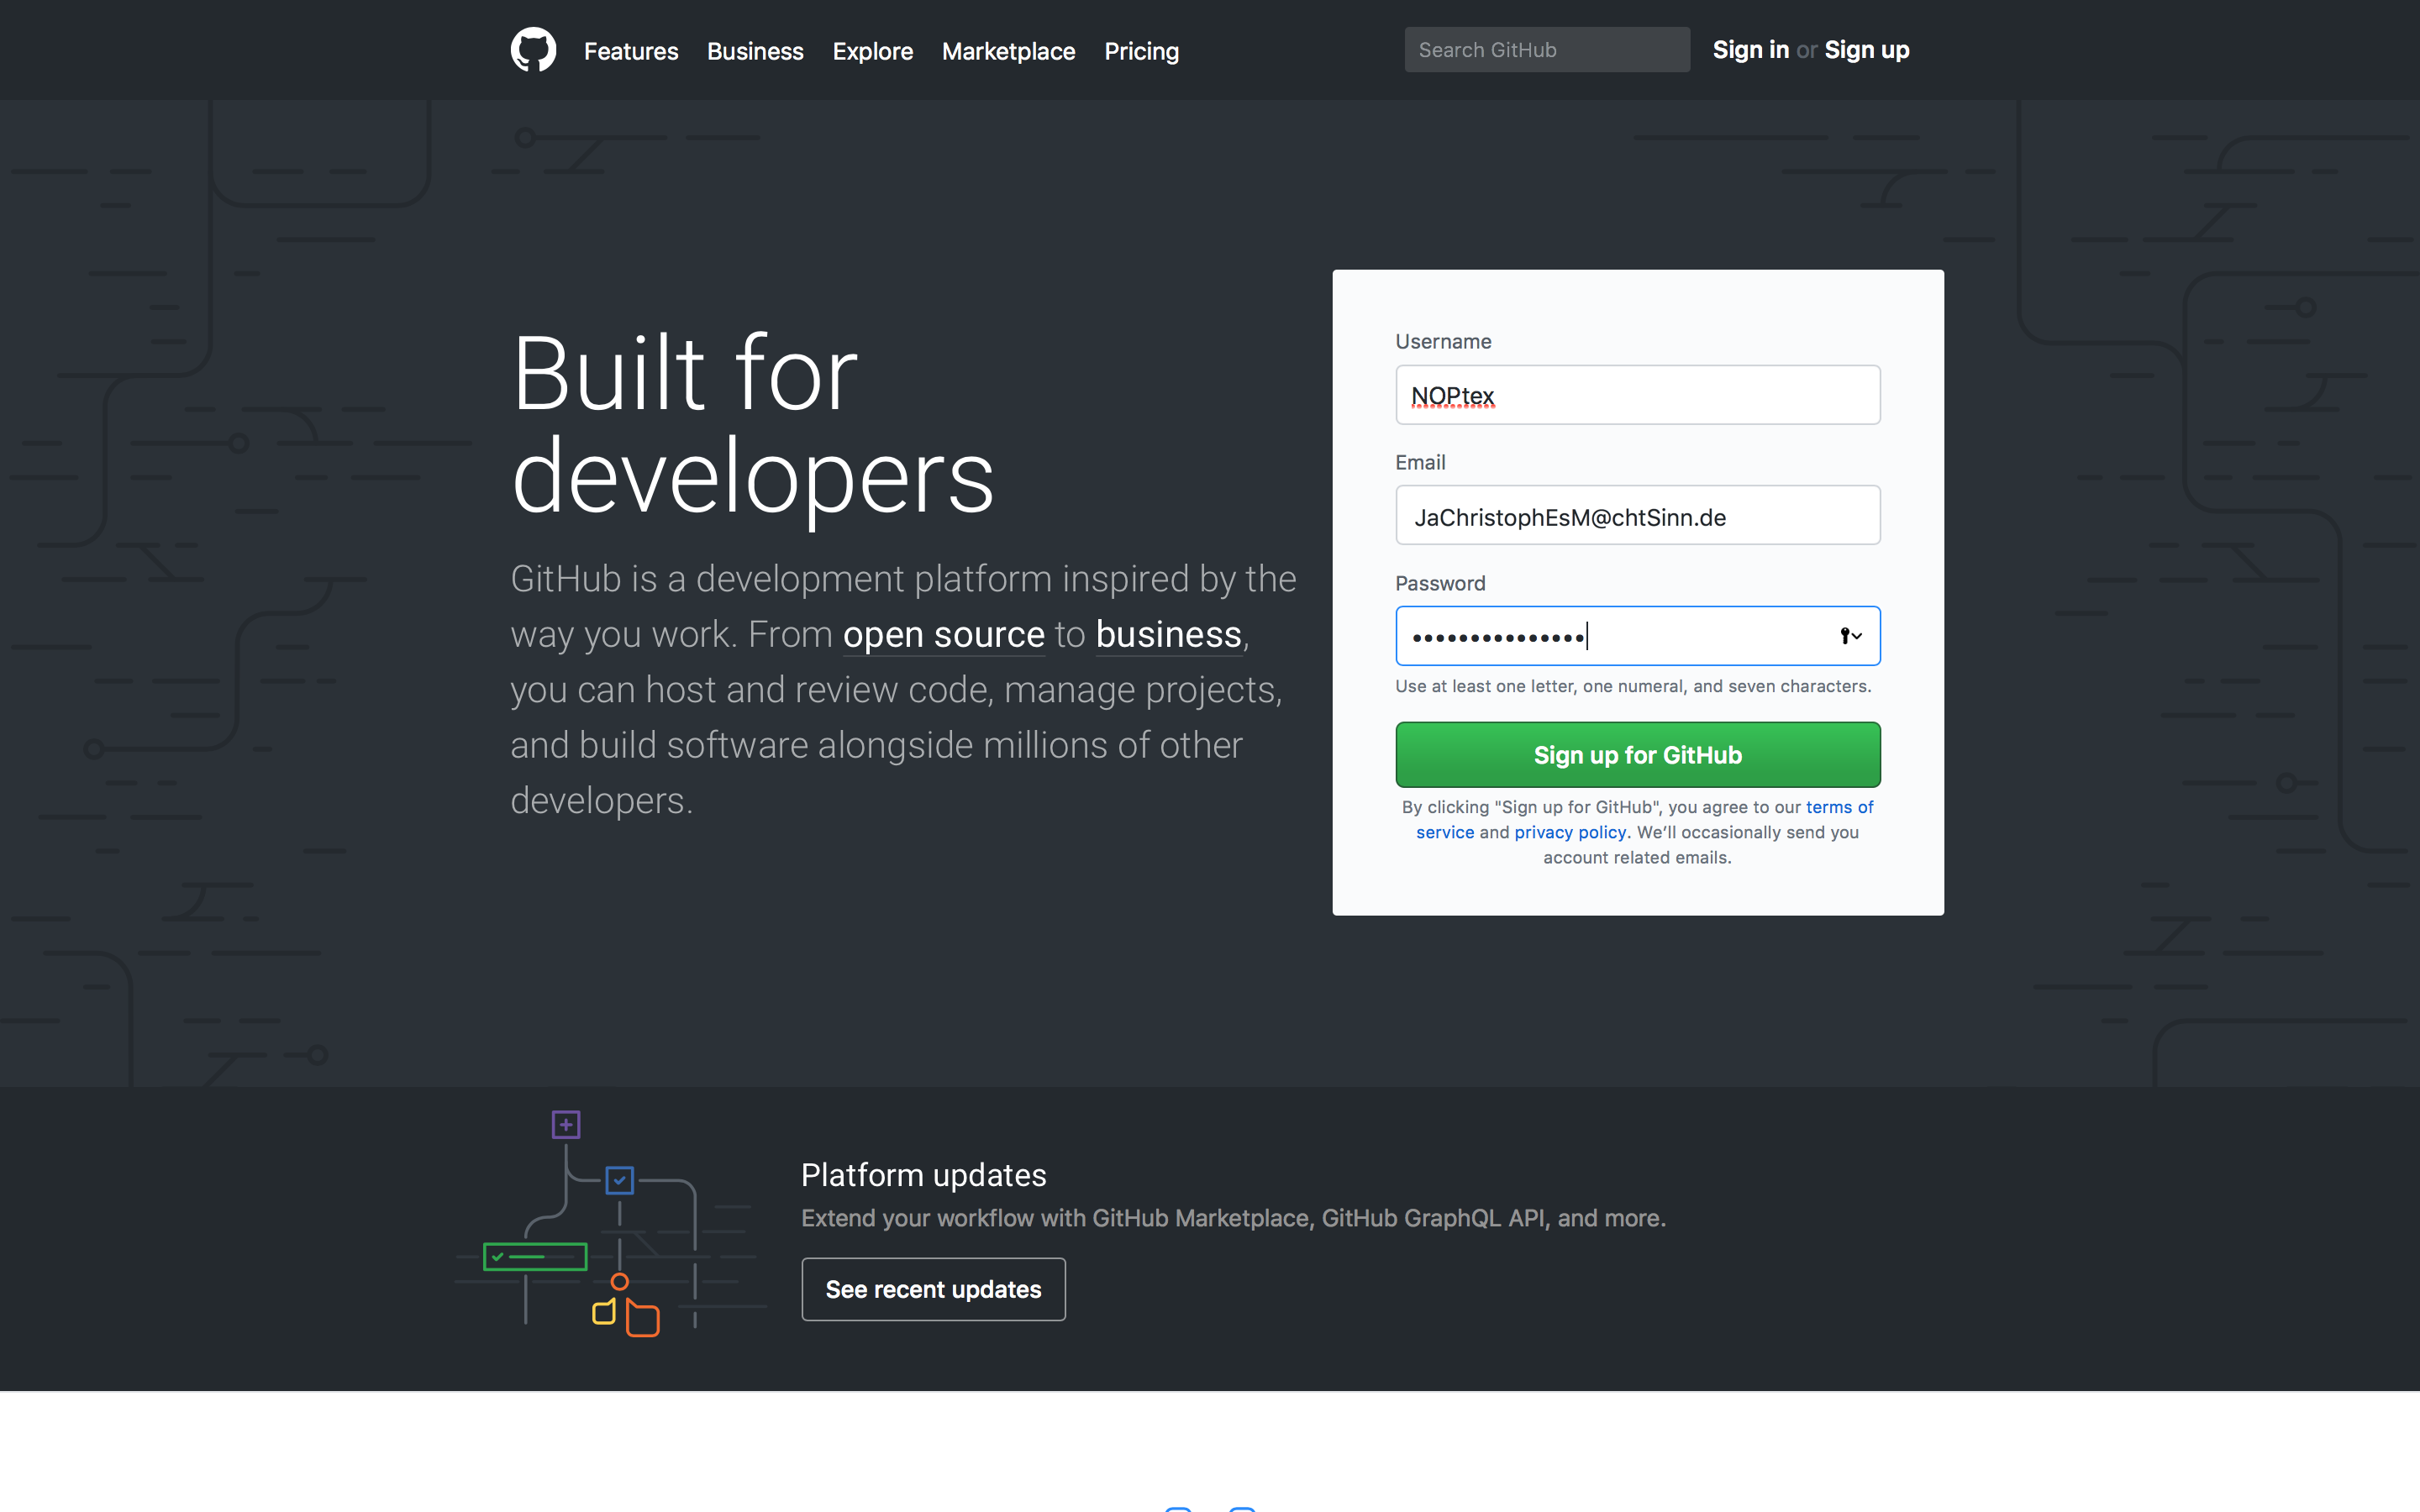
\includegraphics[trim = 300px 10px 300px 0px, clip,height=11cm]{./bilder/1Github.png}
\end{center}

% "l, b, r, t"
% \begin{figure}
% 	\centering
% \end{figure}\includegraphics[trim = 20px 10px 20px 30px, clip, width=\textwidth]{Beispiel.jpg}
% 	\caption{Hier steht der Beschriftungstext.}
% 	\label{fig:Beispiel}
% \end{figure}



\newpage
(Im Verlauf dieses Vortrages verwende ich:\\

https://github.com/NOPtex/NOP)\\


Dort befindet sich ein funktionierender Prototyp. \\
(Welcher aber noch ein paar zusätzlich Dateien beinhaltet.) \\

Prinzipiell reicht eine \TeX -Datei und die .travis.yml.

\begin{center}
  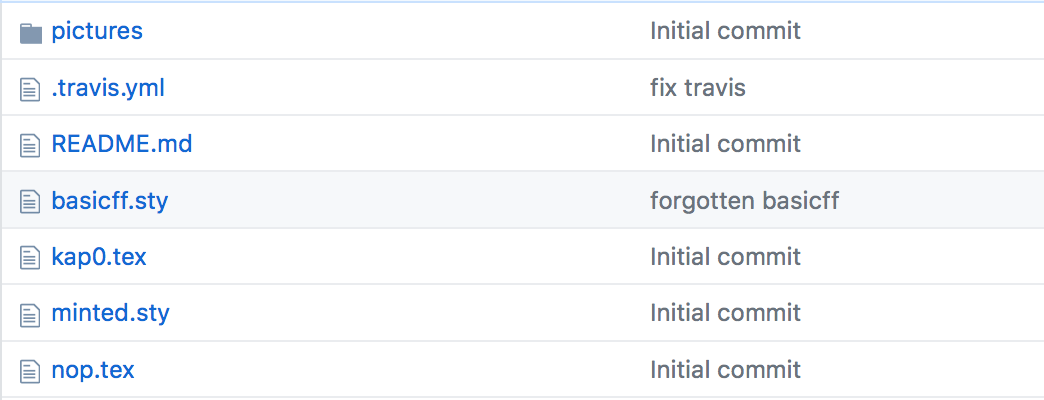
\includegraphics[width=0.8\textwidth]{./bilder/2Boilerplate.png}
\end{center}

%
%
% \vspace{0.5cm}
%
% \begin{center}
%   \includegraphics[width=1.0\textwidth]{./bilder/plainRepo.png}
% \end{center}

%
%   Seite 5
%
%   Github
% \cleardoublepage

\newpage % ============================================= Newpage ===================


\begin{figure}[ht]
  \subsection{Travis CI}
  \subsubsection{In Travis CI einloggen und mit Github verbinden}
\adjustbox{valign=t}{\begin{minipage}[t]{0.50\textwidth}
\begin{framed}
  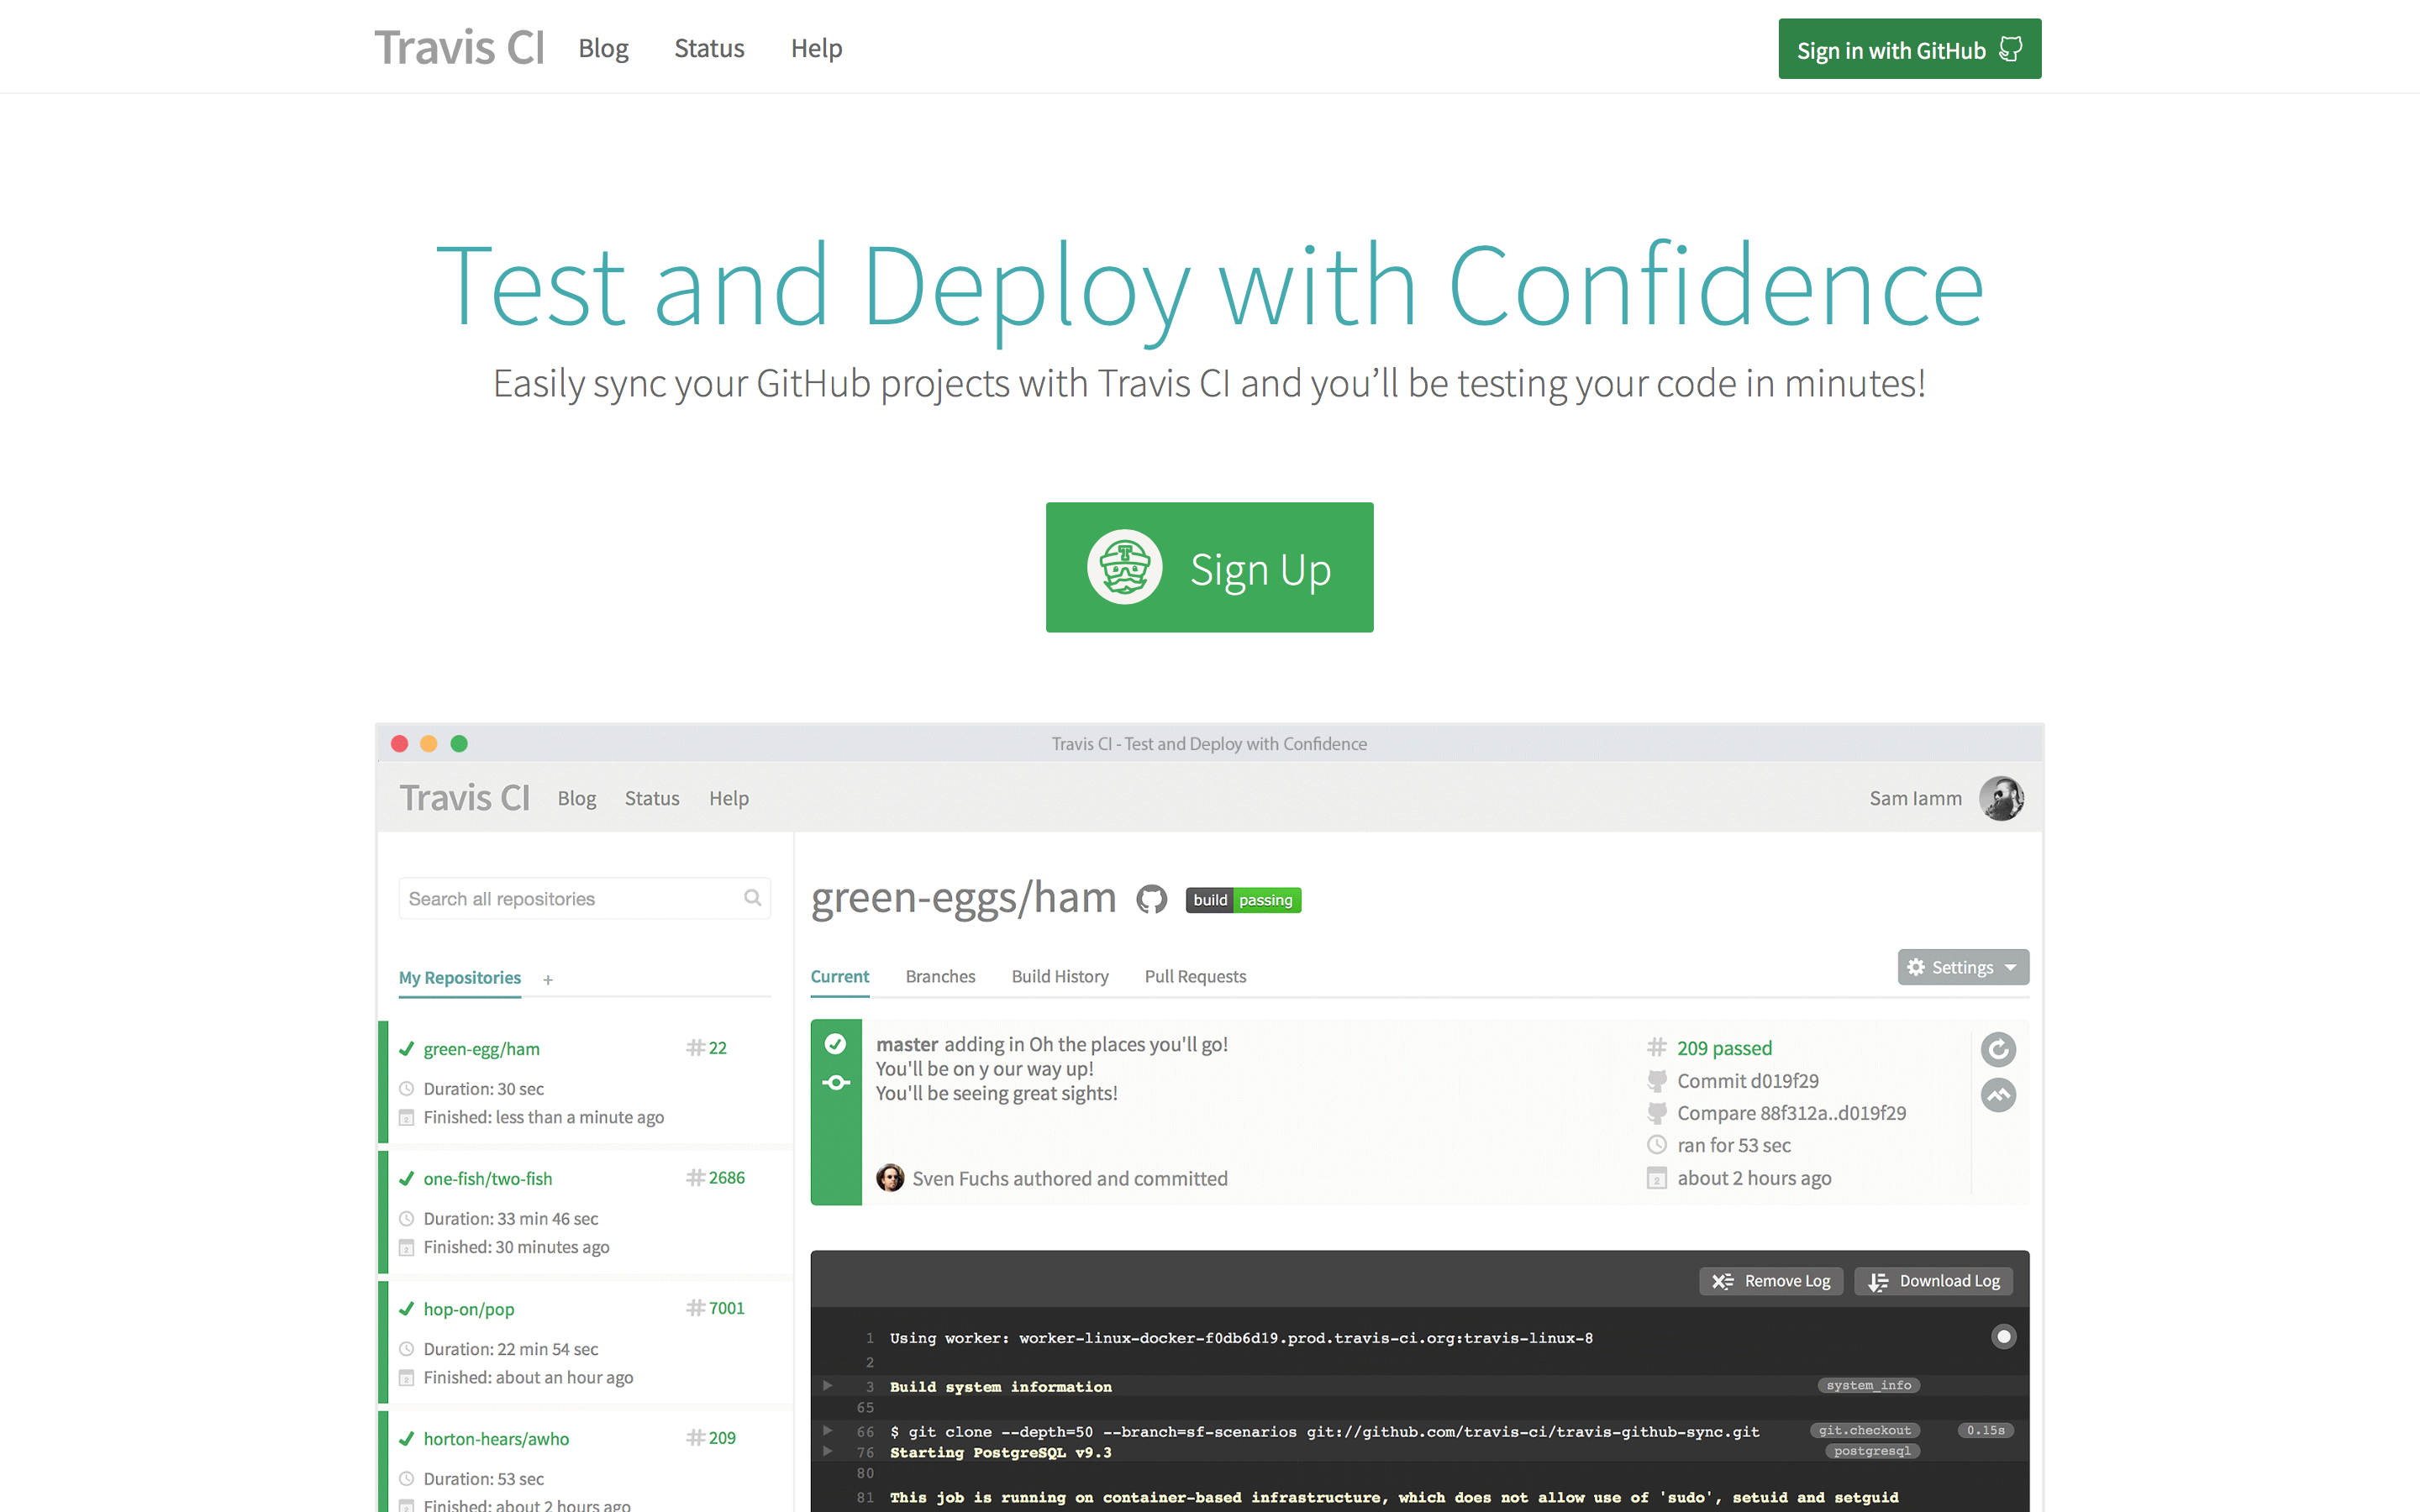
\includegraphics[width=1.0\textwidth]{./bilder/3travisSignUP.png}
\end{framed}

\end{minipage}}
% \hfill
\adjustbox{valign=t}{\begin{minipage}[t]{0.45\textwidth}
\vspace{0pt}
\huge
Da Travis nur mit Github \\funktioniert ist die Einrichtung recht \"{}trivial\"{}.
% \caption{Kapazität}
\end{minipage}}
% \end{figure}
% \vspace{0.5cm} % ----------------------------------- vspace
% \begin{figure}[ht]
\adjustbox{valign=t}{\begin{minipage}[t]{0.50\textwidth}
% \vspace{0.5cm}
\begin{framed}
  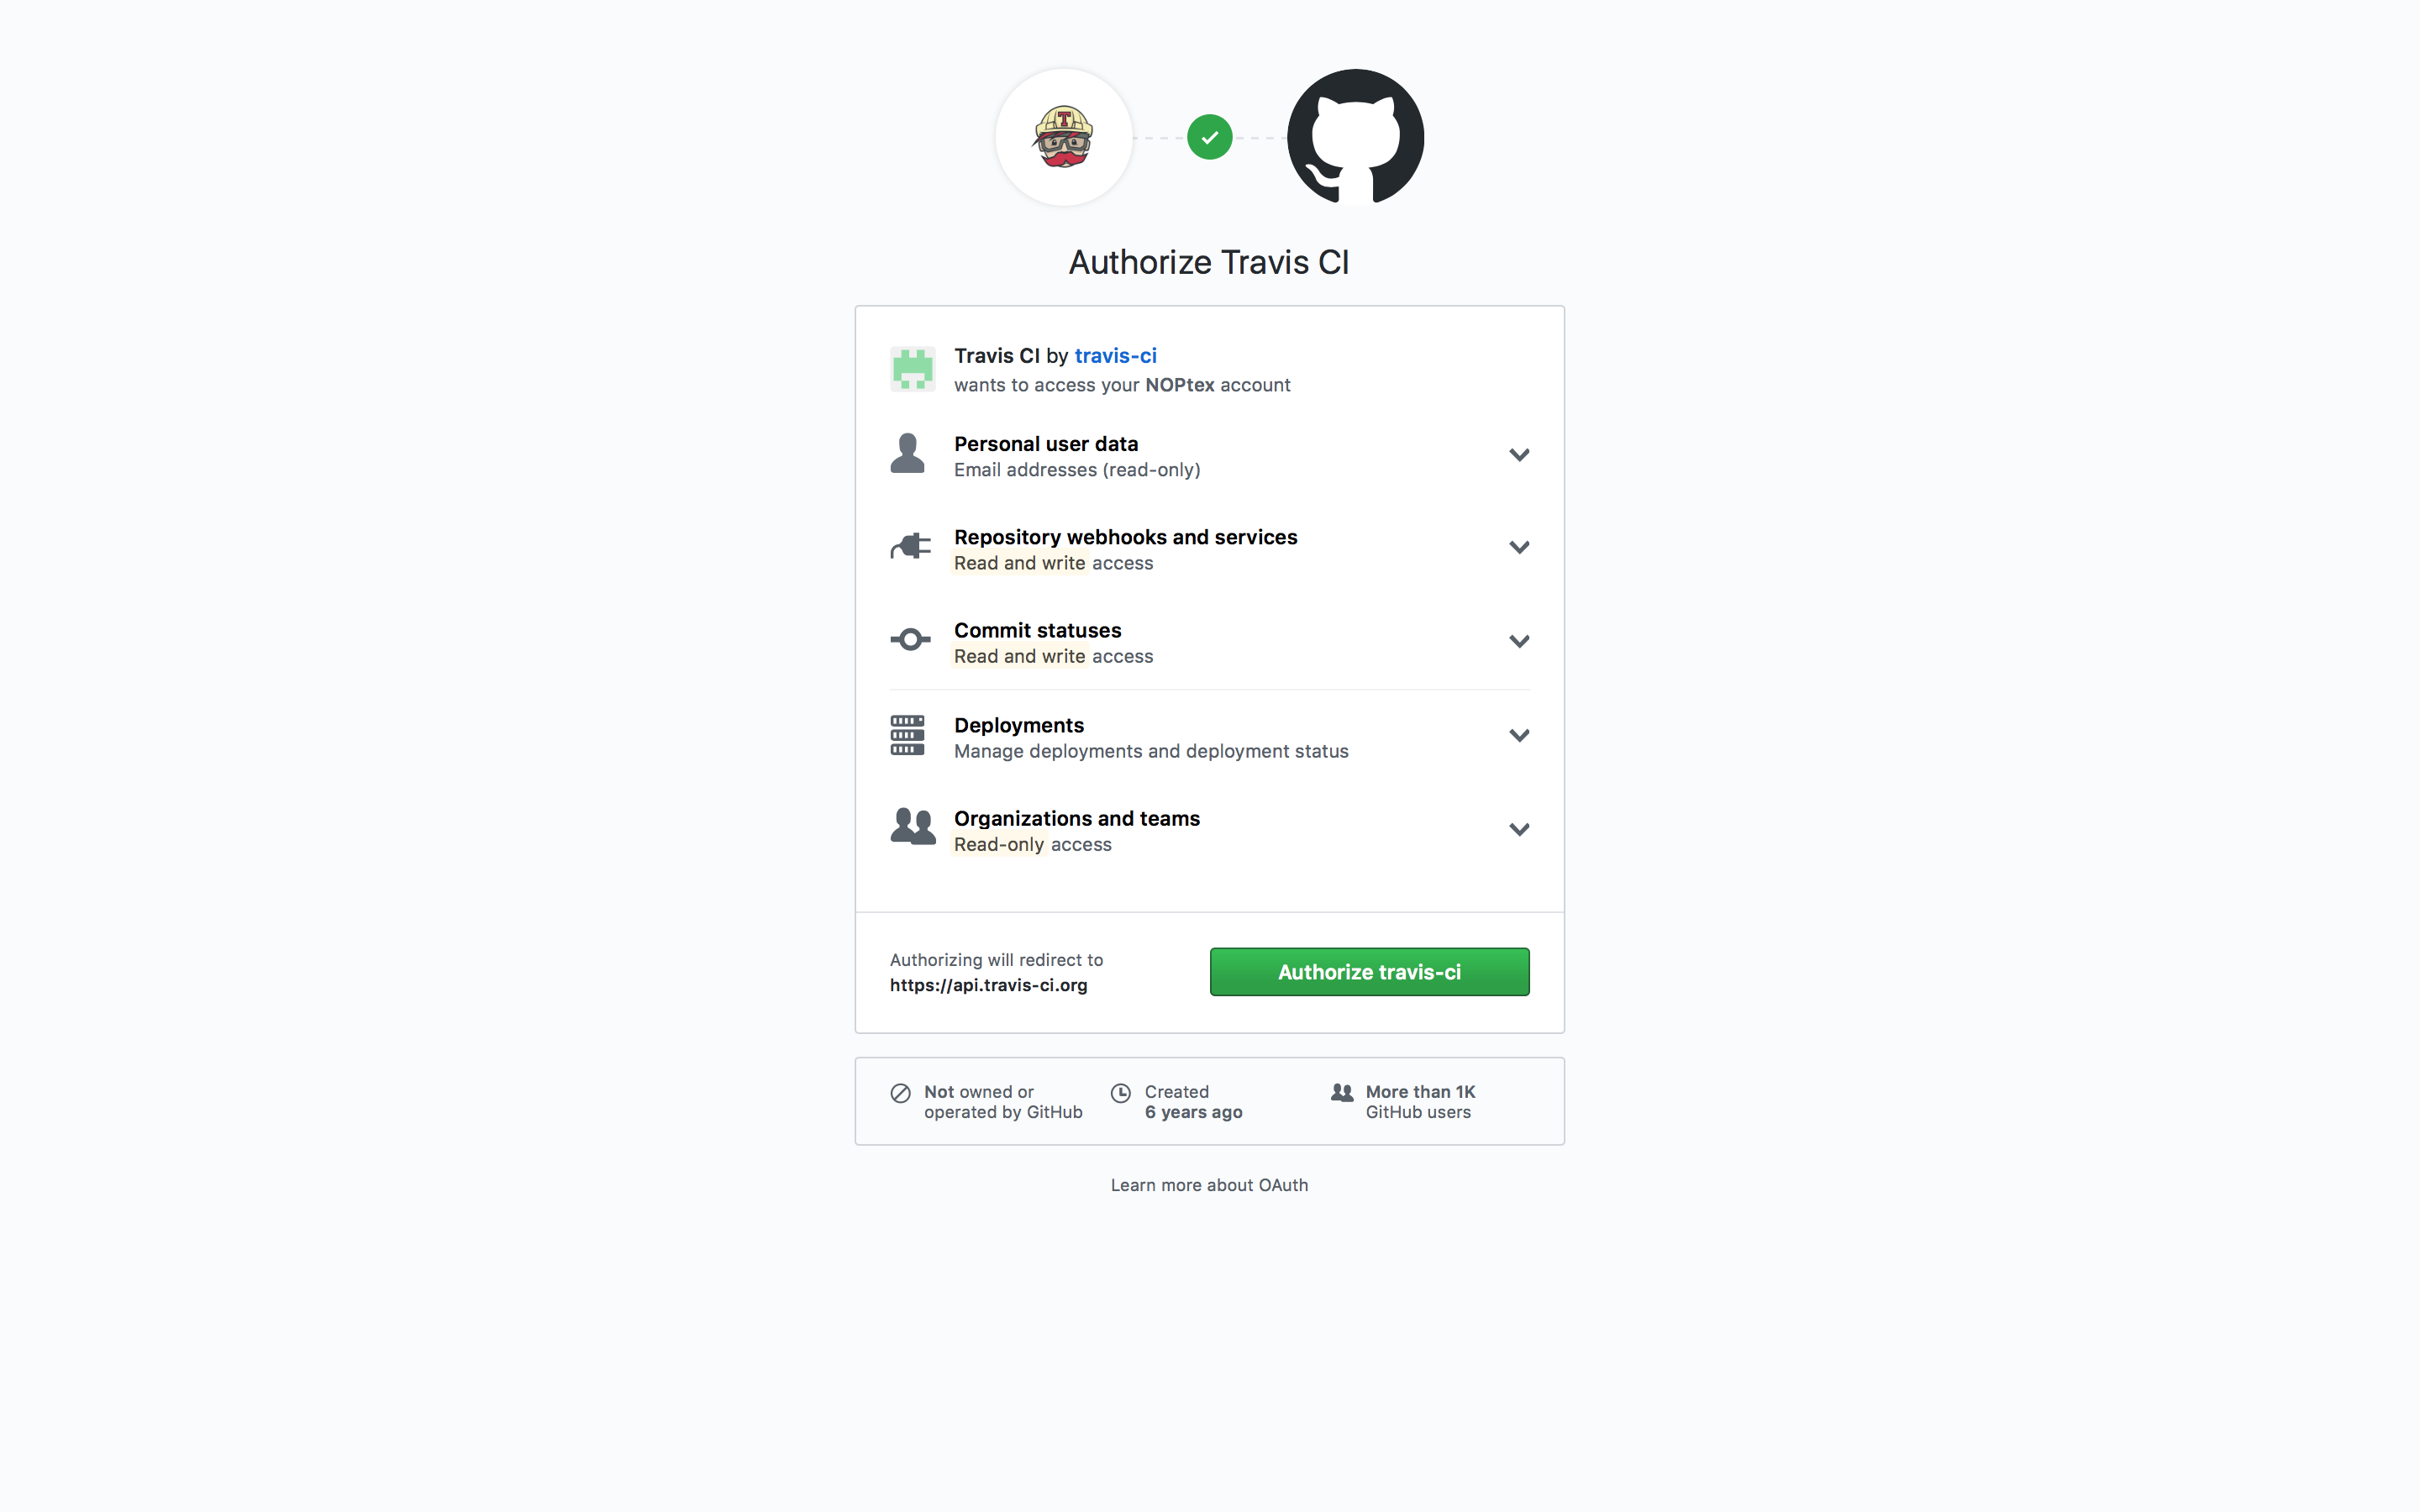
\includegraphics[width=1.0\textwidth]{./bilder/4TRAVISauthGITHUB.png}
\end{framed}

\end{minipage}}
\hfill
\adjustbox{valign=t}{\begin{minipage}[t]{0.45\textwidth}
\vspace{0pt}
\huge
Travis benötigt einige \\Berechtigungen welche man in diesem Schritt erteilt.
% \caption{Kapazität}
\end{minipage}}
\end{figure}

\clearpage % GleitObjekte anzeigen






\newpage % ============================================= Newpage ===================


\begin{figure}[ht]
  \subsubsection{Github - Repo aktivieren}
\adjustbox{valign=t}{\begin{minipage}[t]{0.50\textwidth}
\begin{framed}
  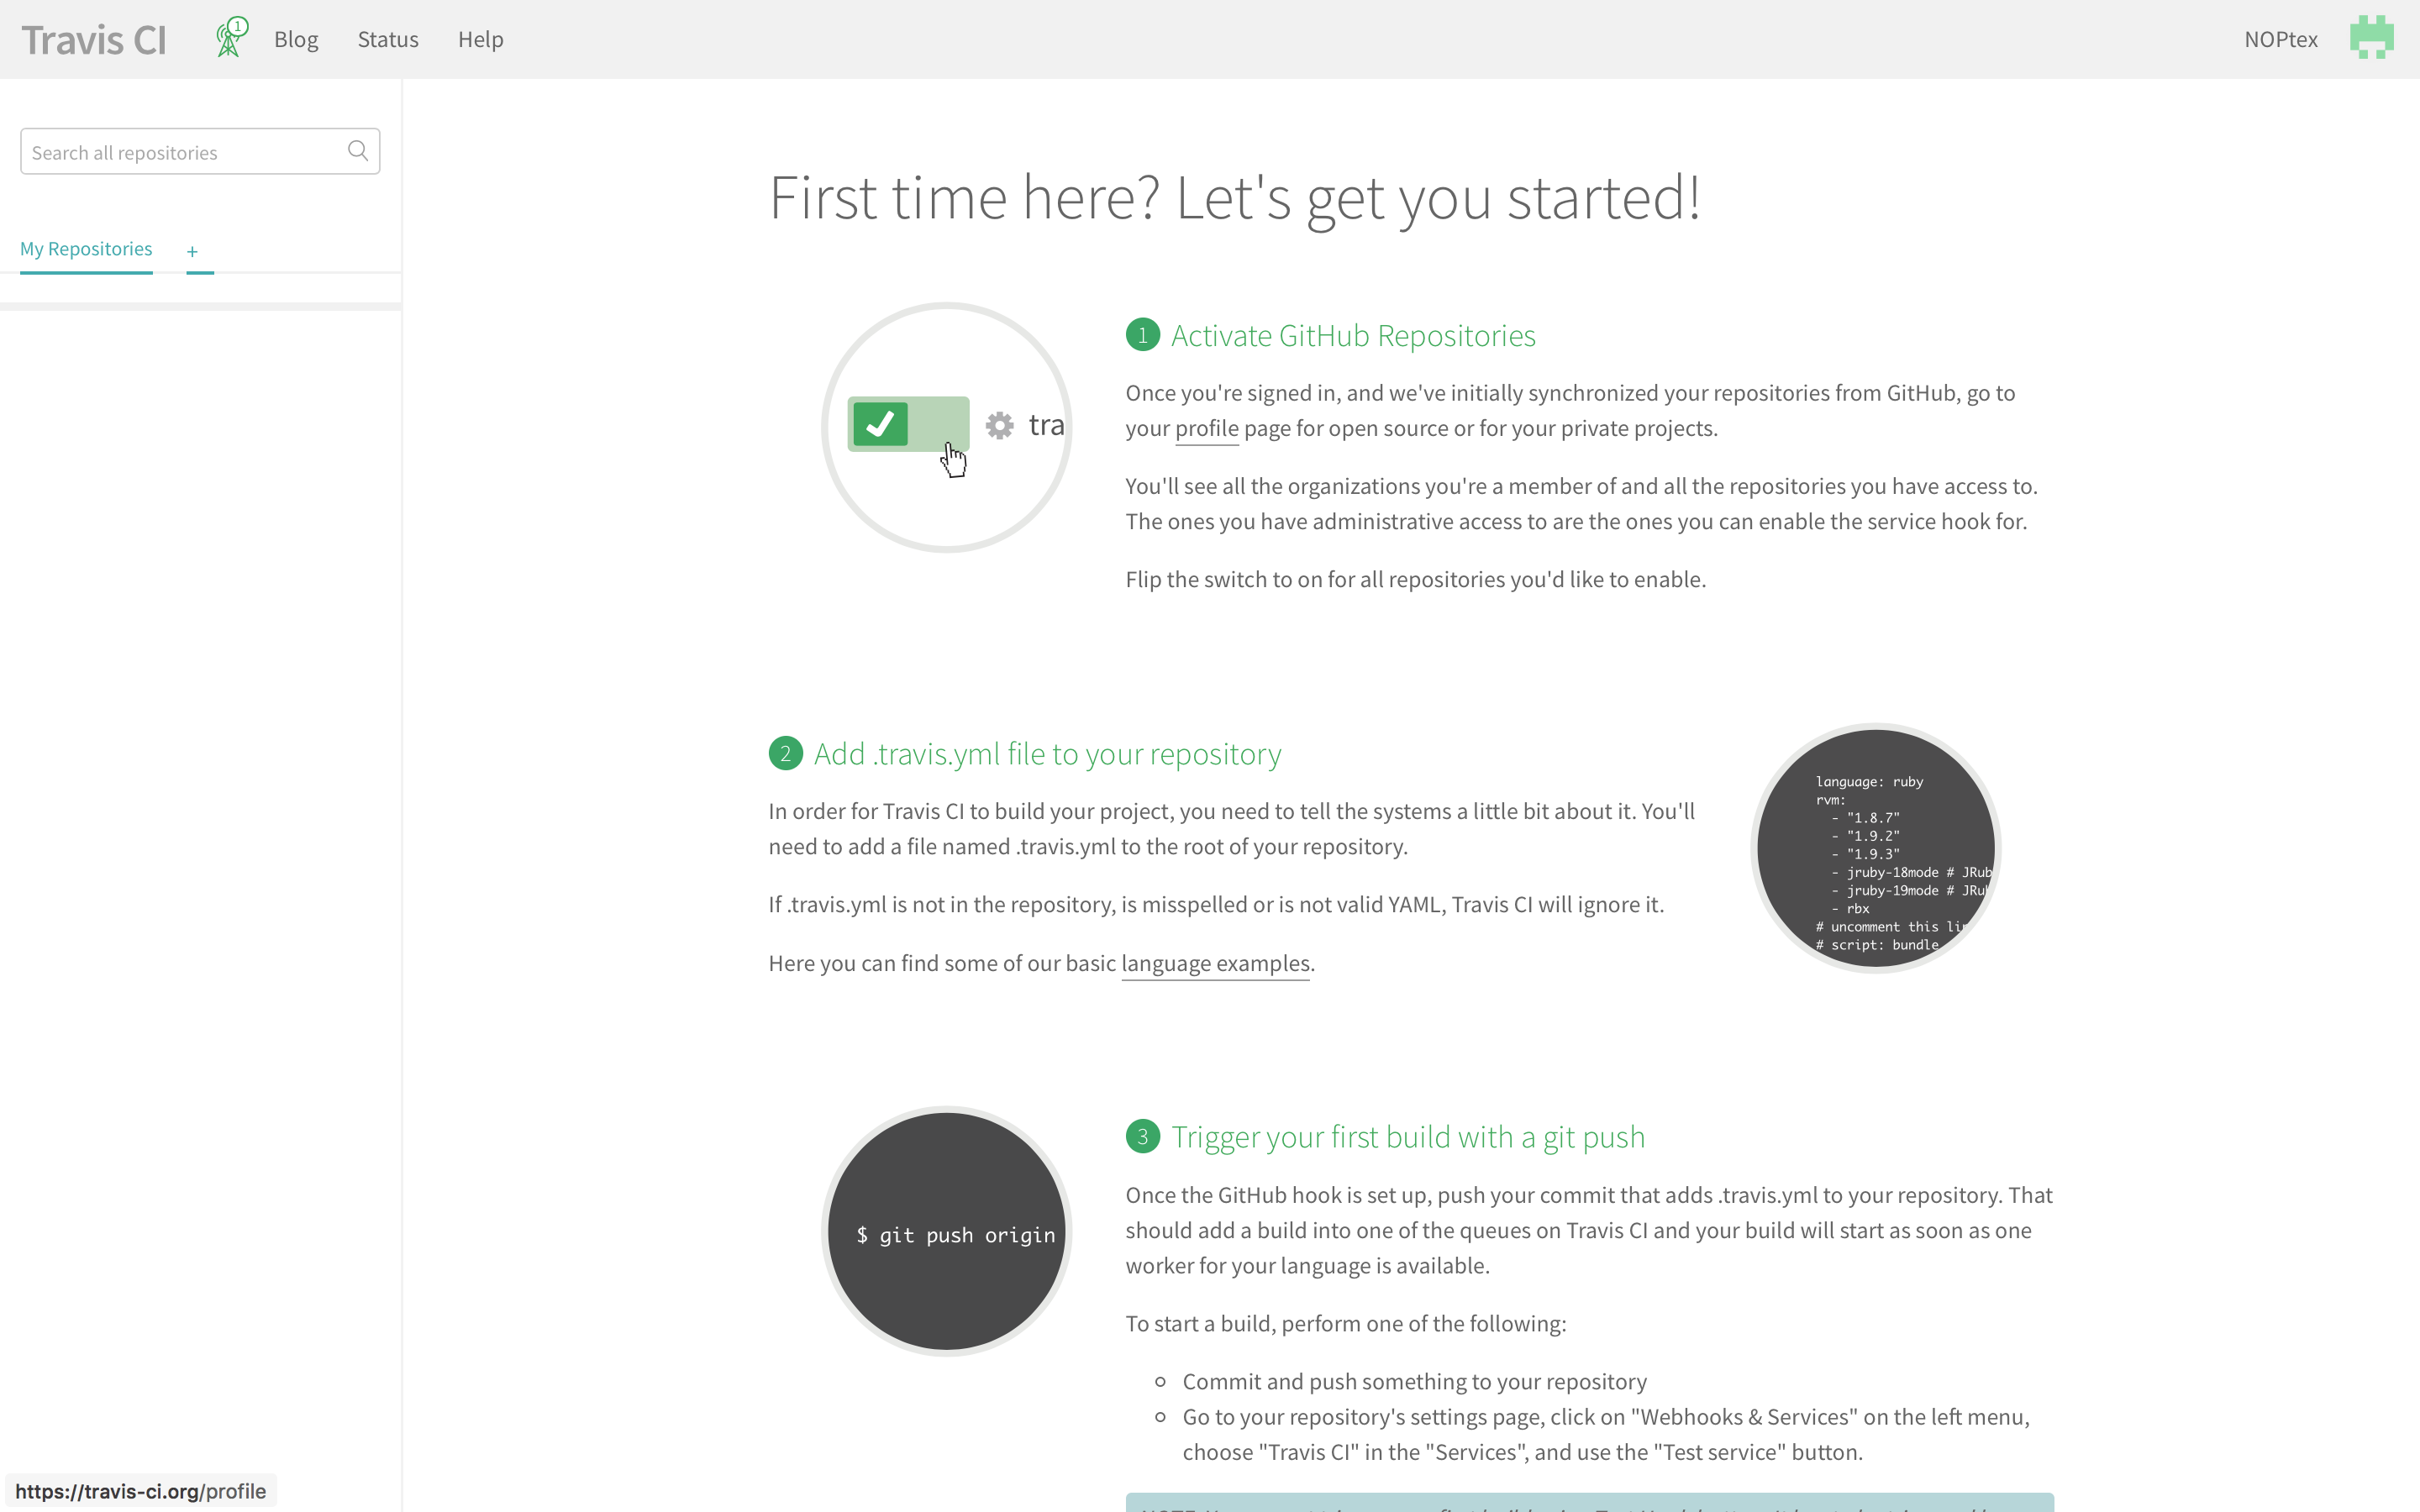
\includegraphics[width=1.0\textwidth]{./bilder/5TRAVISfirstSignIn.png}
\end{framed}

\end{minipage}}
% \hfill
\adjustbox{valign=t}{\begin{minipage}[t]{0.45\textwidth}
\vspace{0pt}
\huge
Da Travis nur mit Github funktioniert ist die Einrichtung recht einfach.
% \caption{Kapazität}
\end{minipage}}
% \end{figure}
% \vspace{0.5cm} % ----------------------------------- vspace
% \begin{figure}[ht]
\adjustbox{valign=t}{\begin{minipage}[t]{0.50\textwidth}
% \vspace{0.5cm}
\begin{framed}
  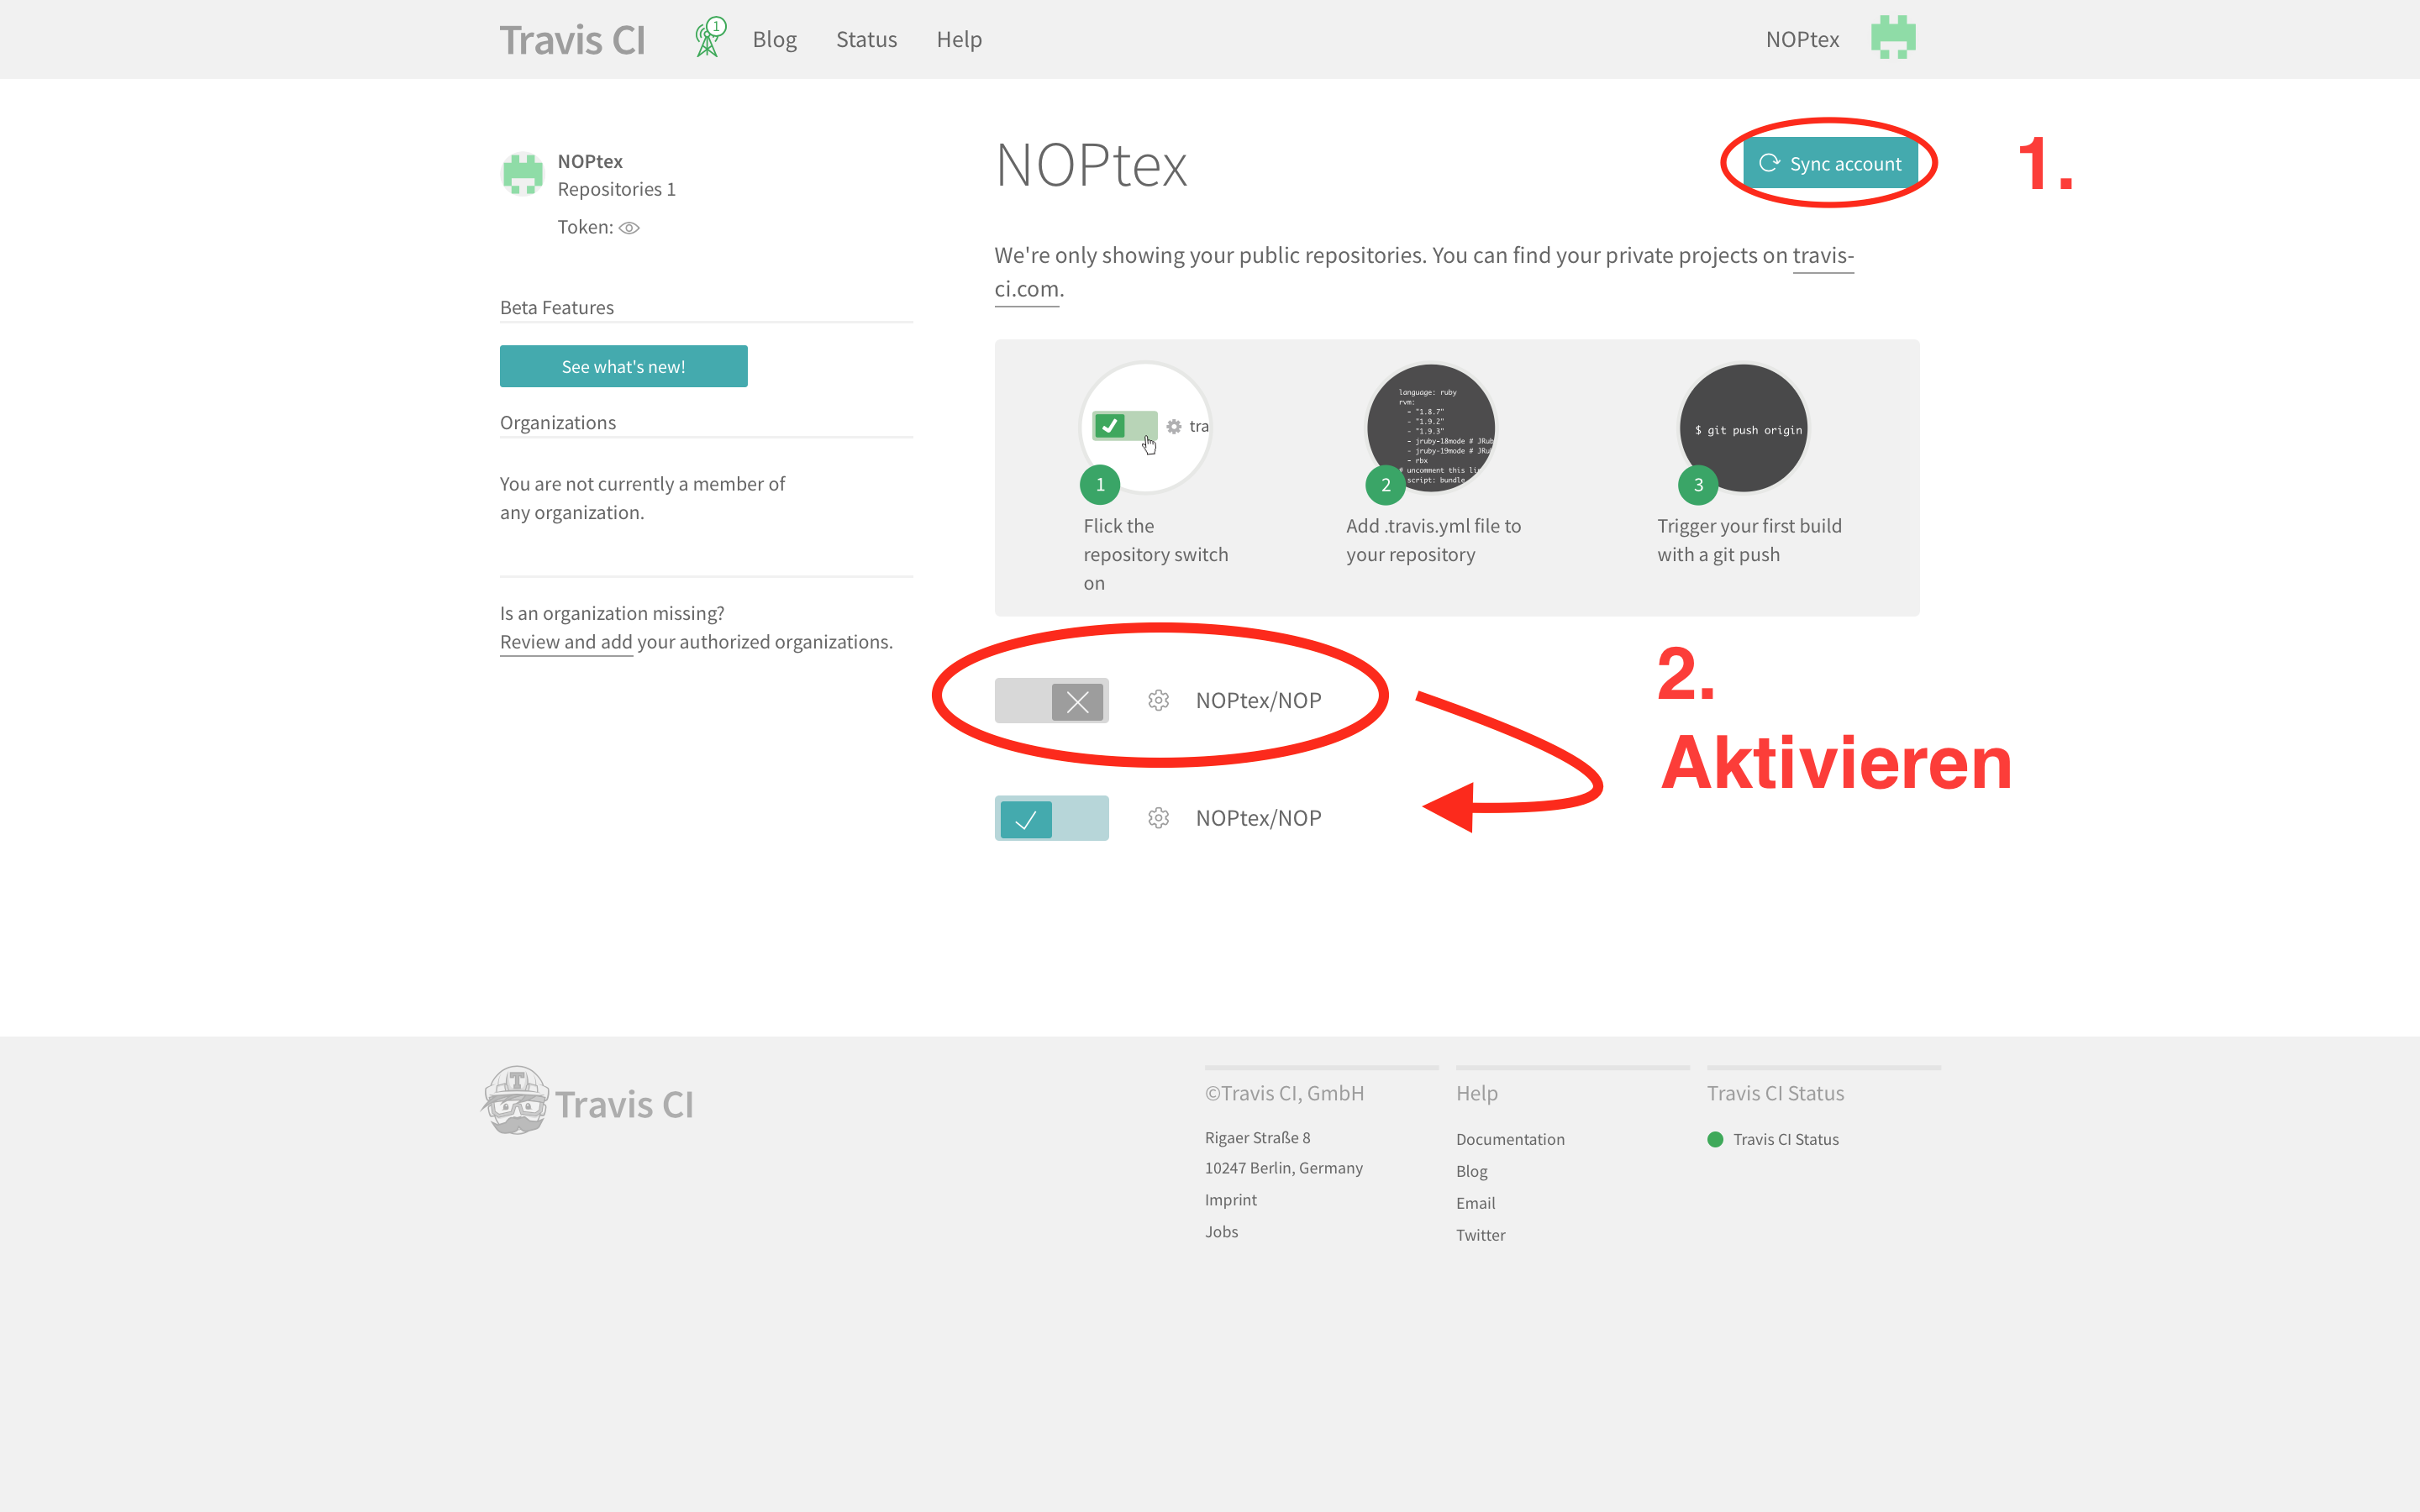
\includegraphics[width=1.0\textwidth]{./bilder/6TRAVISActivateREPO.png}
\end{framed}

\end{minipage}}
\hfill
\adjustbox{valign=t}{\begin{minipage}[t]{0.45\textwidth}
\vspace{0pt}
\huge
Travis benötigt einige Berechtigungen welche man im nächsten Schritt erteilt.
% \caption{Kapazität}
\end{minipage}}
\end{figure}

\clearpage % GleitObjekte anzeigen


\newpage % ============================================= Newpage ===================


\begin{figure}[ht]
  \subsubsection{Build-Einstellungen setzen}
\adjustbox{valign=t}{\begin{minipage}[t]{0.50\textwidth}
\begin{framed}
  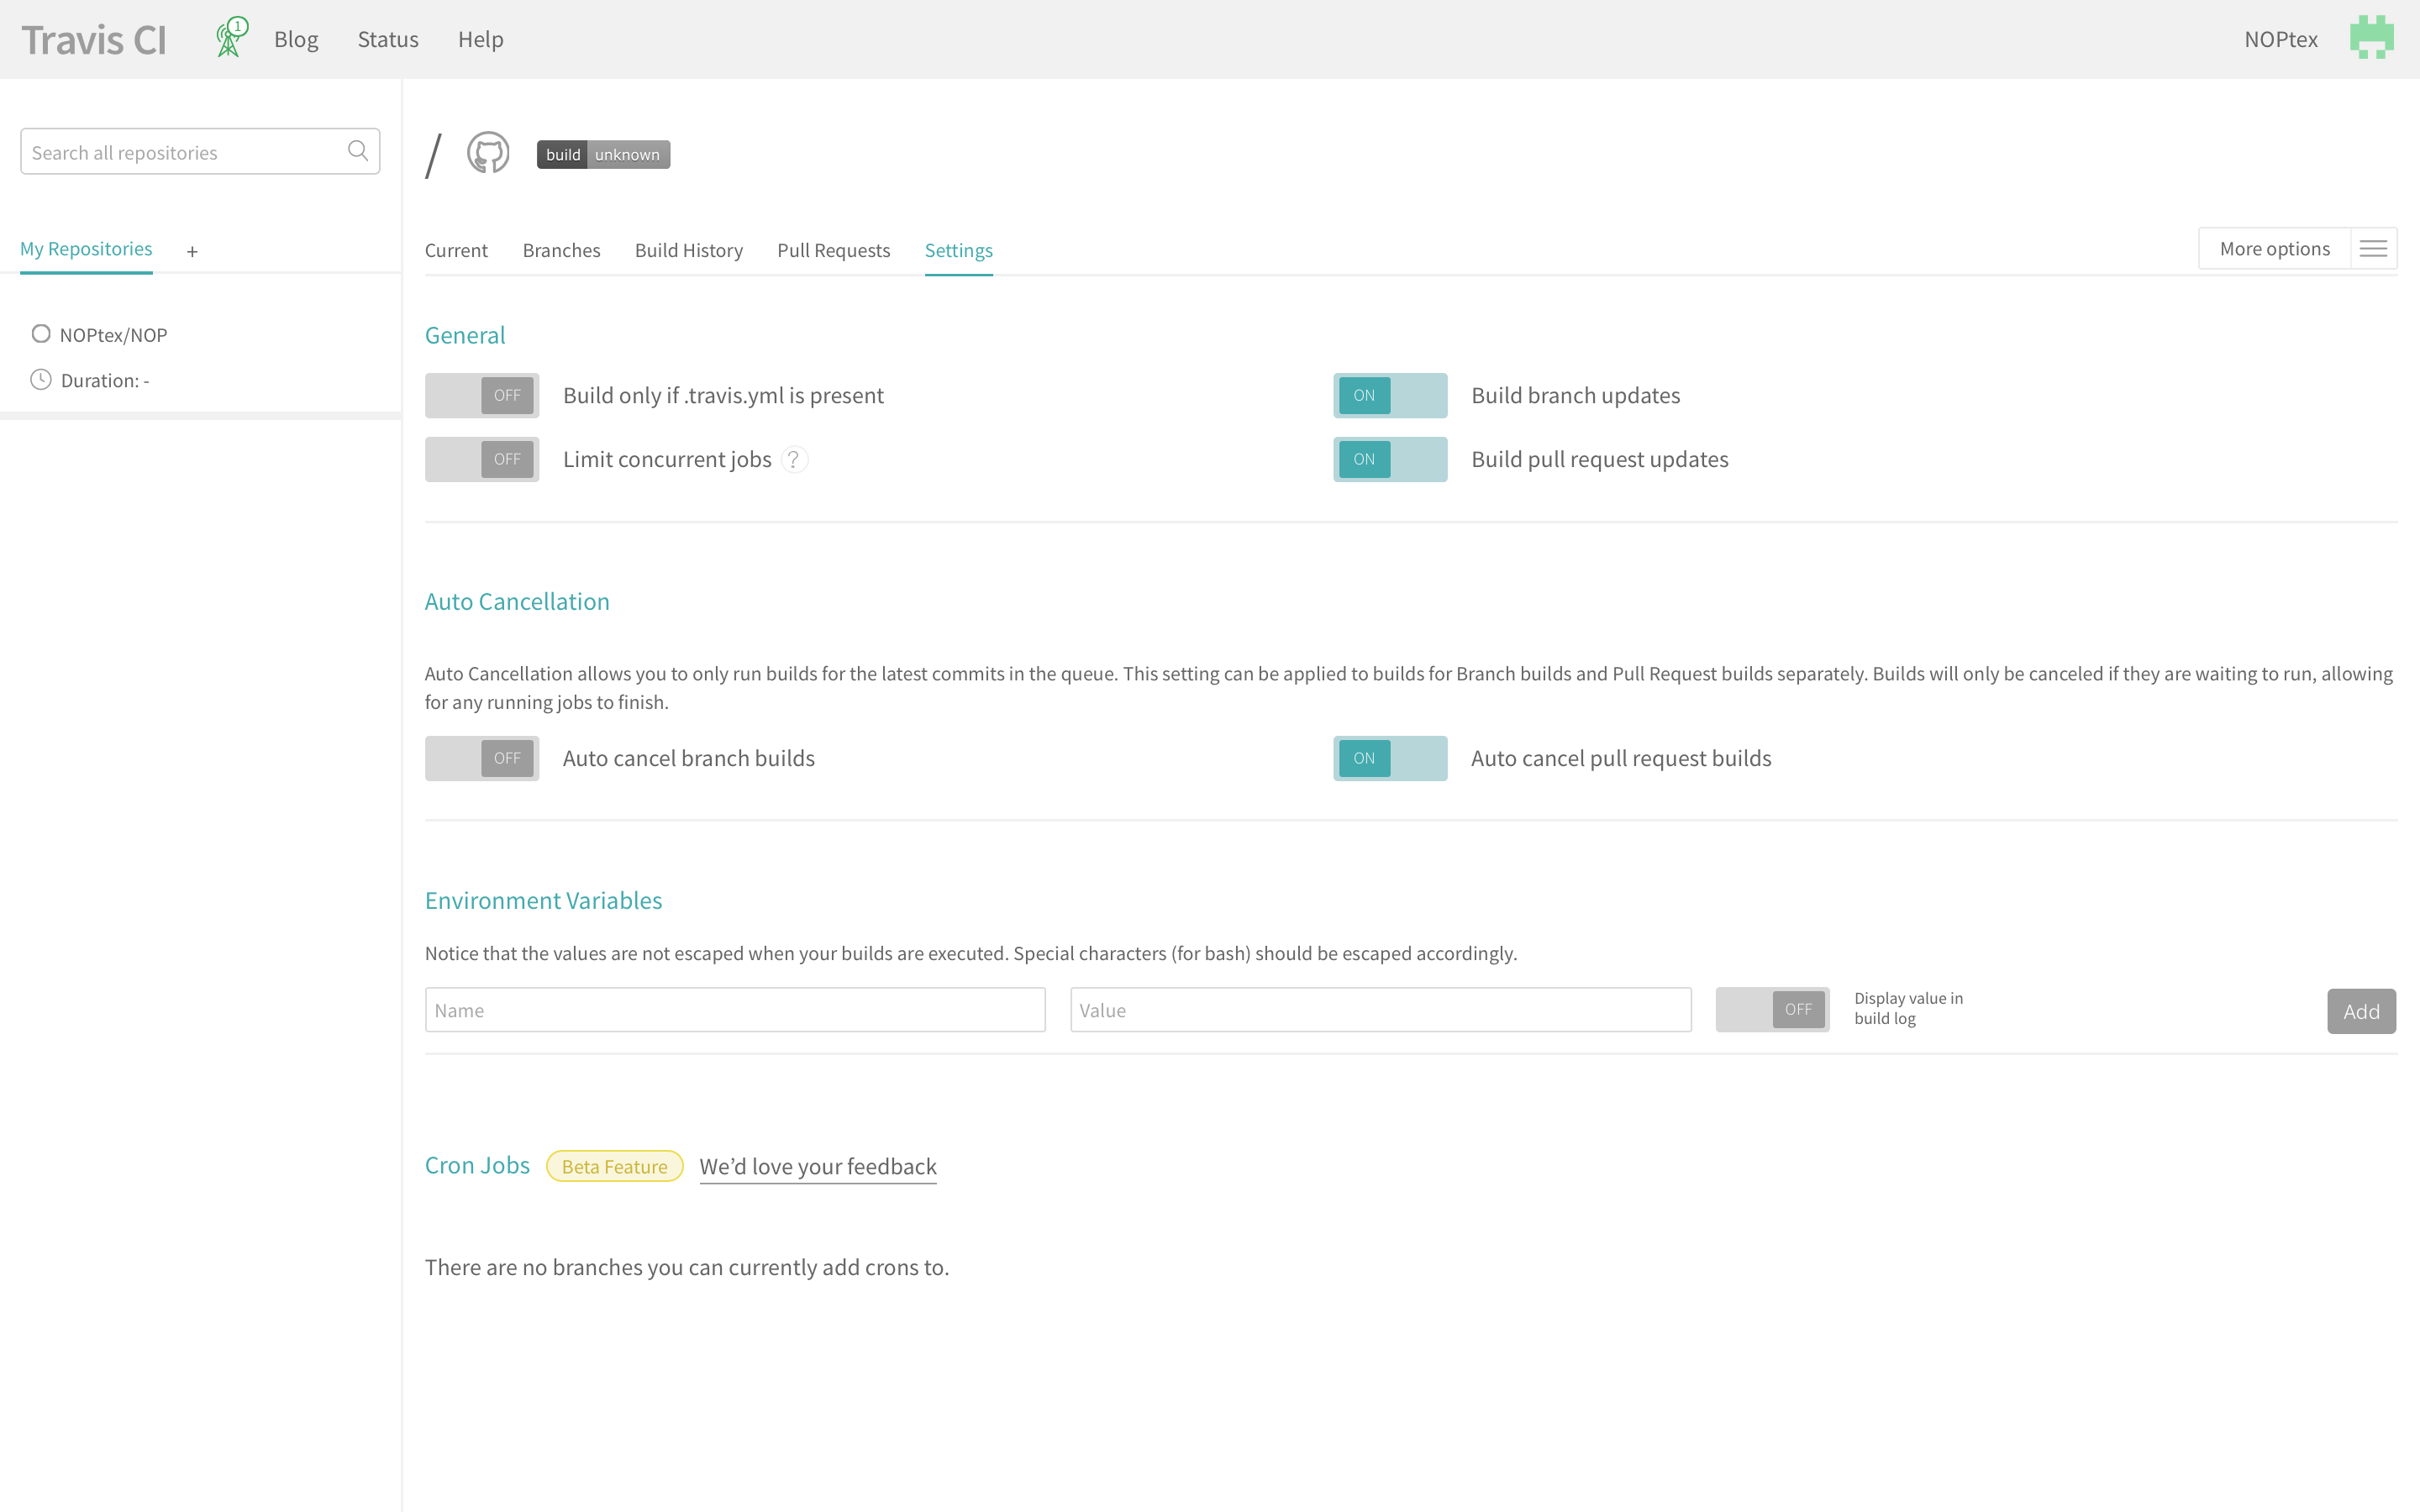
\includegraphics[width=1.0\textwidth]{./bilder/7TRAVISOptionsbase.png}
\end{framed}

\end{minipage}}
% \hfill
\adjustbox{valign=t}{\begin{minipage}[t]{0.45\textwidth}
\vspace{0pt}

\includegraphics[width=1.0\textwidth]{./bilder/7_1REPOsettings.png}
\huge
Über das Zahnrad kommt man zu den Einstellungen.
% \caption{Kapazität}
\end{minipage}}
% \end{figure}
% \vspace{0.5cm} % ----------------------------------- vspace
% \begin{figure}[ht]
\adjustbox{valign=t}{\begin{minipage}[t]{0.50\textwidth}
% \vspace{0.5cm}
\begin{framed}
  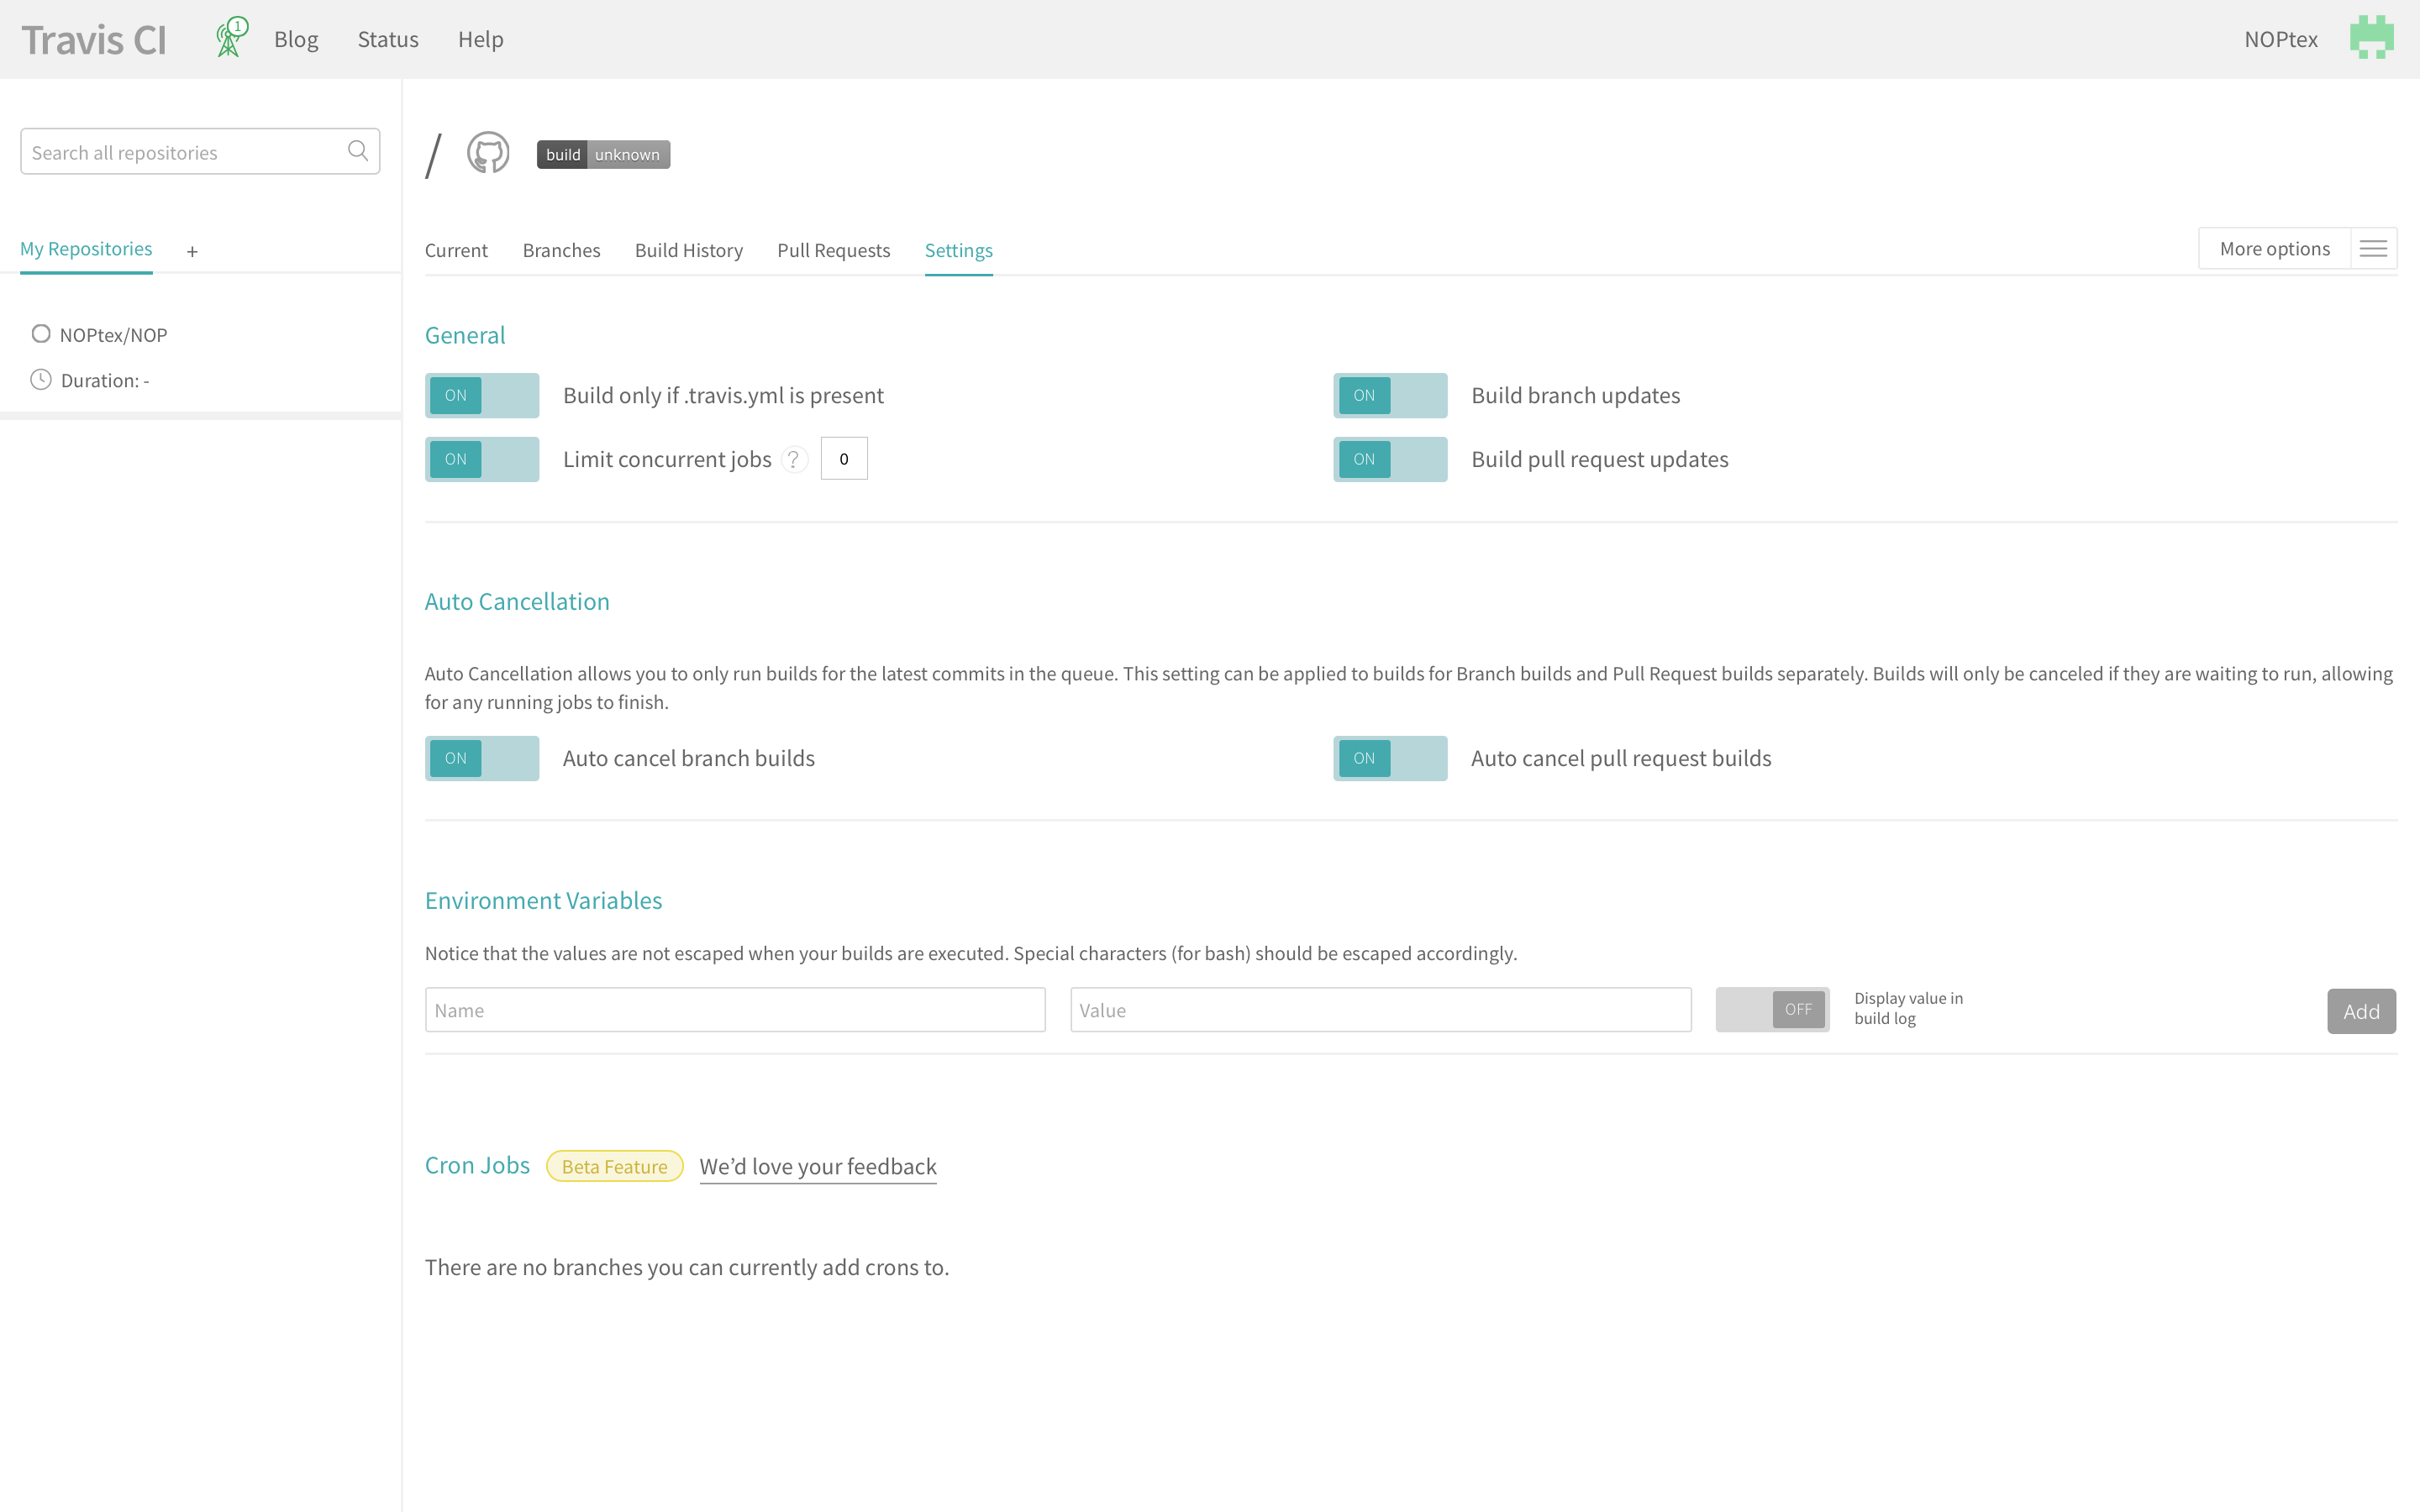
\includegraphics[width=1.0\textwidth]{./bilder/8TRAVISOptionsSET.png}
\end{framed}

\end{minipage}}
\hfill
\adjustbox{valign=t}{\begin{minipage}[t]{0.45\textwidth}
\vspace{0pt}
\huge
Ich setze alle Häkchen weil:
\begin{itemize}
  \item nur releases Gebaut werden sollen \\ (Testen kann man lokal) \\ Alle anderen Build sollen abgebrochen werden.
  \item Nur wenn .travis.yml vorhanden ist Build starten. \\(Einfaches deaktivieren über Git)
\end{itemize}
% \caption{Kapazität}
\end{minipage}}
\end{figure}

\clearpage % GleitObjekte anzeigen


%
% \newpage % ============================================= Newpage ===================
%
%
% \begin{figure}[ht]
%   \subsubsection{Build-Einstellungen setzen}
% \adjustbox{valign=t}{\begin{minipage}[t]{0.50\textwidth}
% \begin{framed}
%   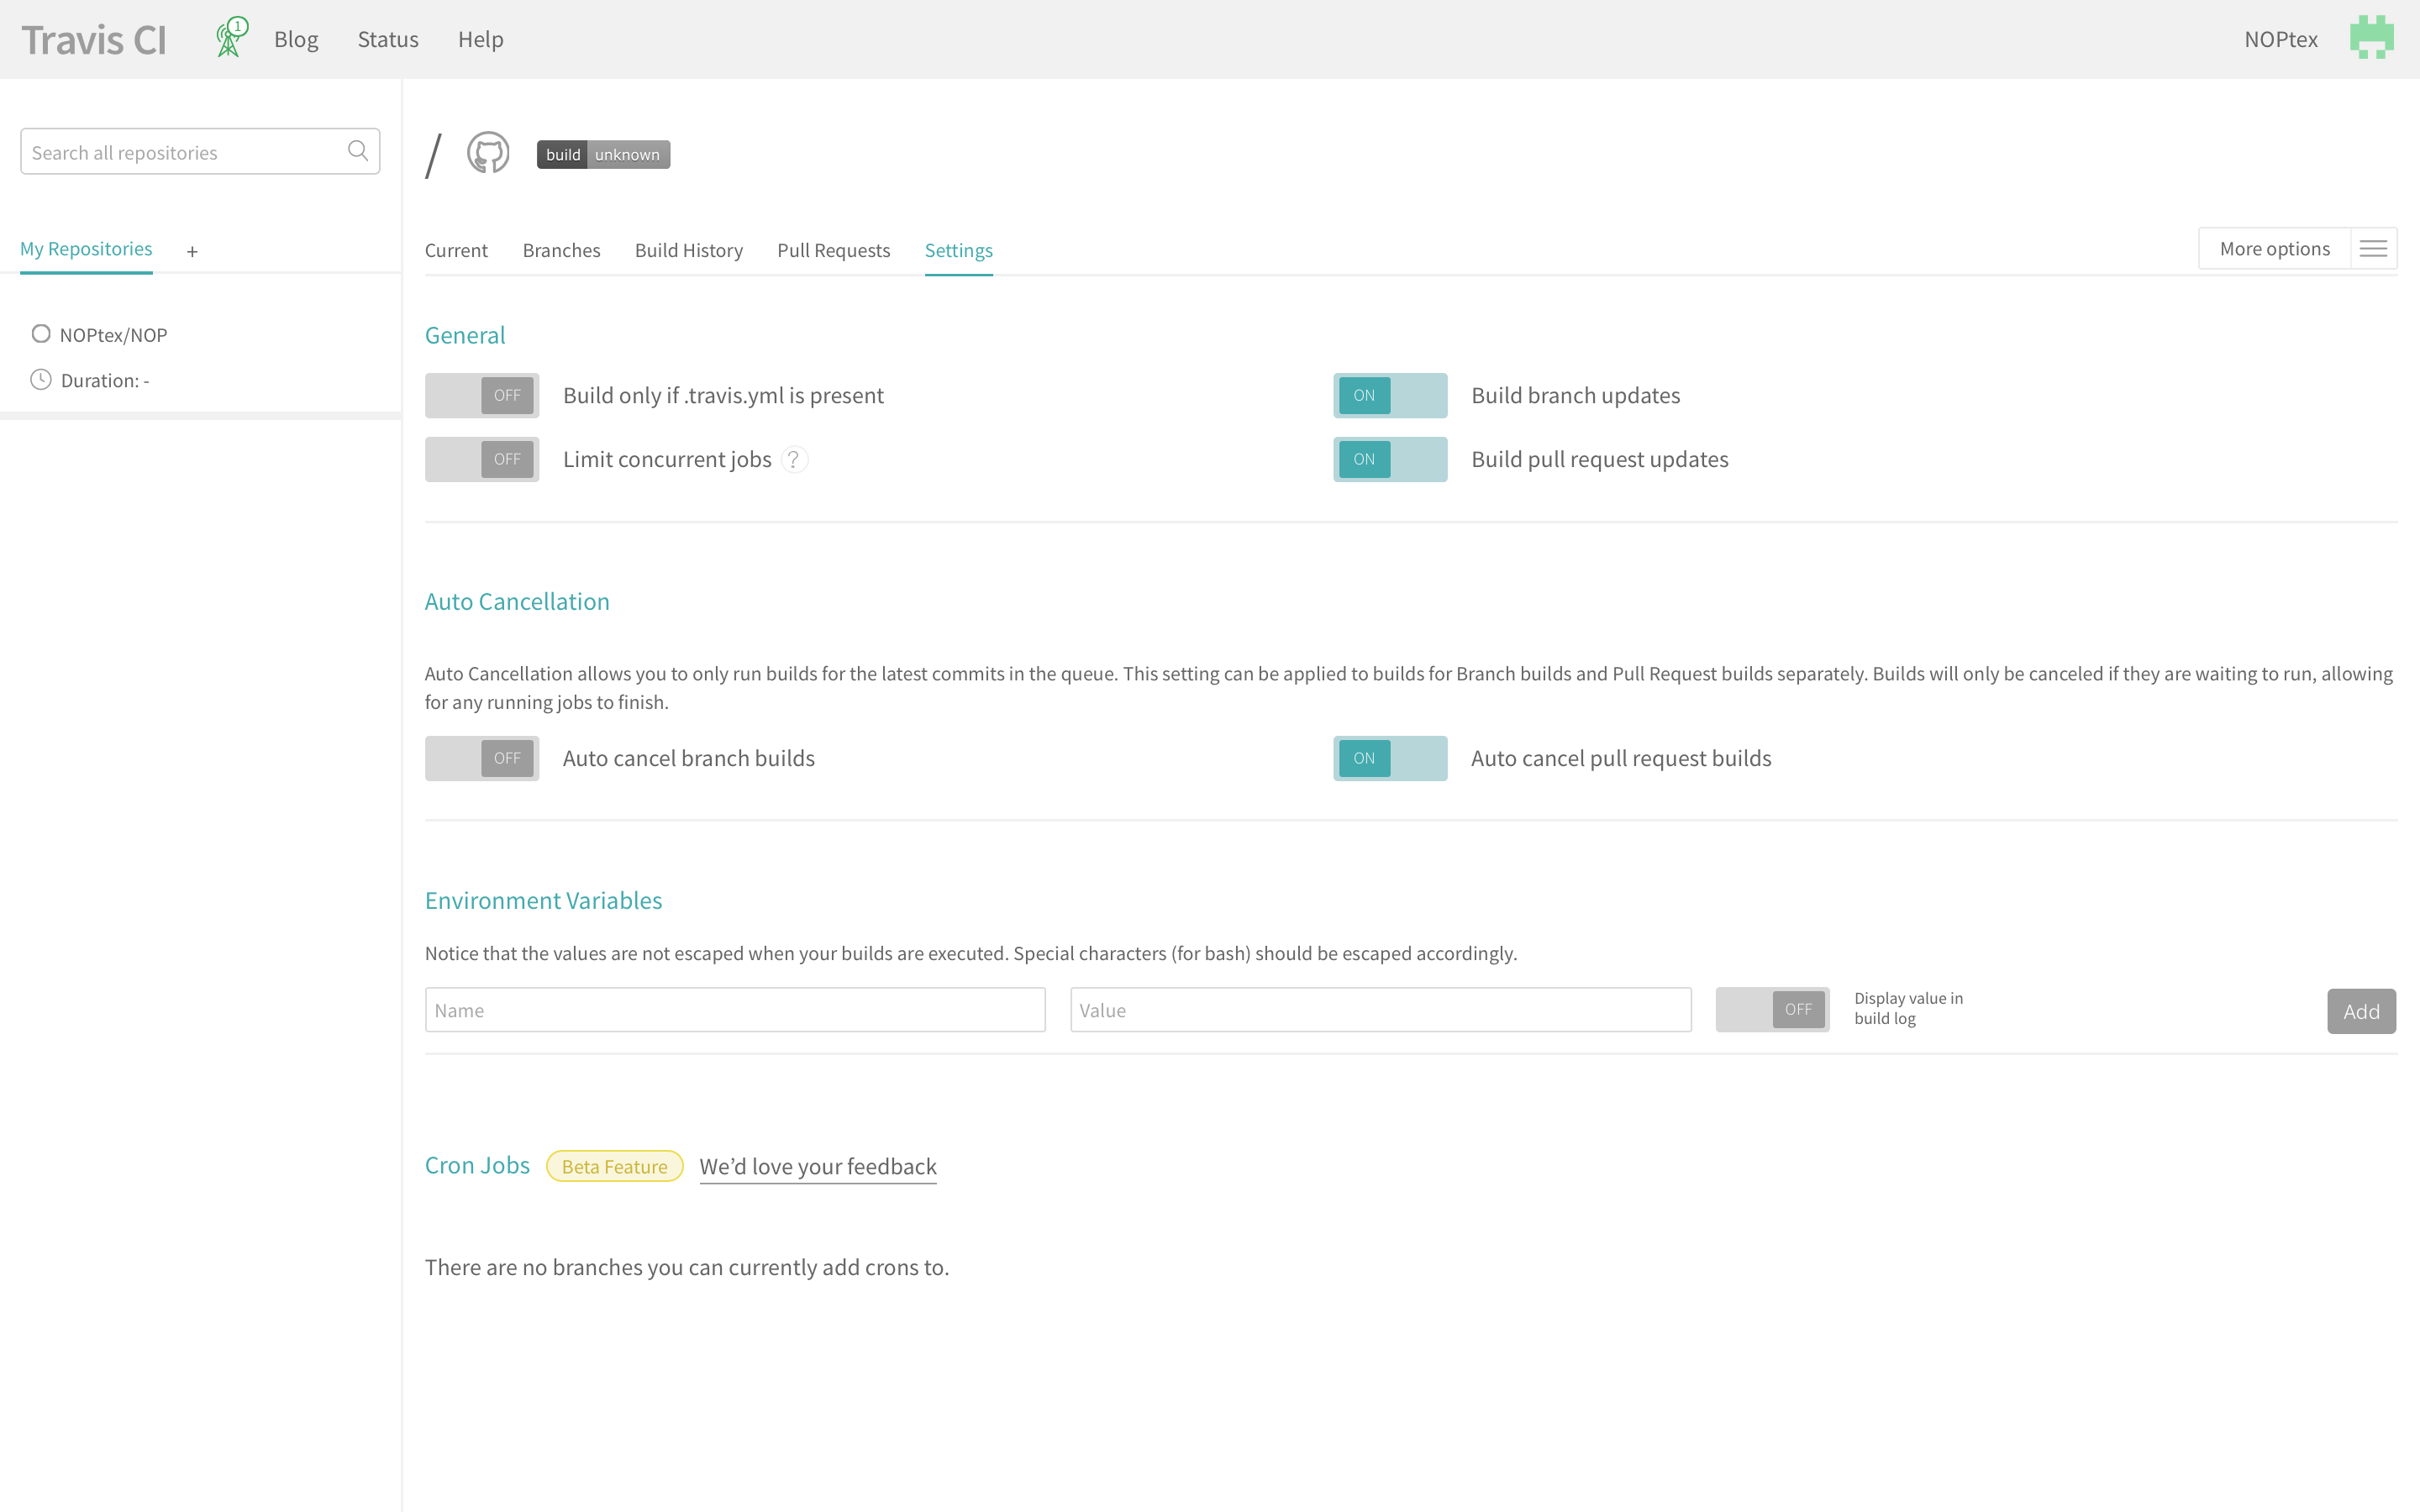
\includegraphics[width=1.0\textwidth]{./bilder/7TRAVISOptionsbase.png}
% \end{framed}
%
% \end{minipage}}
% % \hfill
% \adjustbox{valign=t}{\begin{minipage}[t]{0.45\textwidth}
% \vspace{0pt}
% 
\includegraphics[width=1.0\textwidth]{./bilder/7_1REPOsettings.png}
% \huge
% Über das Zahnrad kommt man zu den Einstellungen.
% % \caption{Kapazität}
% \end{minipage}}
% % \end{figure}
% % \vspace{0.5cm} % ----------------------------------- vspace
% % \begin{figure}[ht]
% \adjustbox{valign=t}{\begin{minipage}[t]{0.50\textwidth}
% % \vspace{0.5cm}
% \begin{framed}
%   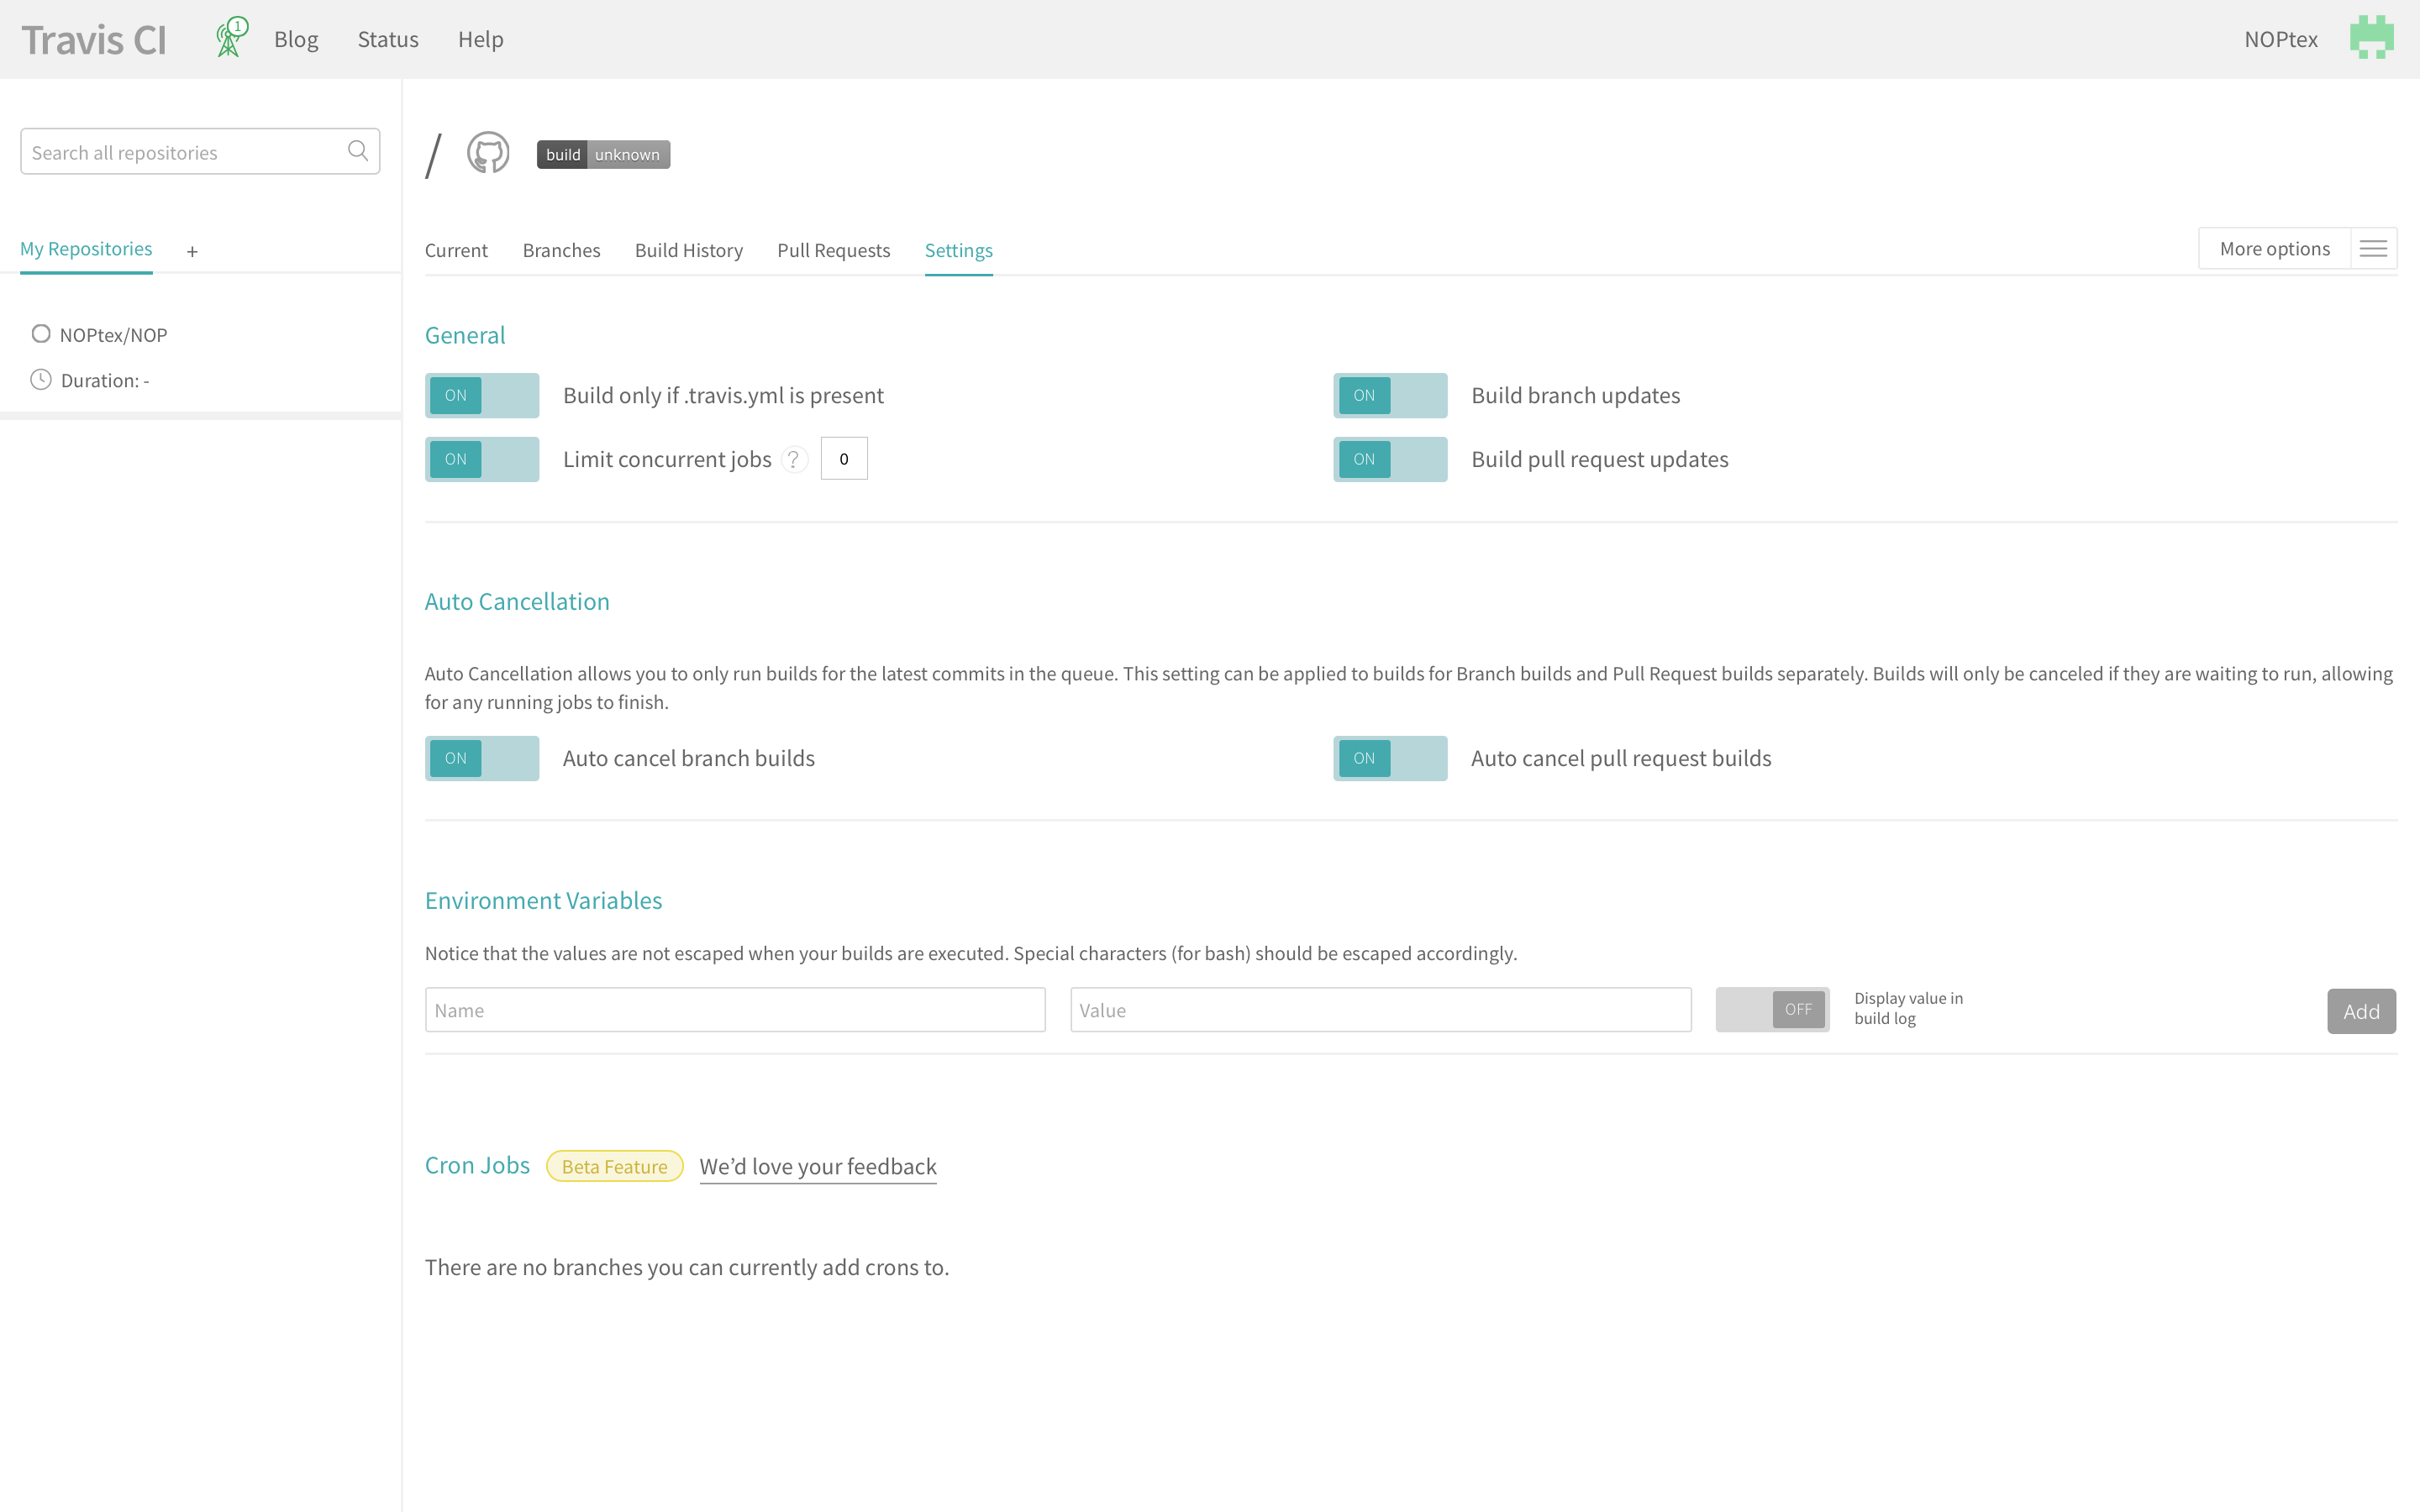
\includegraphics[width=1.0\textwidth]{./bilder/8TRAVISOptionsSET.png}
% \end{framed}
%
% \end{minipage}}
% \hfill
% \adjustbox{valign=t}{\begin{minipage}[t]{0.45\textwidth}
% \vspace{0pt}
% \huge
% Ich setze alle Häkchen weil:
% \begin{itemize}
%   \item nur releases Gebaut werden sollen \\ (Testen kann man lokal) \\ Alle anderen Build sollen abgebrochen werden.
%   \item Nur wenn .travis.yml vorhanden ist Build starten. \\(Einfaches deaktivieren über Git)
% \end{itemize}
% % \caption{Kapazität}
% \end{minipage}}
% \end{figure}
%
% \clearpage % GleitObjekte anzeigen
    % Latex the PDF LAtex way
\newpage
\section{Das wars? $\rightsquigarrow$  Nicht ganz !}
\subsection{Travis YAML erstellen/anpassen}
Da die Kommunikation zwischen Travis und GitHub verschlüsselt abläuft, muss man sich einen eigenen Schlüssel erstellen.

Am einfachsten geht das mit dem Travis-Komandozeilenprogramm.\\
Doch zuerst sollte man sich die vorhandene .travis.yml sichern.
\vspace{0.3cm}
\monocodebox{sh}{.travis.yml sichern}{./code/travis.sh}{false}{4}{9}
\subsection{eine neue .travis.yml erstellen}
\monocodebox{sh}{Basis-Datei erstellen}{./code/travis.sh}{false}{11}{22}

\newpage
Danach wurde eine Datei mit folgendem Inhalt generiert:
\monocodebox{sh}{Basis-Datei erstellen}{./code/travis.sh}{false}{27}{33}

\newpage
Jetzt muss man denn Rest wieder einfügen:

\monocodebox{sh}{Hinzufuegen der noetigen Aenderungen}{./code/travis.sh}{true}{41}{51}

\newpage
Fortsetzung:

\monocodebox{sh}{Hinzufuegen der nötigen Änderungen}{./code/travis.sh}{true}{58}{67}

\newpage
Deploy:

\monocodebox{sh}{Hinzufuegen der nötigen Änderungen}{./code/travis.sh}{true}{71}{76}


\newpage % ============================================= Newpage ===================


\begin{figure}[ht]
  \section{Release mit Tag erstellen und bauen}
\adjustbox{valign=t}{\begin{minipage}[t]{0.50\textwidth}
\begin{framed}
  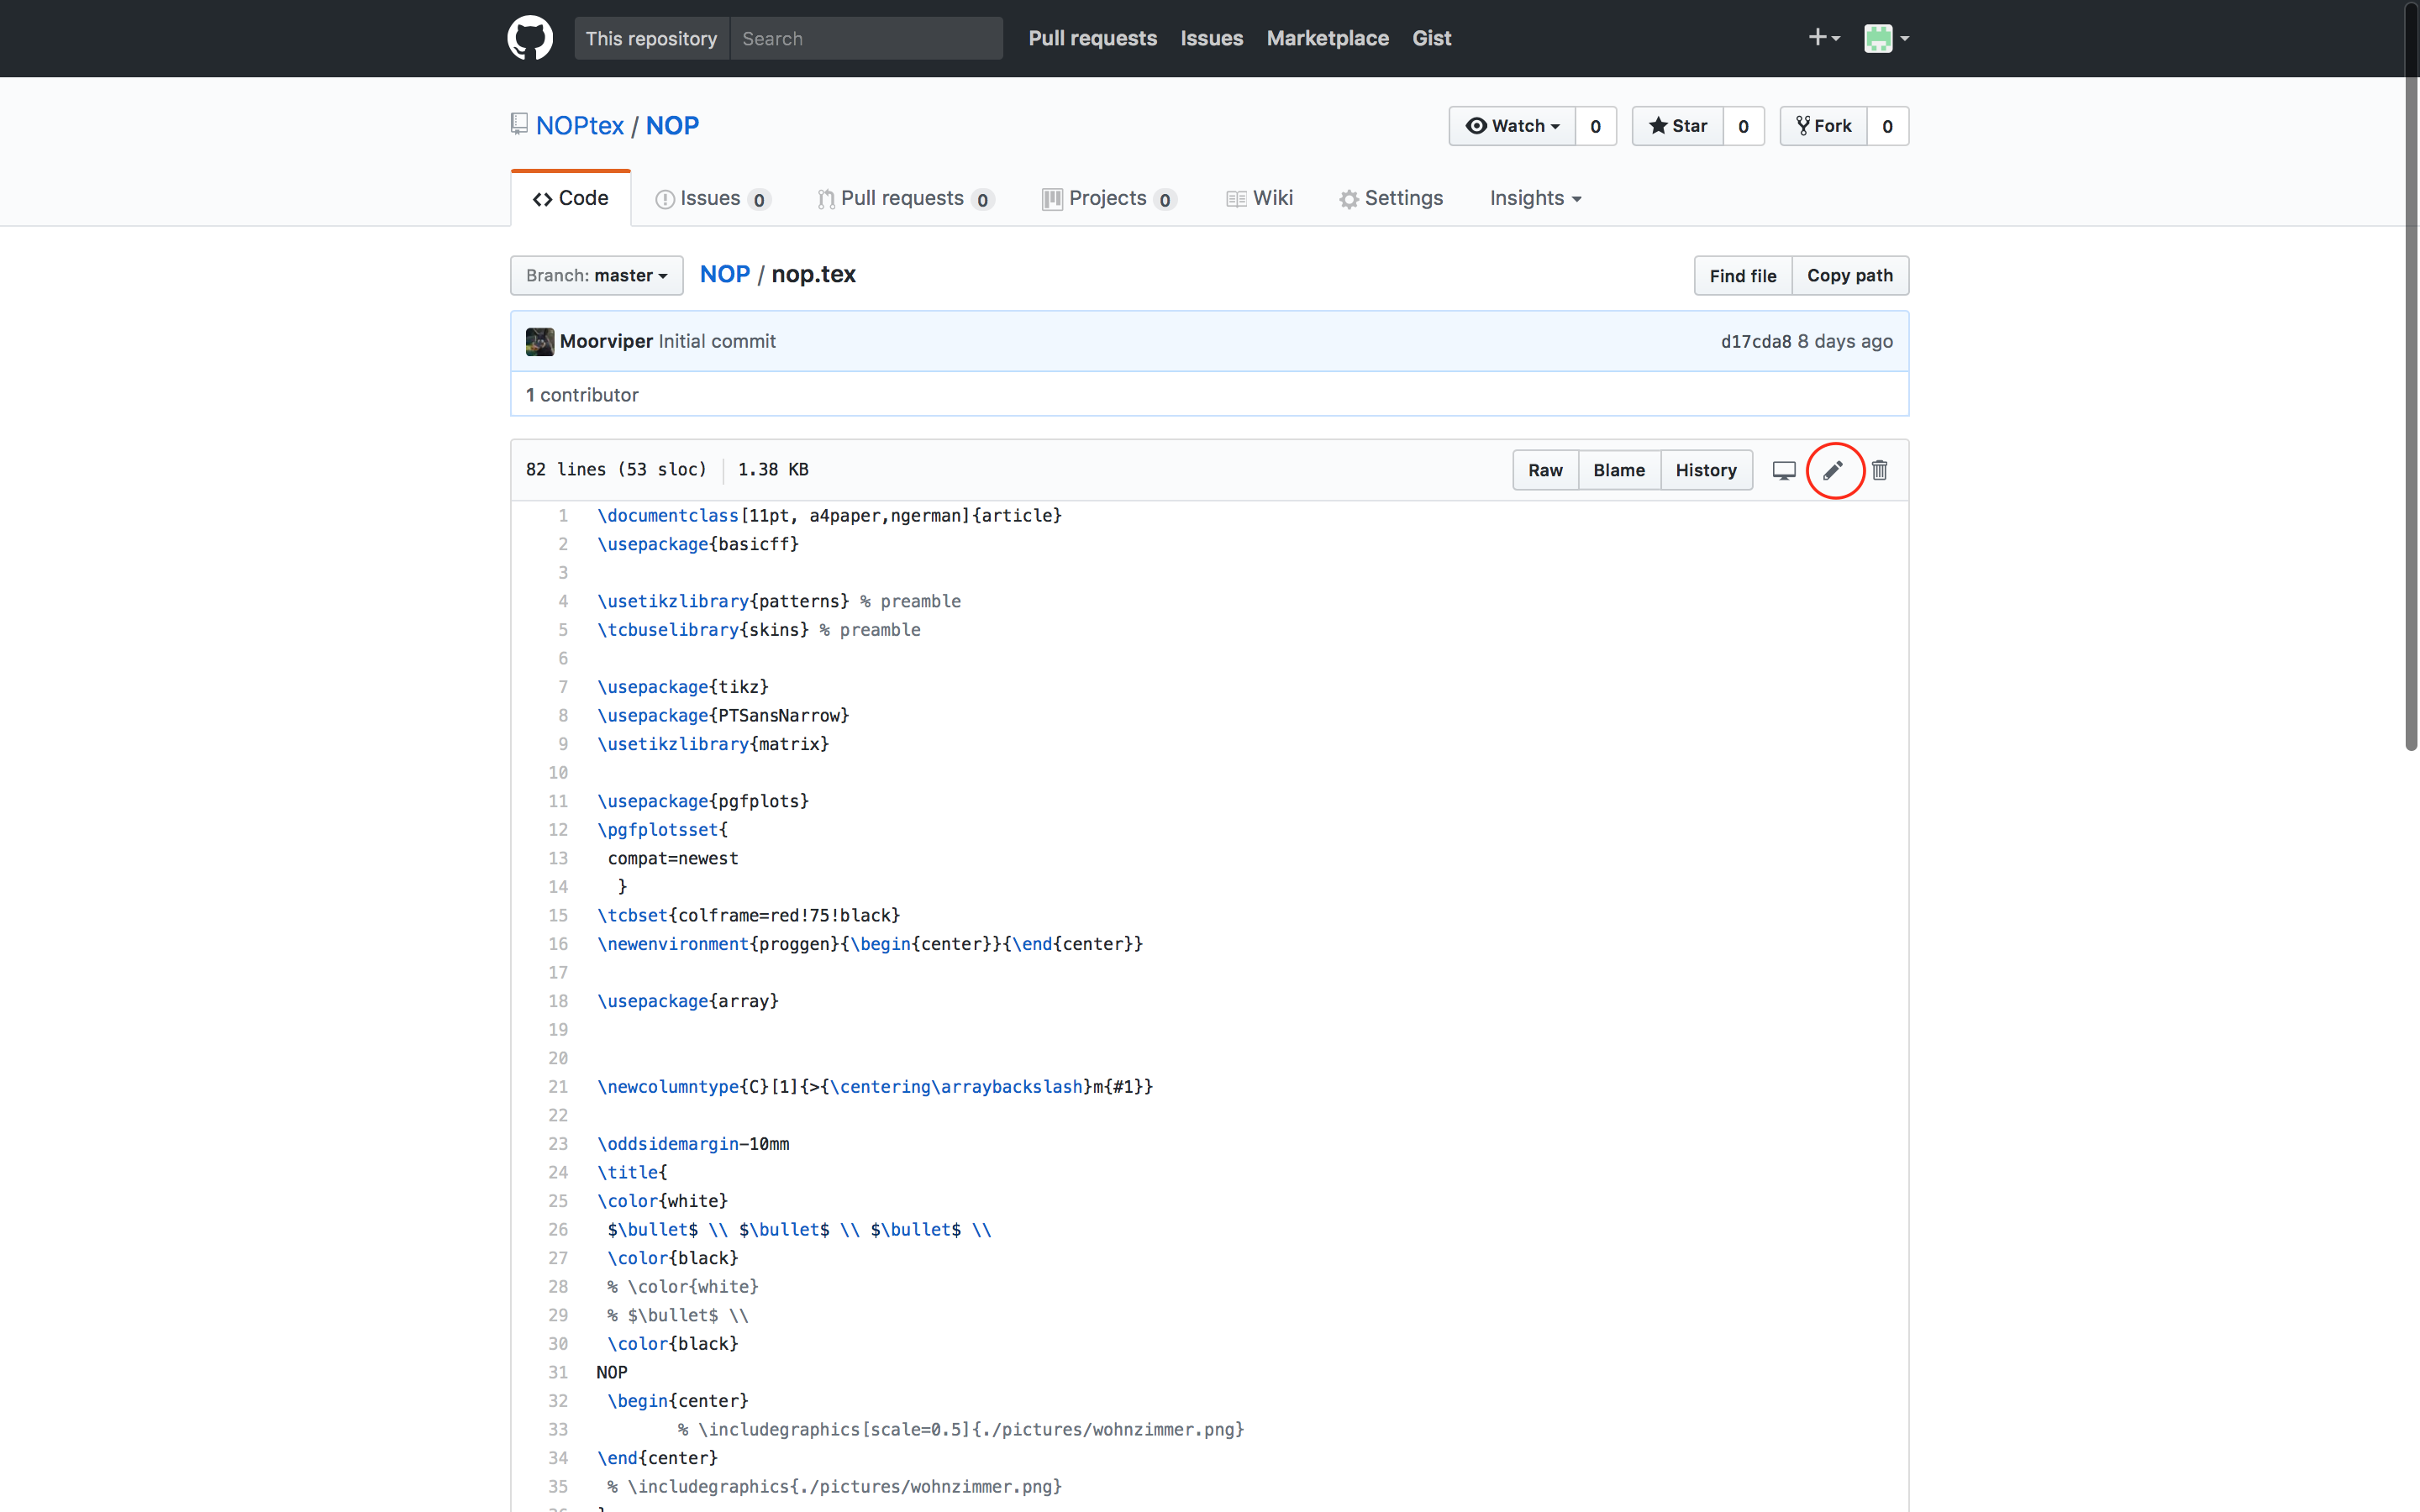
\includegraphics[width=1.0\textwidth]{./bilder/21edit.png}
\end{framed}

\end{minipage}}
% \hfill
\adjustbox{valign=t}{\begin{minipage}[t]{0.45\textwidth}
\vspace{0pt}
\huge
Man klickt auf den Stift zum editieren der Datei.
% \caption{Kapazität}
\end{minipage}}
% \end{figure}
% \vspace{0.5cm} % ----------------------------------- vspace
% \begin{figure}[ht]
\adjustbox{valign=t}{\begin{minipage}[t]{0.50\textwidth}
% \vspace{0.5cm}
\begin{framed}
  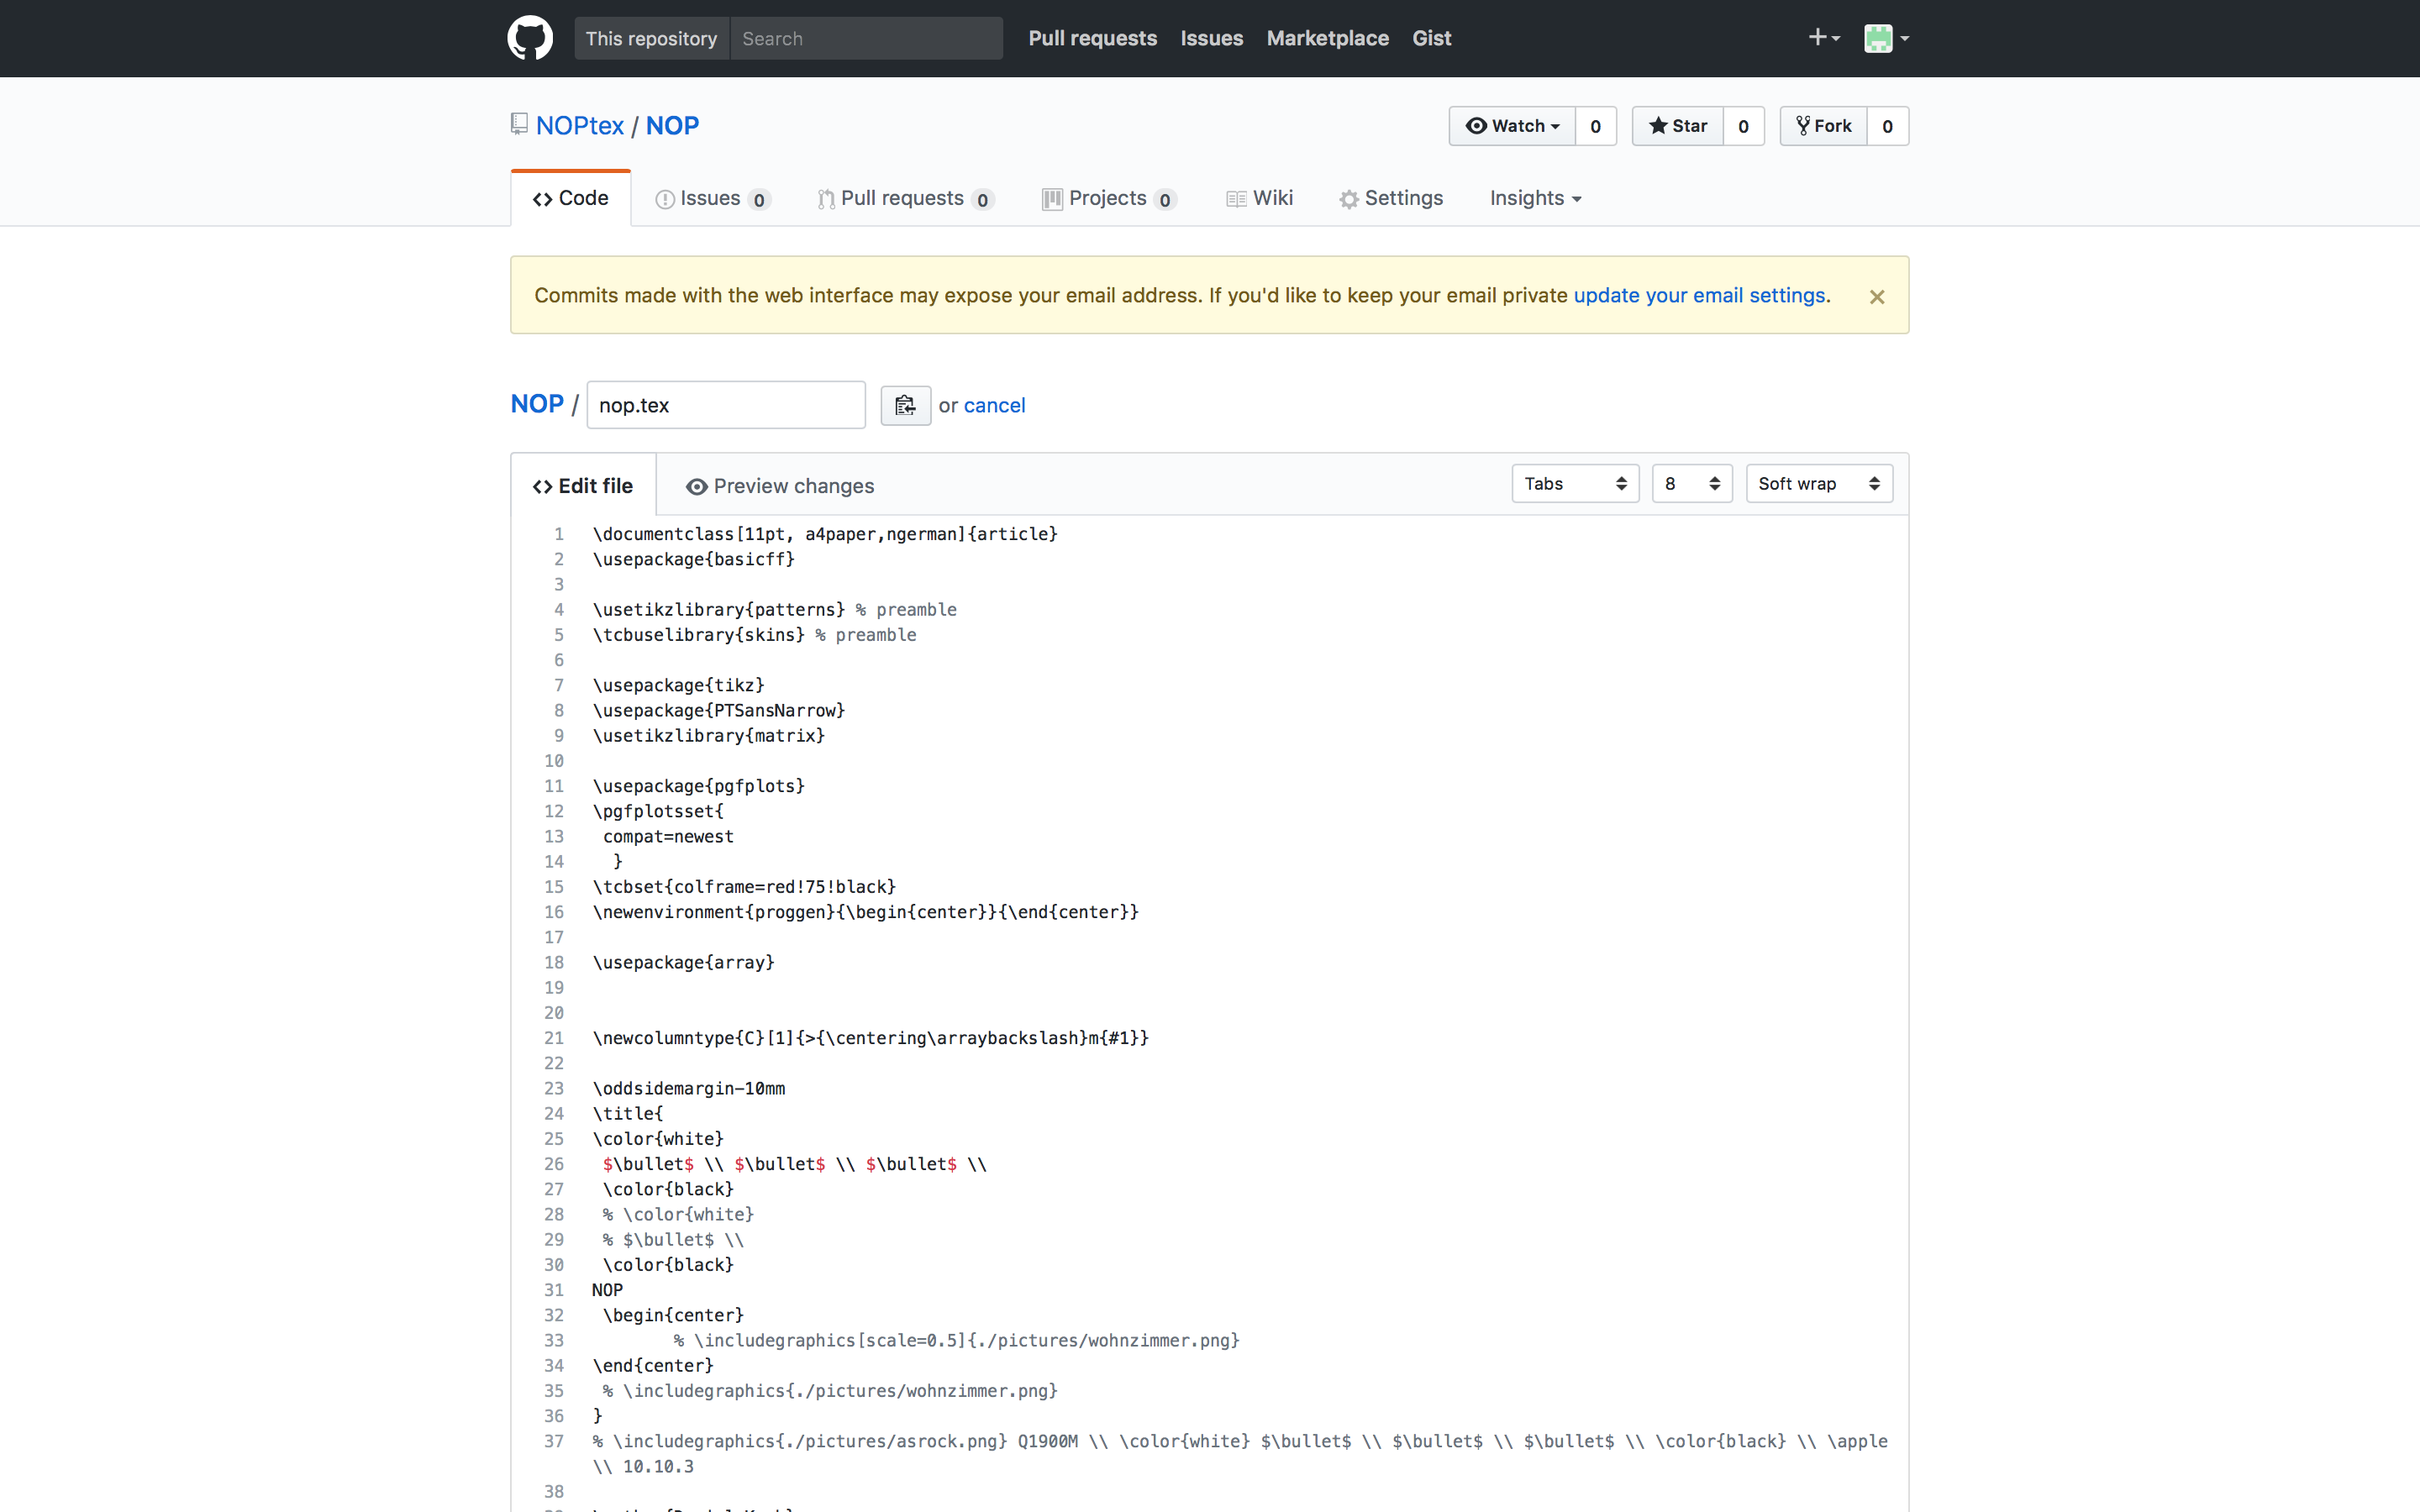
\includegraphics[width=1.0\textwidth]{./bilder/22edit.png}
\end{framed}

\end{minipage}}
\hfill
\adjustbox{valign=t}{\begin{minipage}[t]{0.45\textwidth}
\vspace{0pt}
\huge
Die Anzeige ändert sich geringfüging.
% \caption{Kapazität}
\end{minipage}}
\end{figure}

\clearpage % GleitObjekte anzeigen

\newpage % ============================================= Newpage ===================


\begin{figure}[ht]
  % \section{Release mit Tag erstellen und bauen}
\adjustbox{valign=t}{\begin{minipage}[t]{0.50\textwidth}
\begin{framed}
  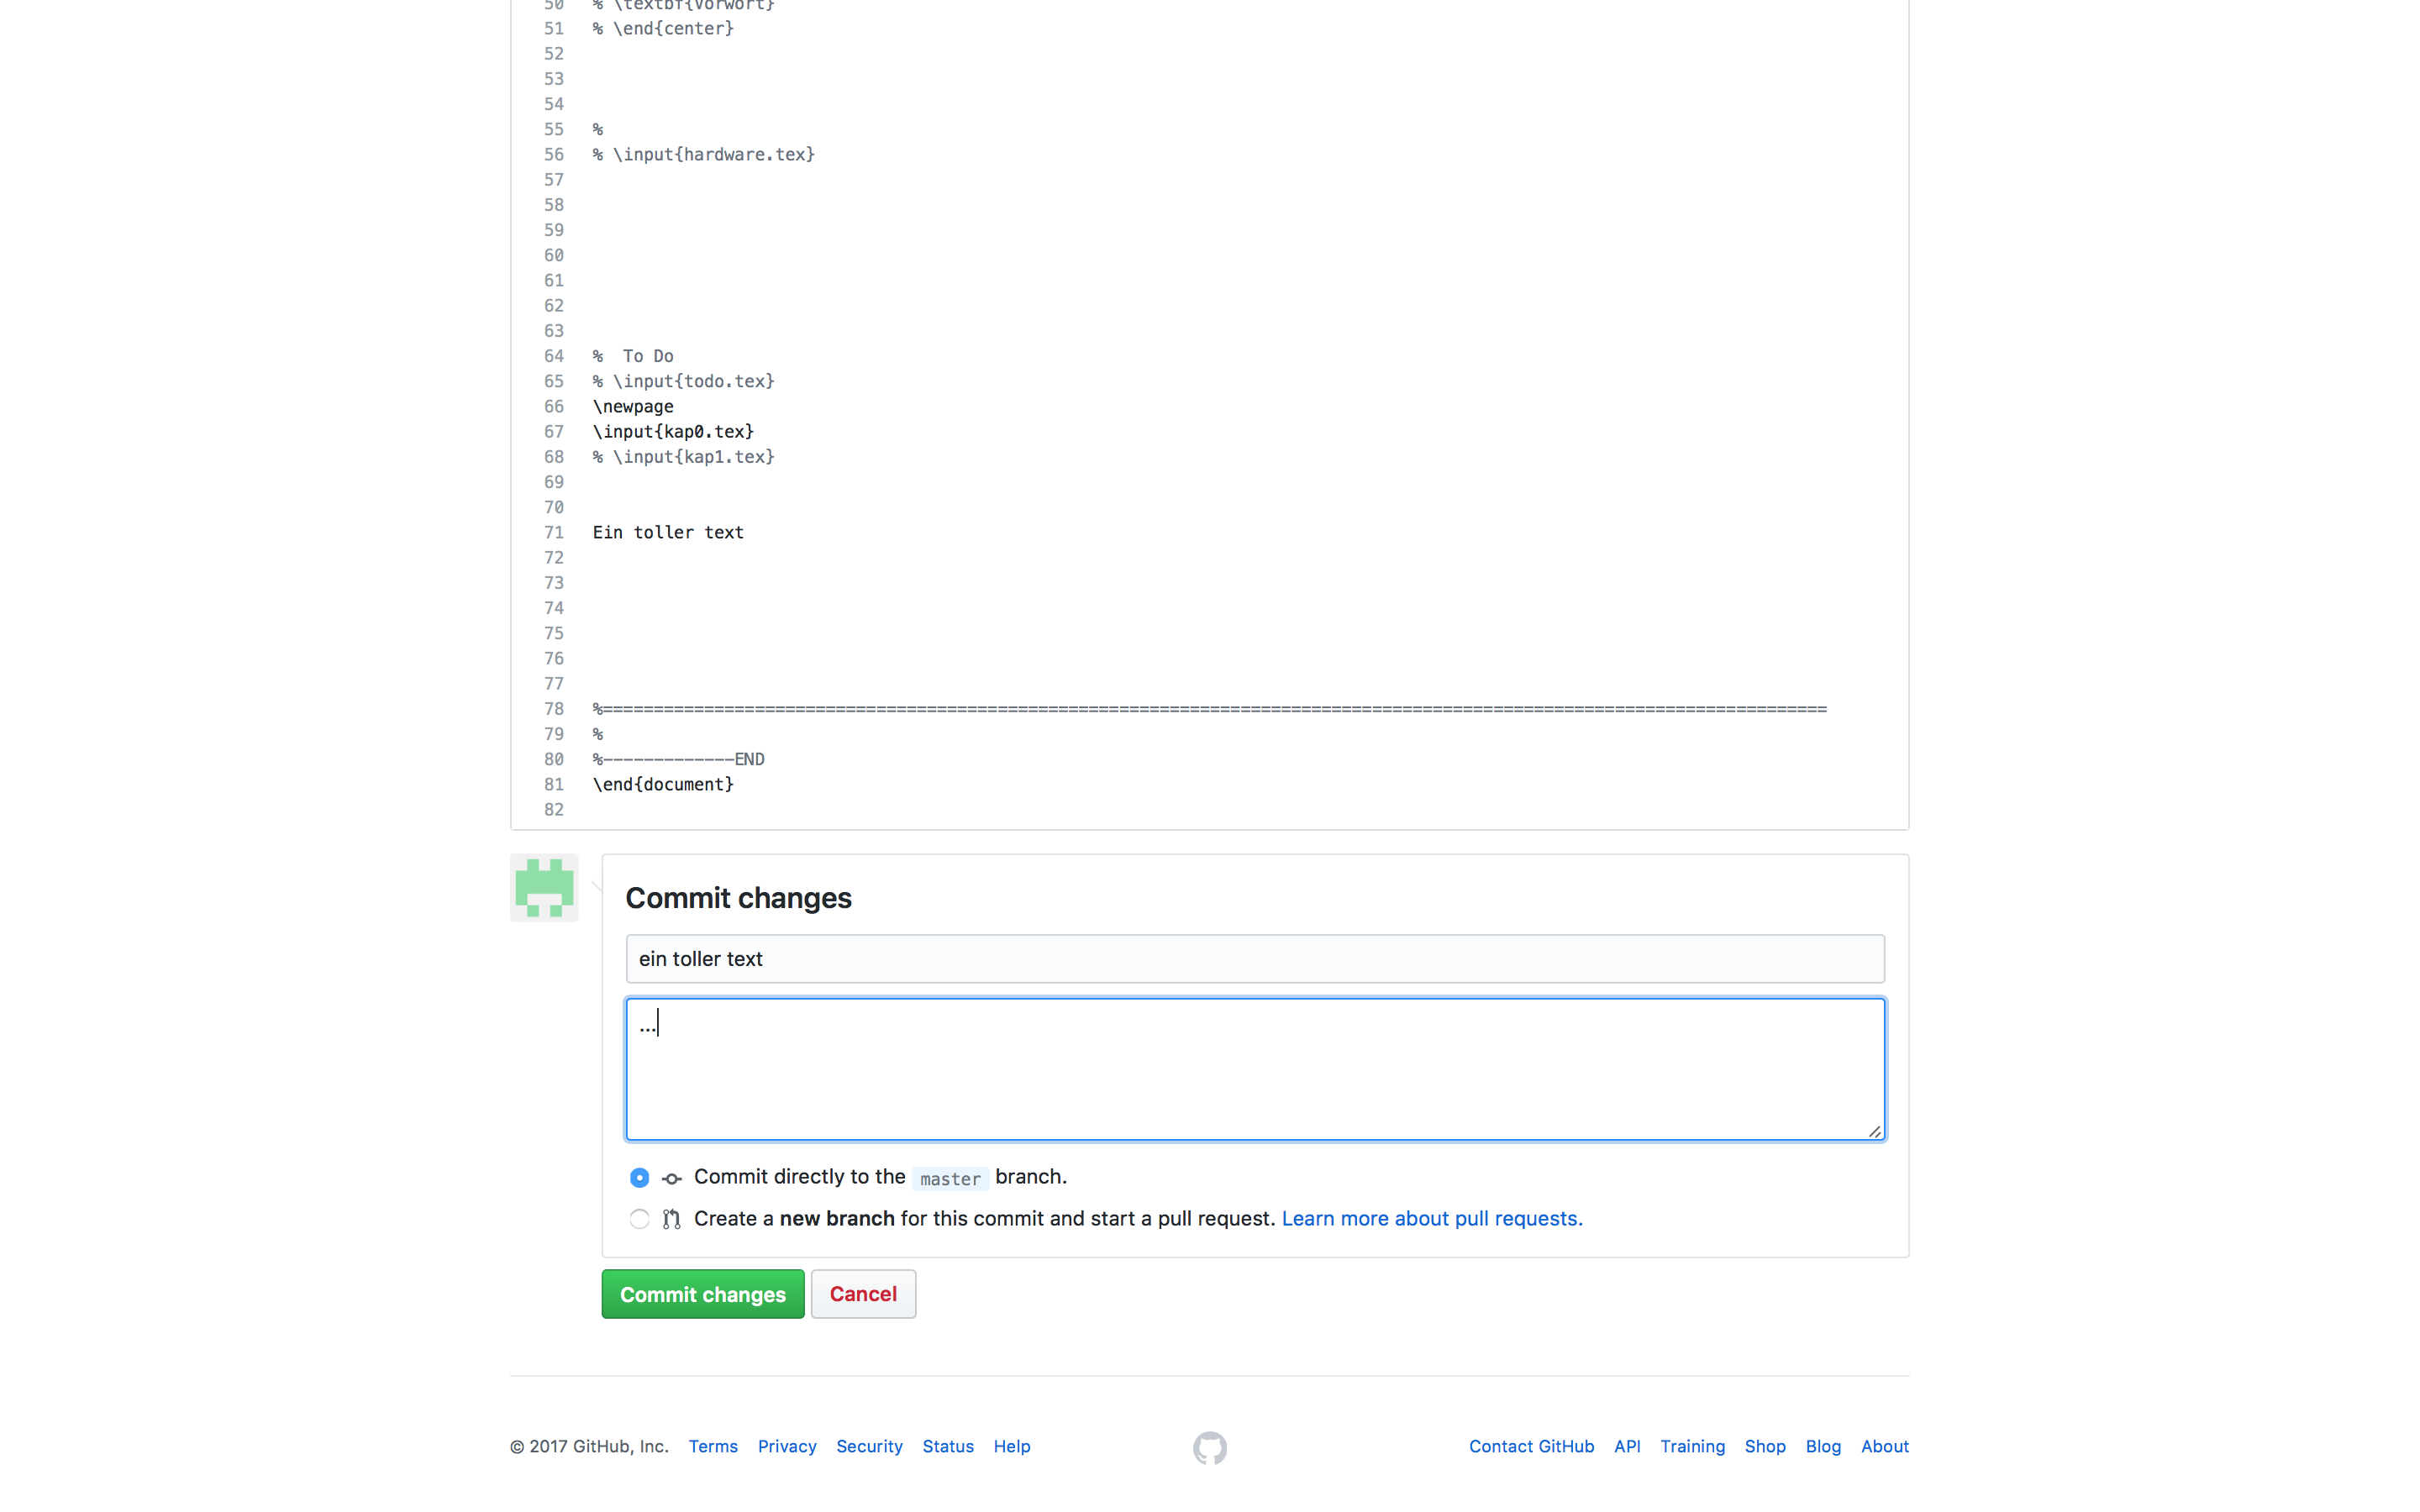
\includegraphics[width=1.0\textwidth]{./bilder/23createRelease.png}
\end{framed}

\end{minipage}}
% \hfill
\adjustbox{valign=t}{\begin{minipage}[t]{0.45\textwidth}
\vspace{0pt}
\huge
Text, Titel und Beschreibung hinzufügen.
% \caption{Kapazität}
\end{minipage}}
% \end{figure}
% \vspace{0.5cm} % ----------------------------------- vspace
% \begin{figure}[ht]
\adjustbox{valign=t}{\begin{minipage}[t]{0.50\textwidth}
% \vspace{0.5cm}
\begin{framed}
  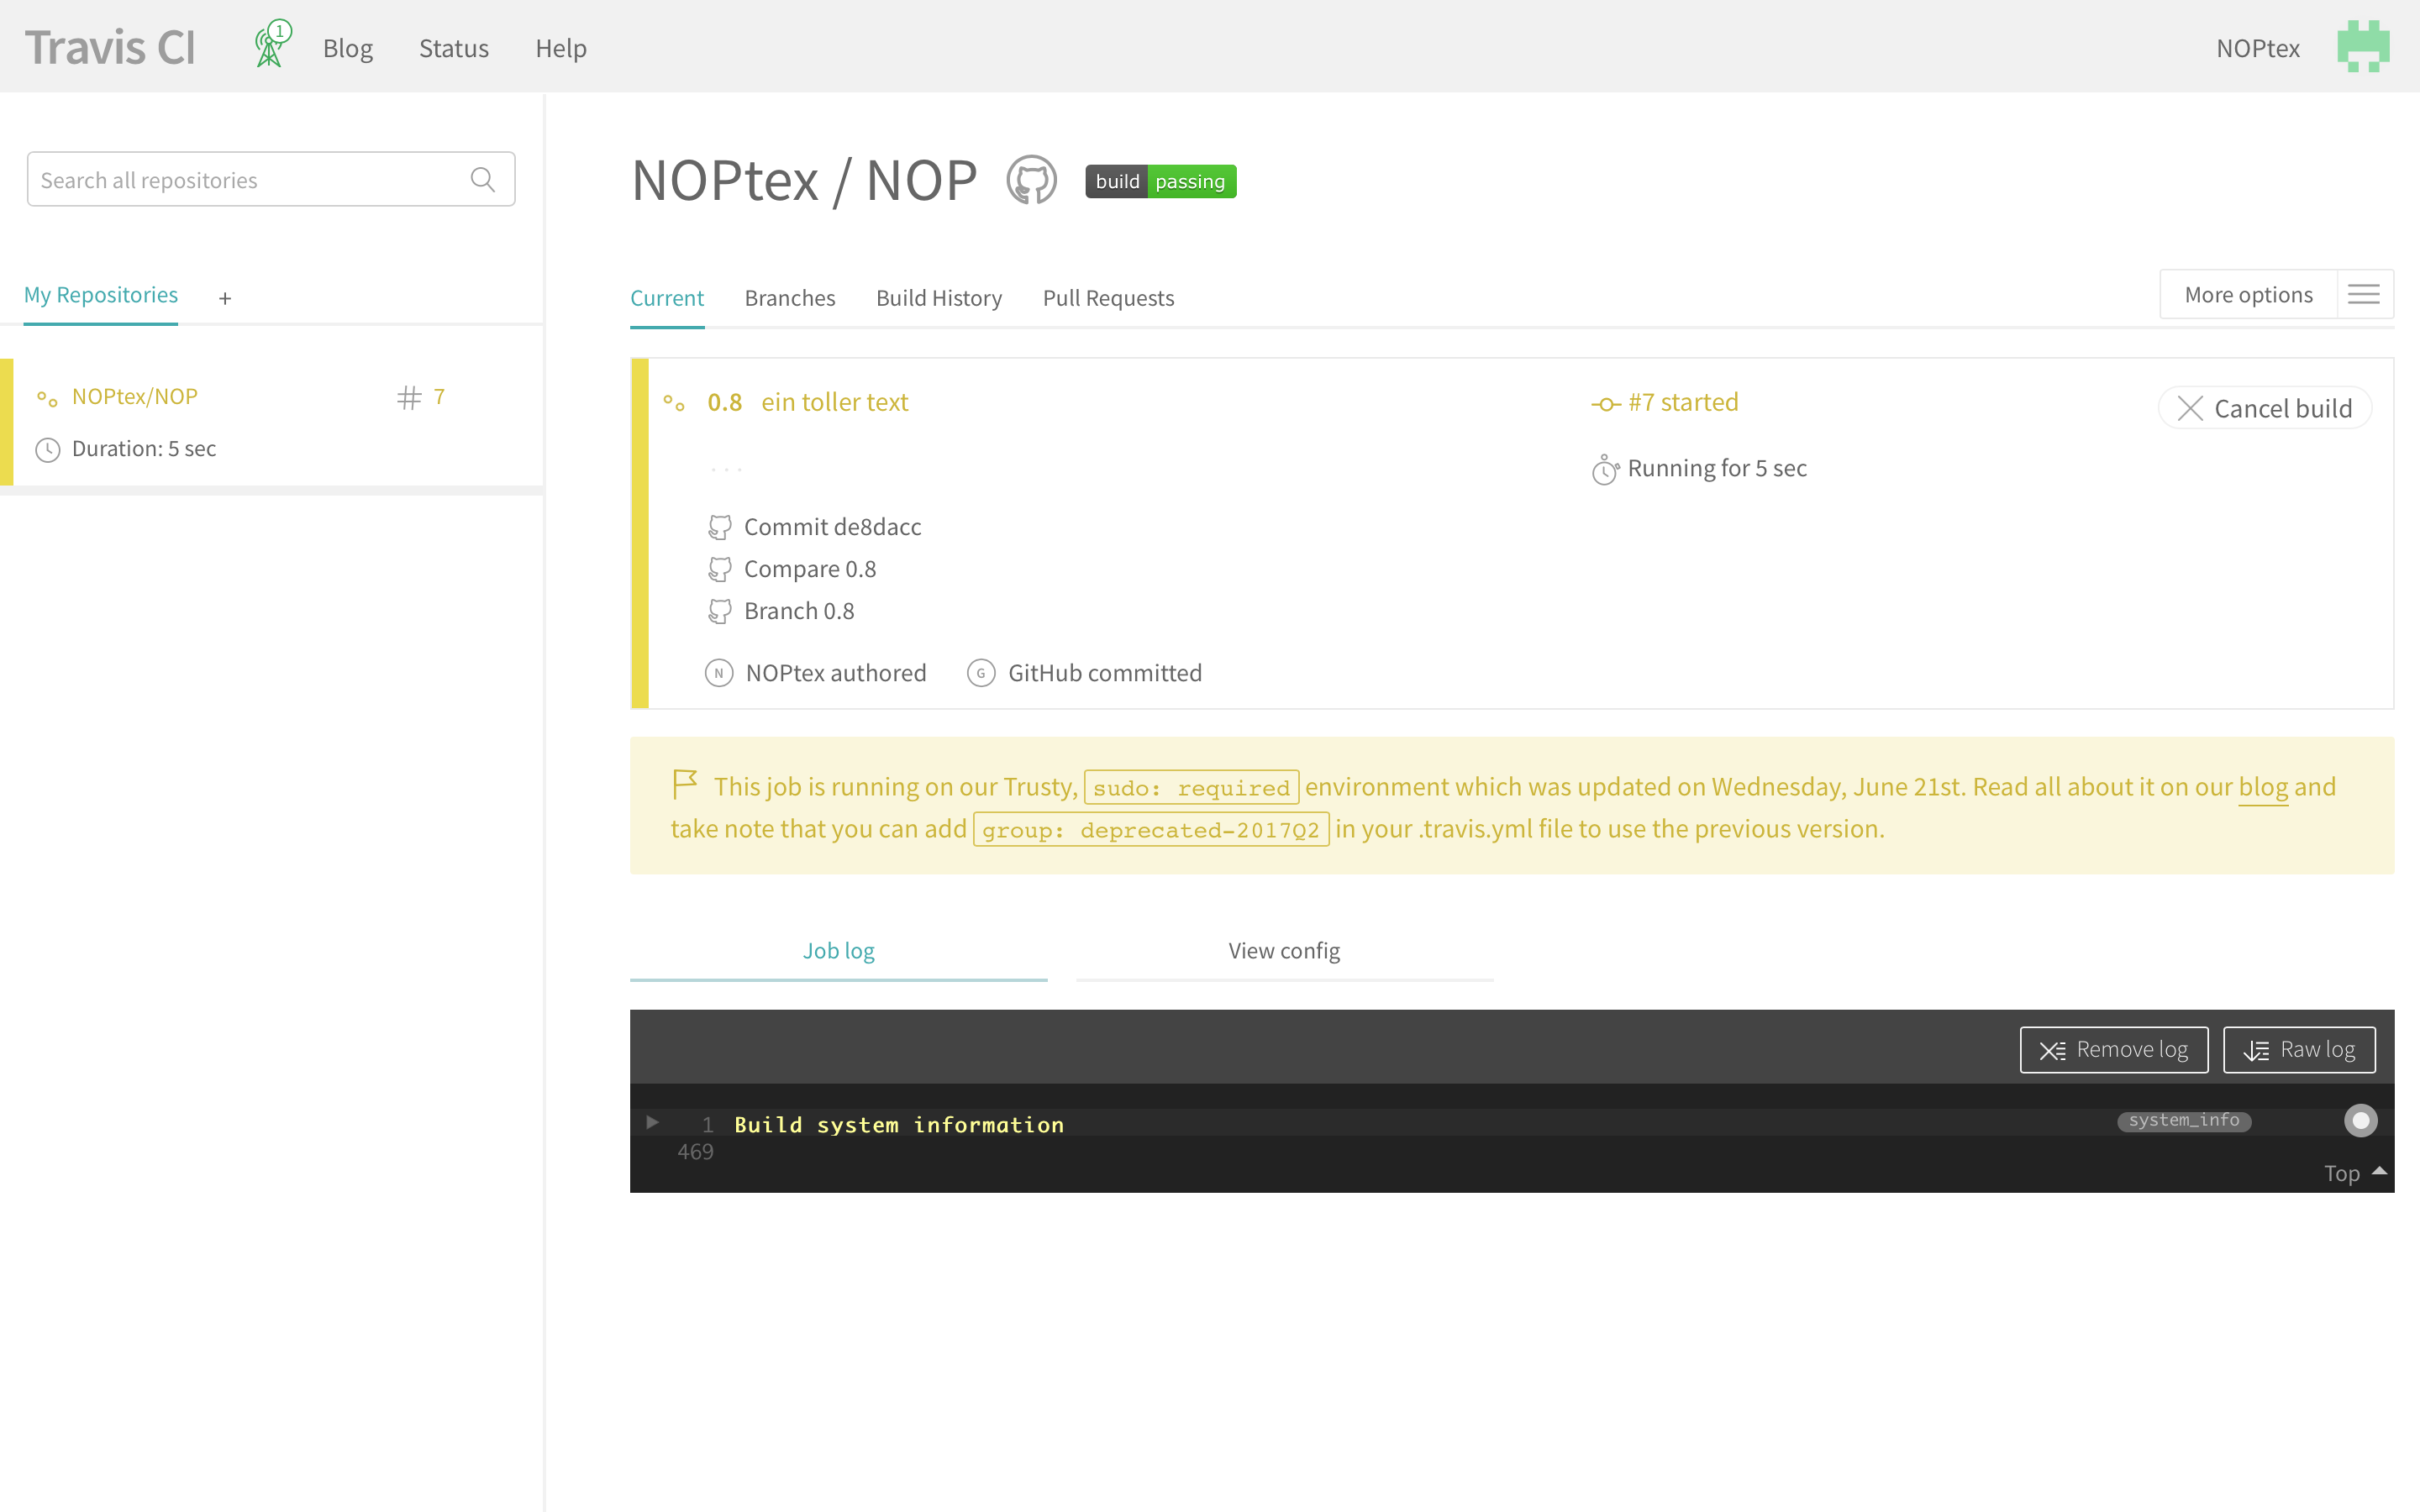
\includegraphics[width=1.0\textwidth]{./bilder/24baut.png}
\end{framed}

\end{minipage}}
\hfill
\adjustbox{valign=t}{\begin{minipage}[t]{0.45\textwidth}
\vspace{0pt}
\huge
Kontrolle bei Travis und es baut.\\
(Das dauert dann so 7-8 Minuten.)
% \caption{Kapazität}
\end{minipage}}
\end{figure}

\clearpage % GleitObjekte anzeigen


\newpage % ============================================= Newpage ===================


\begin{figure}[ht]
  \section{Erfolgreich gebaut}
\adjustbox{valign=t}{\begin{minipage}[t]{0.50\textwidth}
\begin{framed}
  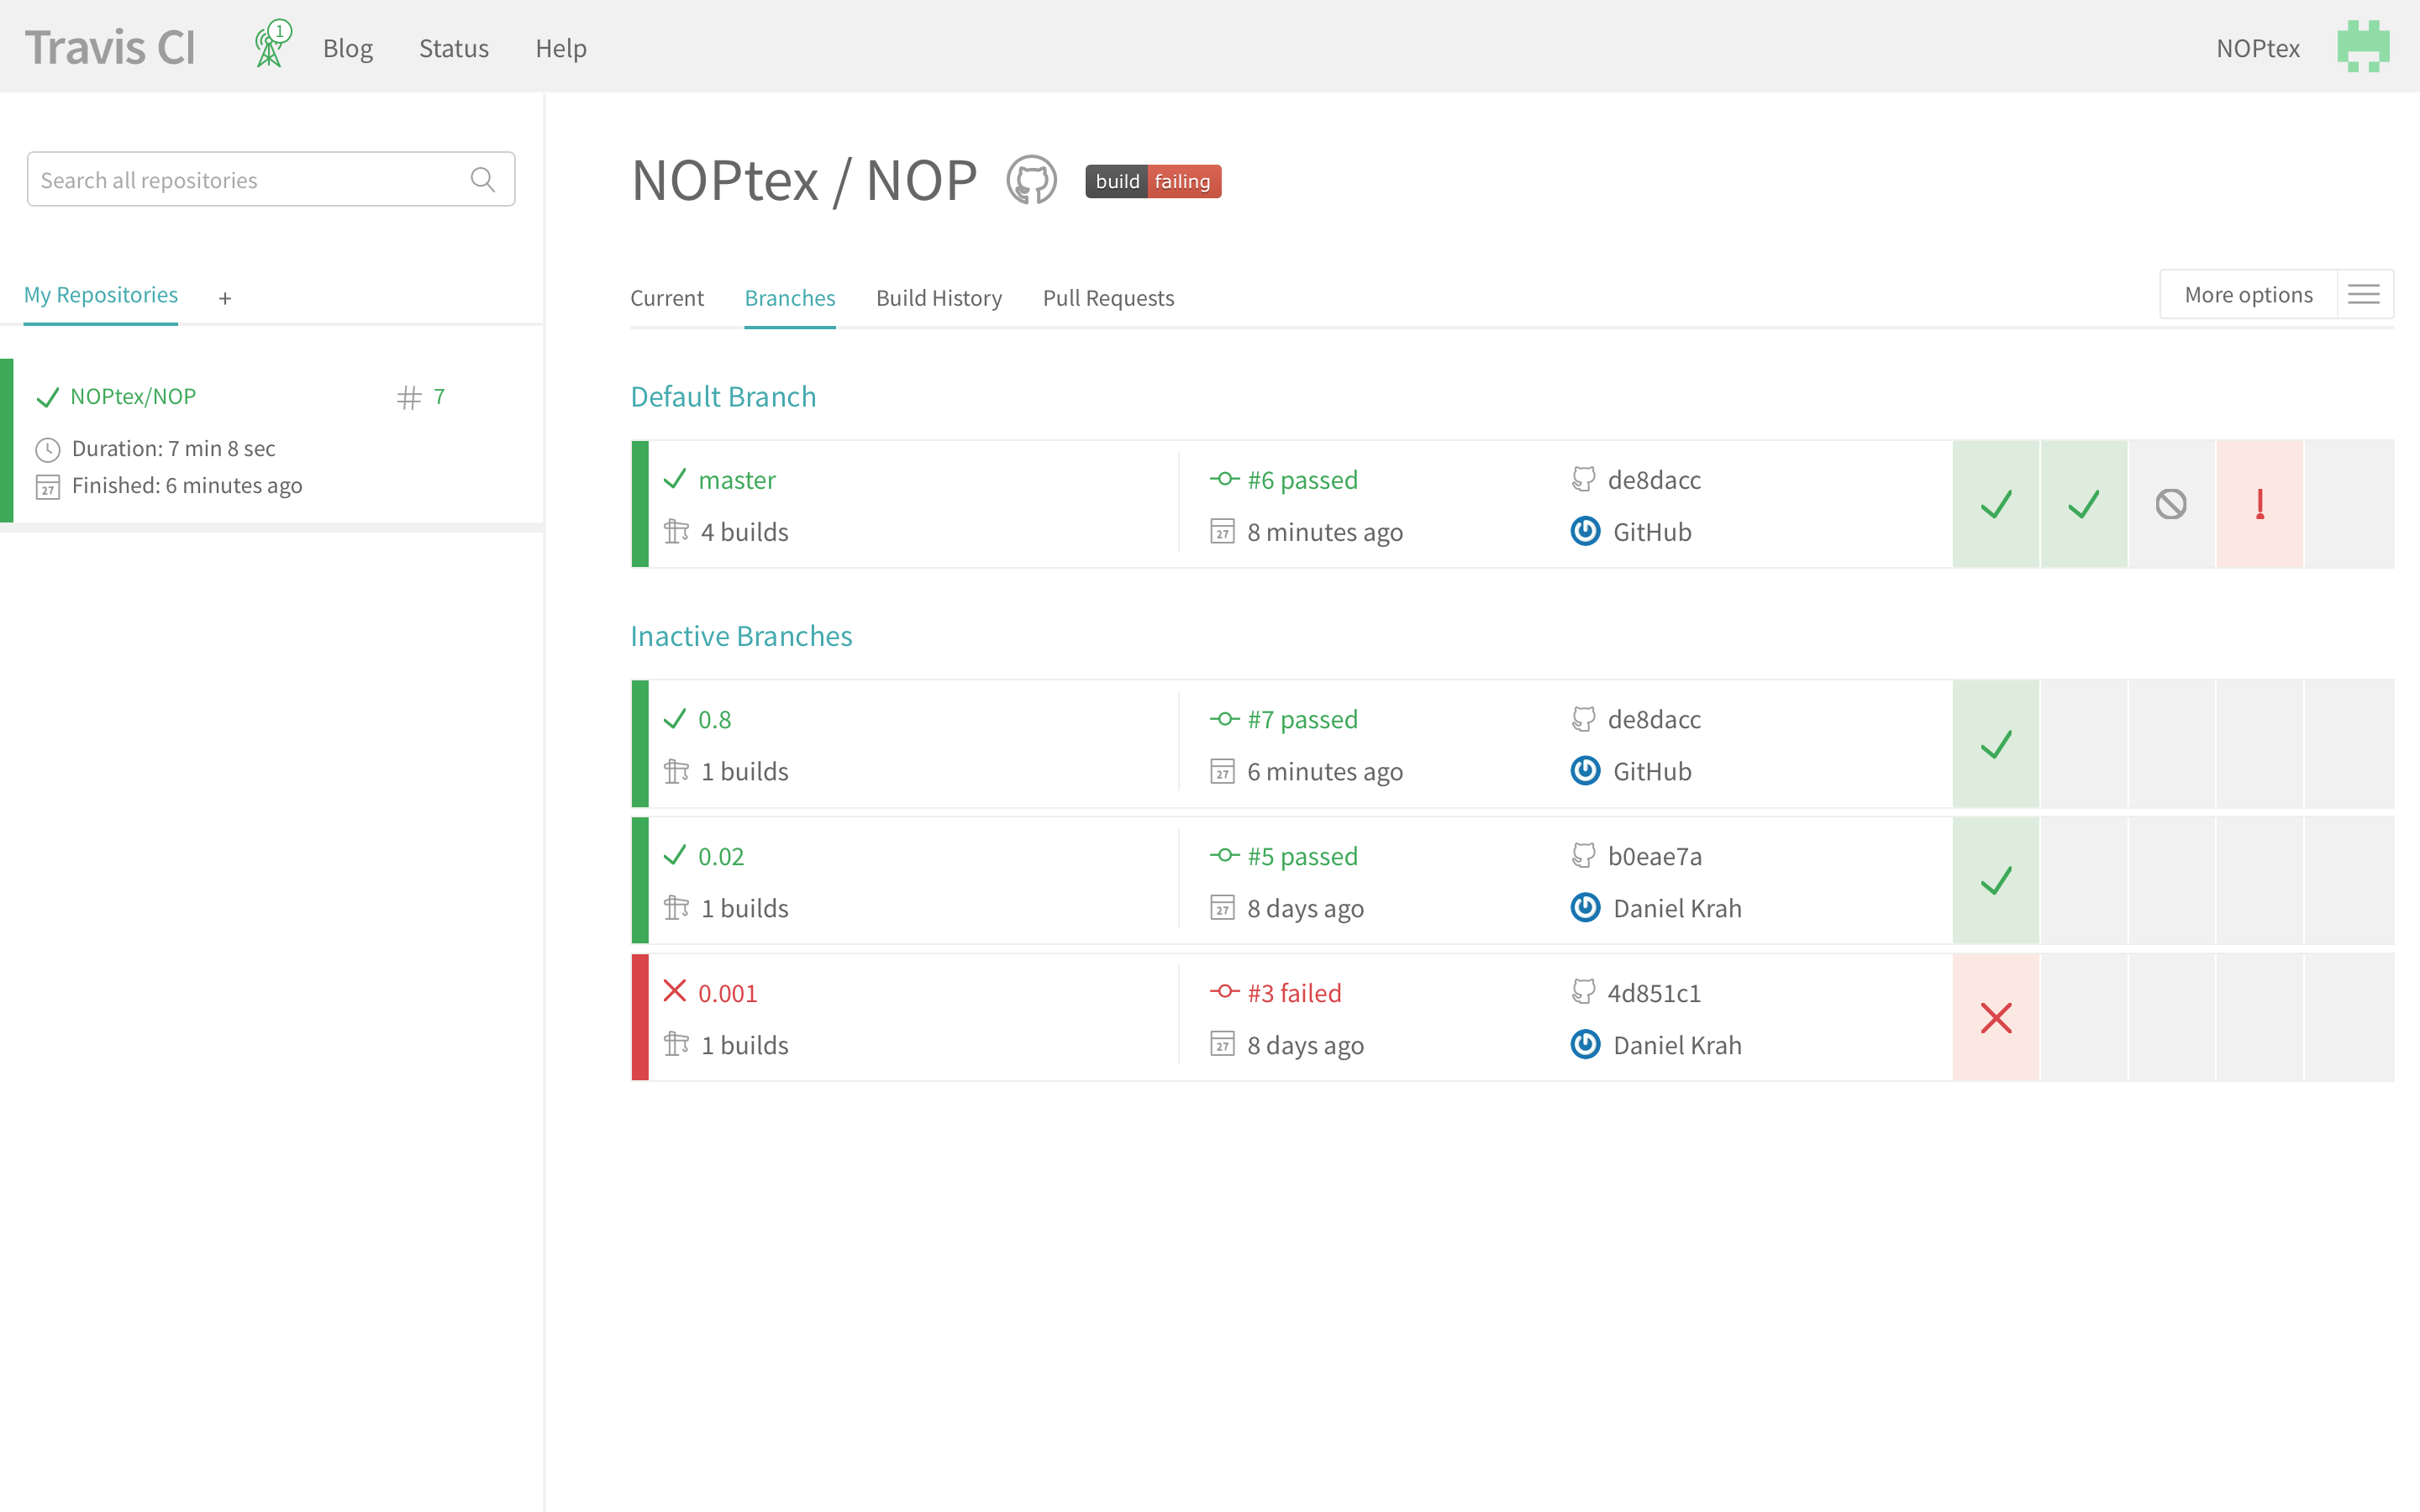
\includegraphics[width=1.0\textwidth]{./bilder/25gebaut.png}
\end{framed}

\end{minipage}}
% \hfill
\adjustbox{valign=t}{\begin{minipage}[t]{0.45\textwidth}
\vspace{0pt}
\huge
Wenn fertig sieht es so aus.
% \caption{Kapazität}
\end{minipage}}
% \end{figure}
% \vspace{0.5cm} % ----------------------------------- vspace
% \begin{figure}[ht]
\adjustbox{valign=t}{\begin{minipage}[t]{0.50\textwidth}
% \vspace{0.5cm}
\begin{framed}
  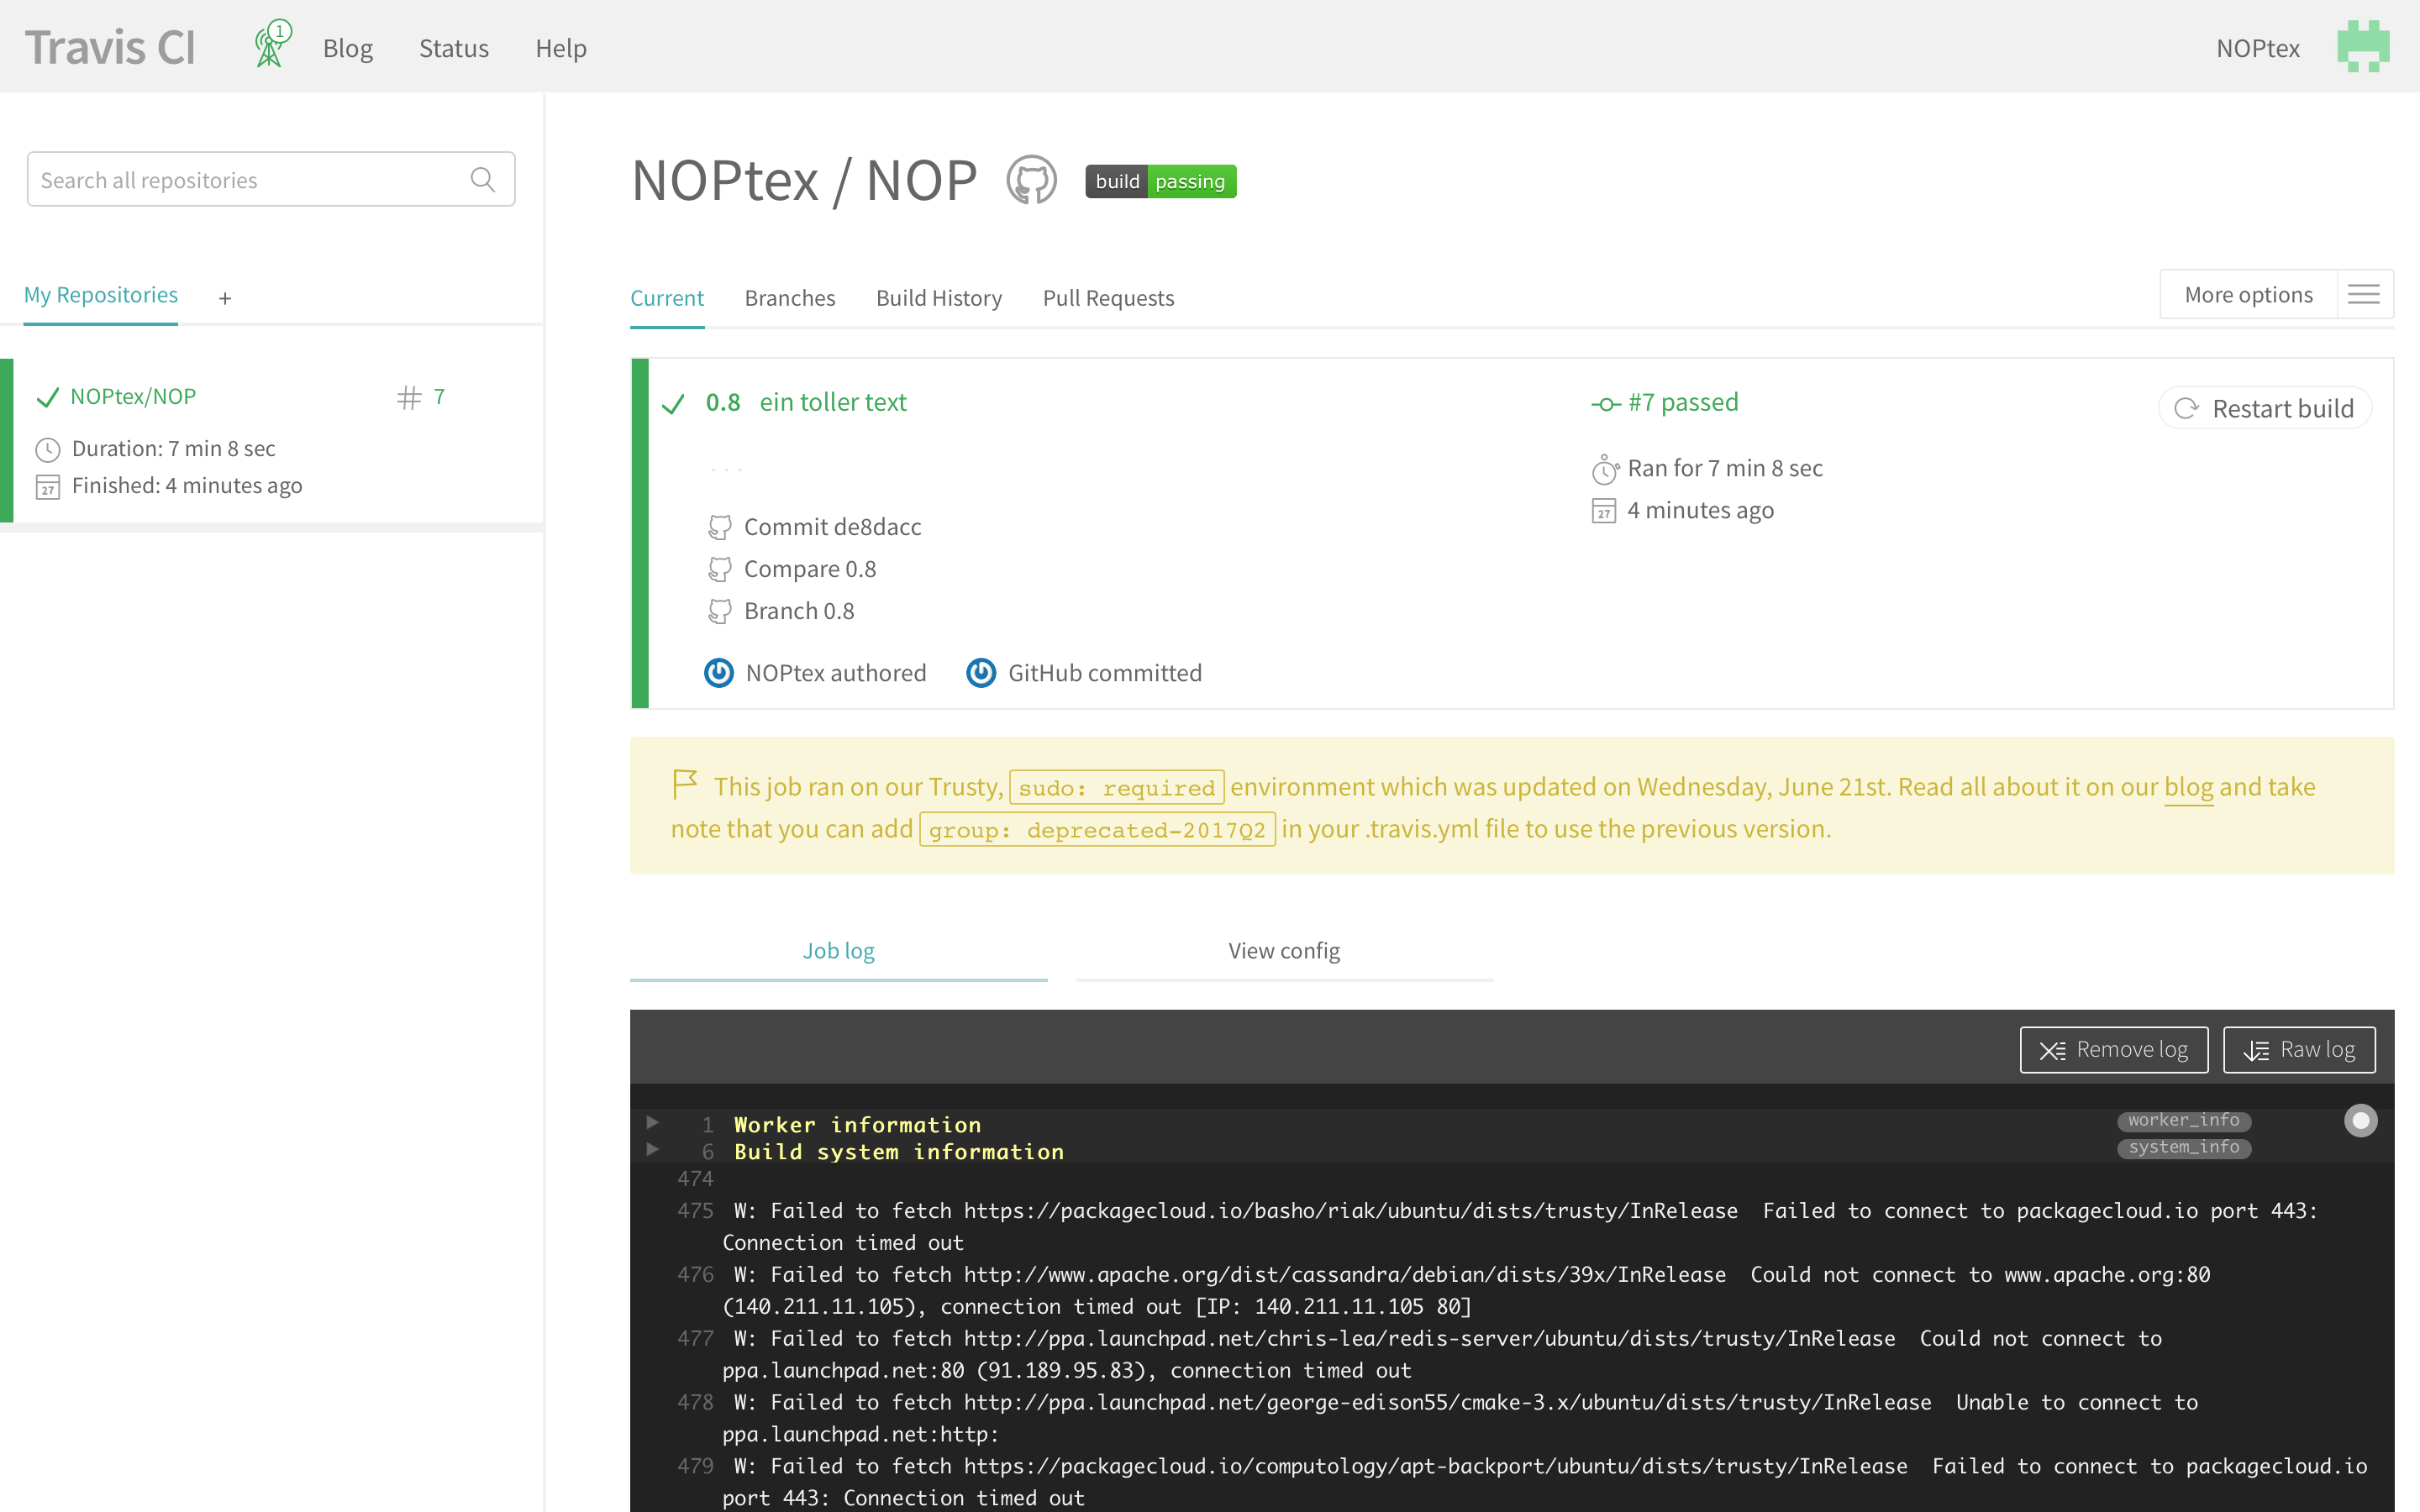
\includegraphics[width=1.0\textwidth]{./bilder/26details.png}
\end{framed}

\end{minipage}}
\hfill
\adjustbox{valign=t}{\begin{minipage}[t]{0.45\textwidth}
\vspace{0pt}
\huge
Optional kann man die Log-Ausgaben anschauen. \\
Aber in diesem Fall ging ja alles gut.
% \caption{Kapazität}
\end{minipage}}
\end{figure}

\clearpage % GleitObjekte anzeigen

\newpage % ============================================= Newpage ===================


\begin{figure}[ht]
  \section{Github kontrollieren und PDF überprüfen}
\adjustbox{valign=t}{\begin{minipage}[t]{0.50\textwidth}
\begin{framed}
  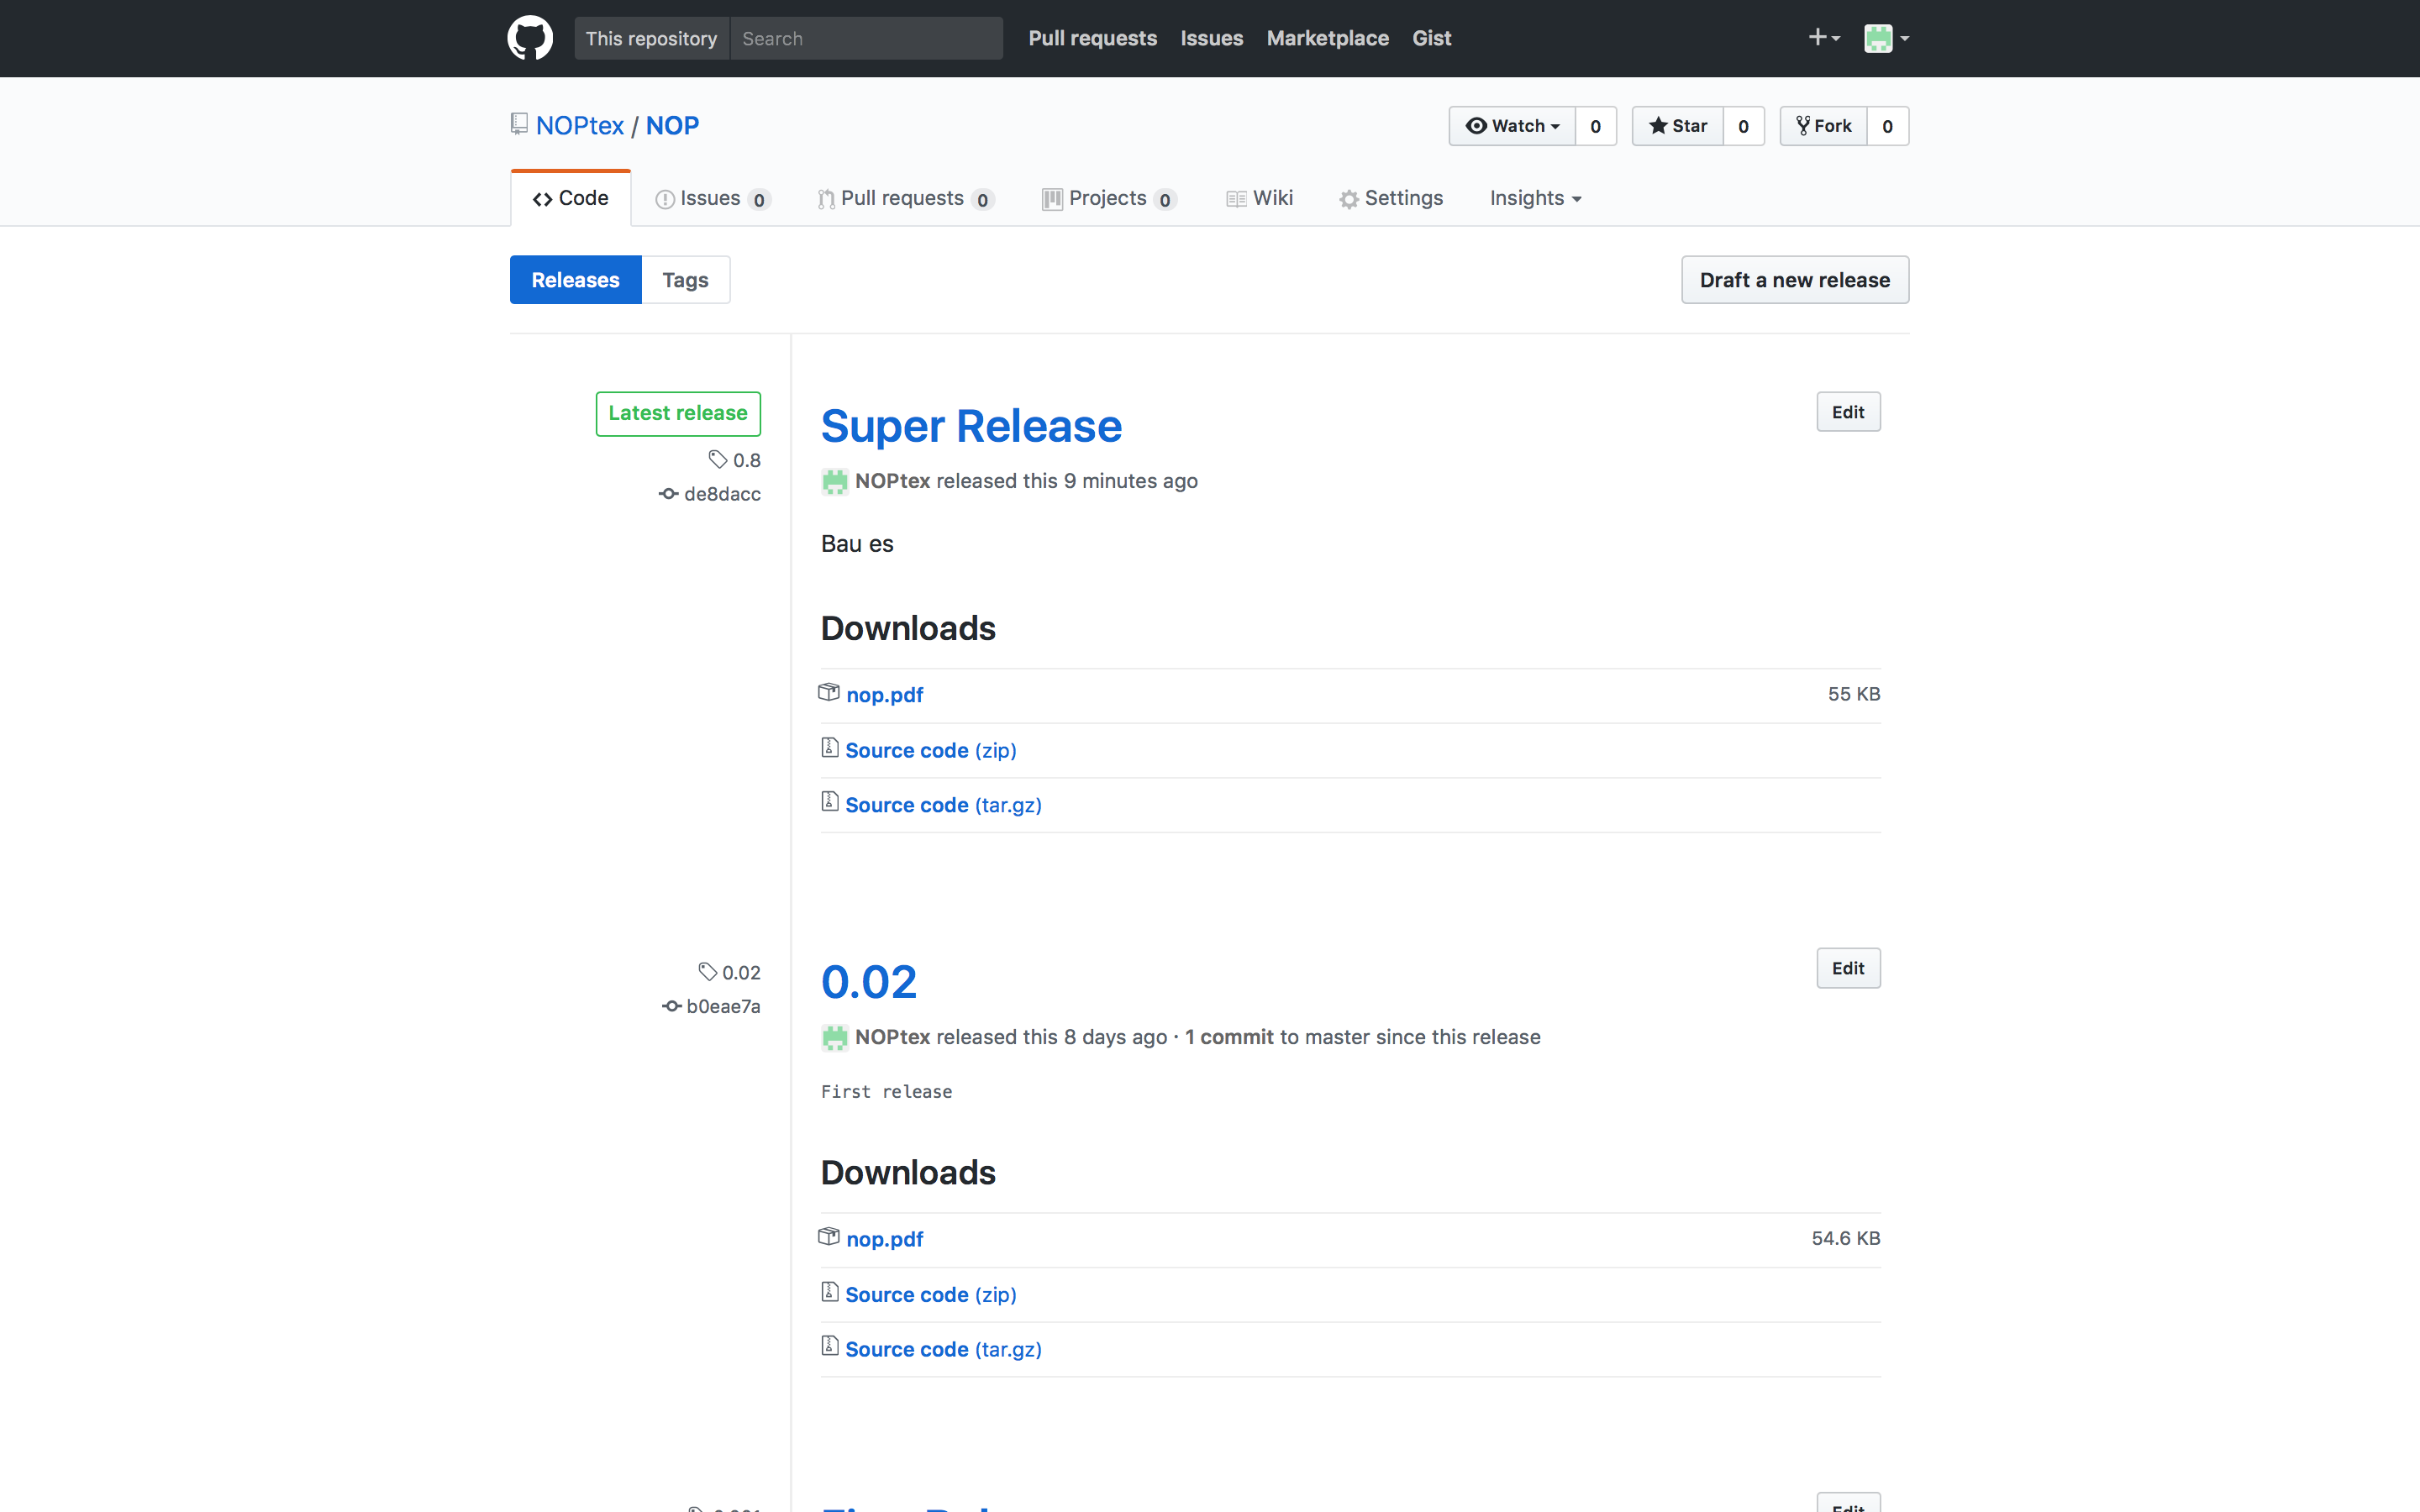
\includegraphics[width=1.0\textwidth]{./bilder/27release.png}
\end{framed}

\end{minipage}}
% \hfill
\adjustbox{valign=t}{\begin{minipage}[t]{0.45\textwidth}
\vspace{0pt}
\huge
Auf GitHub ist nun auch die PDF under Releases ...
% \caption{Kapazität}
\end{minipage}}
% \end{figure}
% \vspace{0.5cm} % ----------------------------------- vspace
% \begin{figure}[ht]
\adjustbox{valign=t}{\begin{minipage}[t]{0.50\textwidth}
% \vspace{0.5cm}
\begin{framed}
  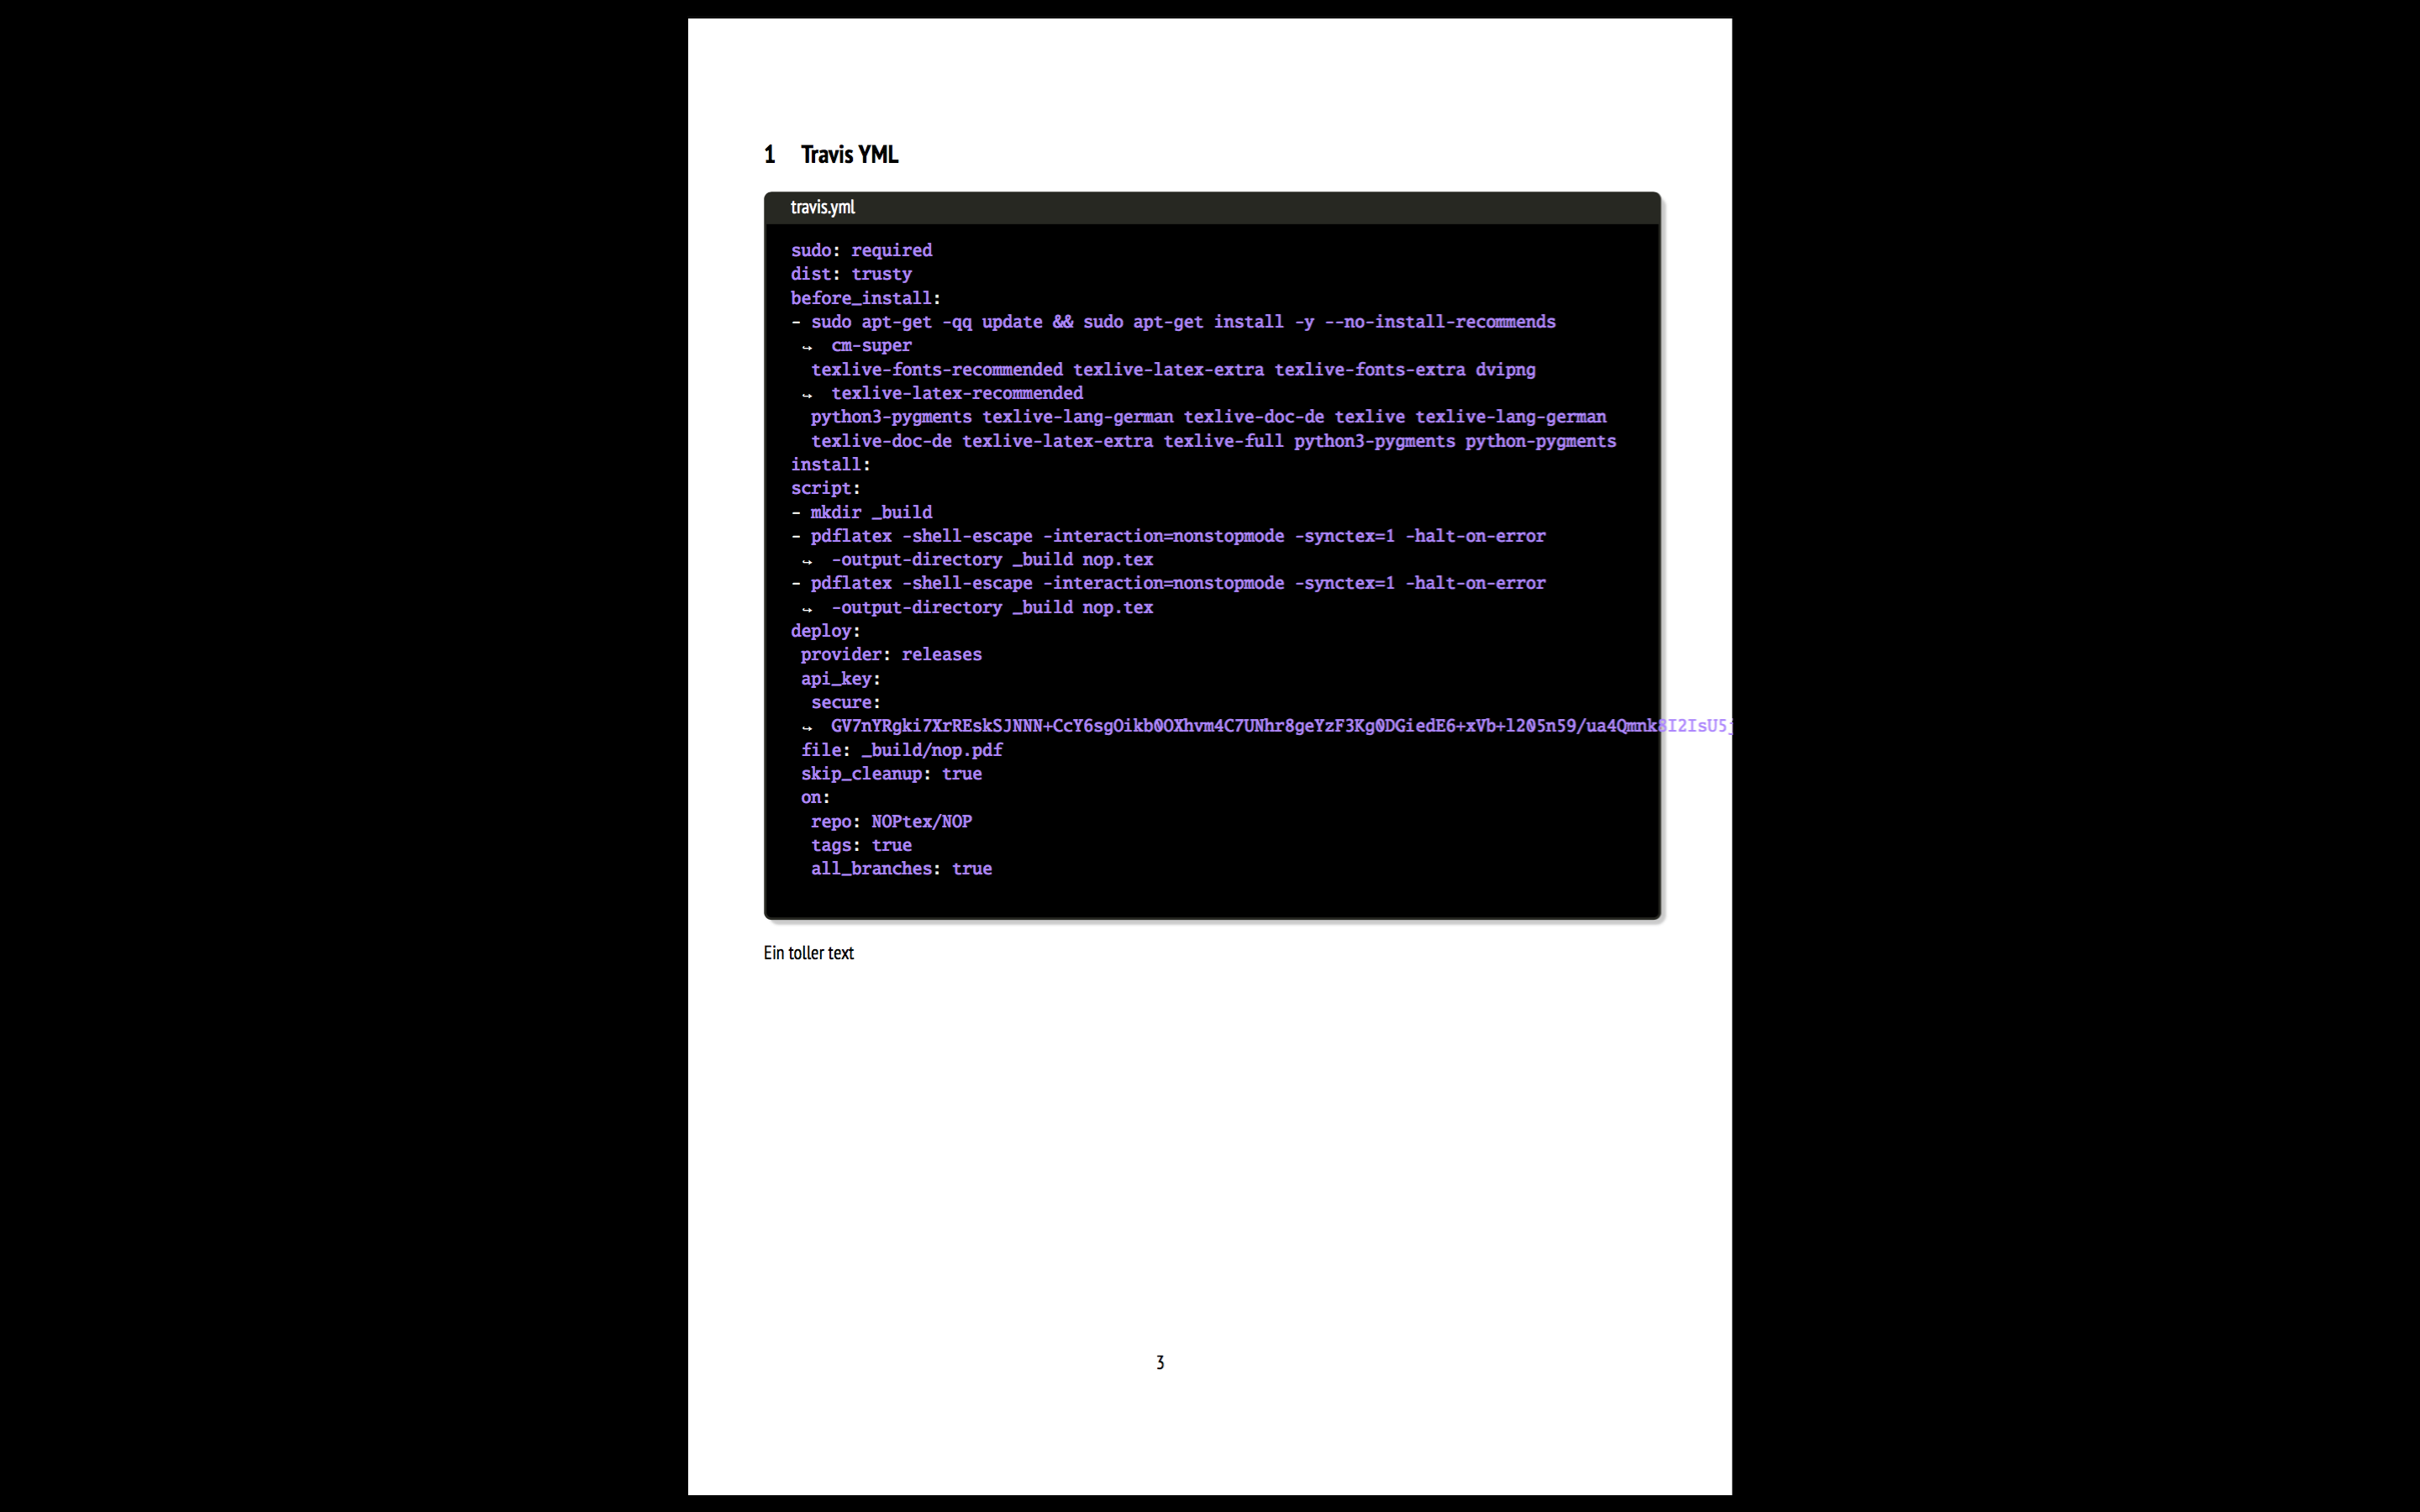
\includegraphics[width=1.0\textwidth]{./bilder/28fertig.png}
\end{framed}

\end{minipage}}
\hfill
\adjustbox{valign=t}{\begin{minipage}[t]{0.45\textwidth}
\vspace{0pt}
\huge
PDF sieht gut aus und die Änderung ist mit drinnen.
% \caption{Kapazität}
\end{minipage}}
\end{figure}

\clearpage % GleitObjekte anzeigen
    % travis yml
\newpage

\section{Github + Travis CI mittels arara + luatex}
\subsection{aktuelle Probleme}
\subsubsection{Linux}
\begin{itemize}
  \item Travis CI verwende eine sehr alte Ubuntu-Version.\\ (Dadurch nur eine veraltete TexLive installation\\ $\Rightarrow$ hinderlich bei Lua\TeX)
  \item Aktuell verfügbare Docker-Container bekommen \\das Texlive Update nicht hin.
  \item Arara bekommt generell keine Rechte um die Dateien zu schreiben. \\
  (Evtl. lösbar, aber die Zeit ist grade knapp)
\end{itemize}

\newpage
$\Rightarrow$ aktuelle Probleme
\subsubsection{MacOS 10}
\begin{itemize}
  \item Unter OSX dauert die Latex Installation zu lange. \\ $\Rightarrow$ Travis CI bricht ab ...
  \item Docker-Nutzung schwierig, da man dafür Virtualbox + ein Linux benötigt.
  \item Brew (Ein Paketmanager für MacOS) enthält kein Tex-Live.
  \item Macports (nicht in den TravisCI - macOS10-Installationen enthalten)
\end{itemize}


\newpage % ============================================= Newpage ===================

\monocodebox{latex}{Was benötigt es für arara:}{./nopTex.tex}{true}{1}{3}

\monocodebox{sh}{Hinzufuegen der nötigen Änderungen}{./code/travis.sh}{true}{80}{80}







%
% \begin{figure}[ht]
%   \section{arara + lua \TeX}
% \adjustbox{valign=t}{\begin{minipage}[t]{0.50\textwidth}
% \begin{framed}
%   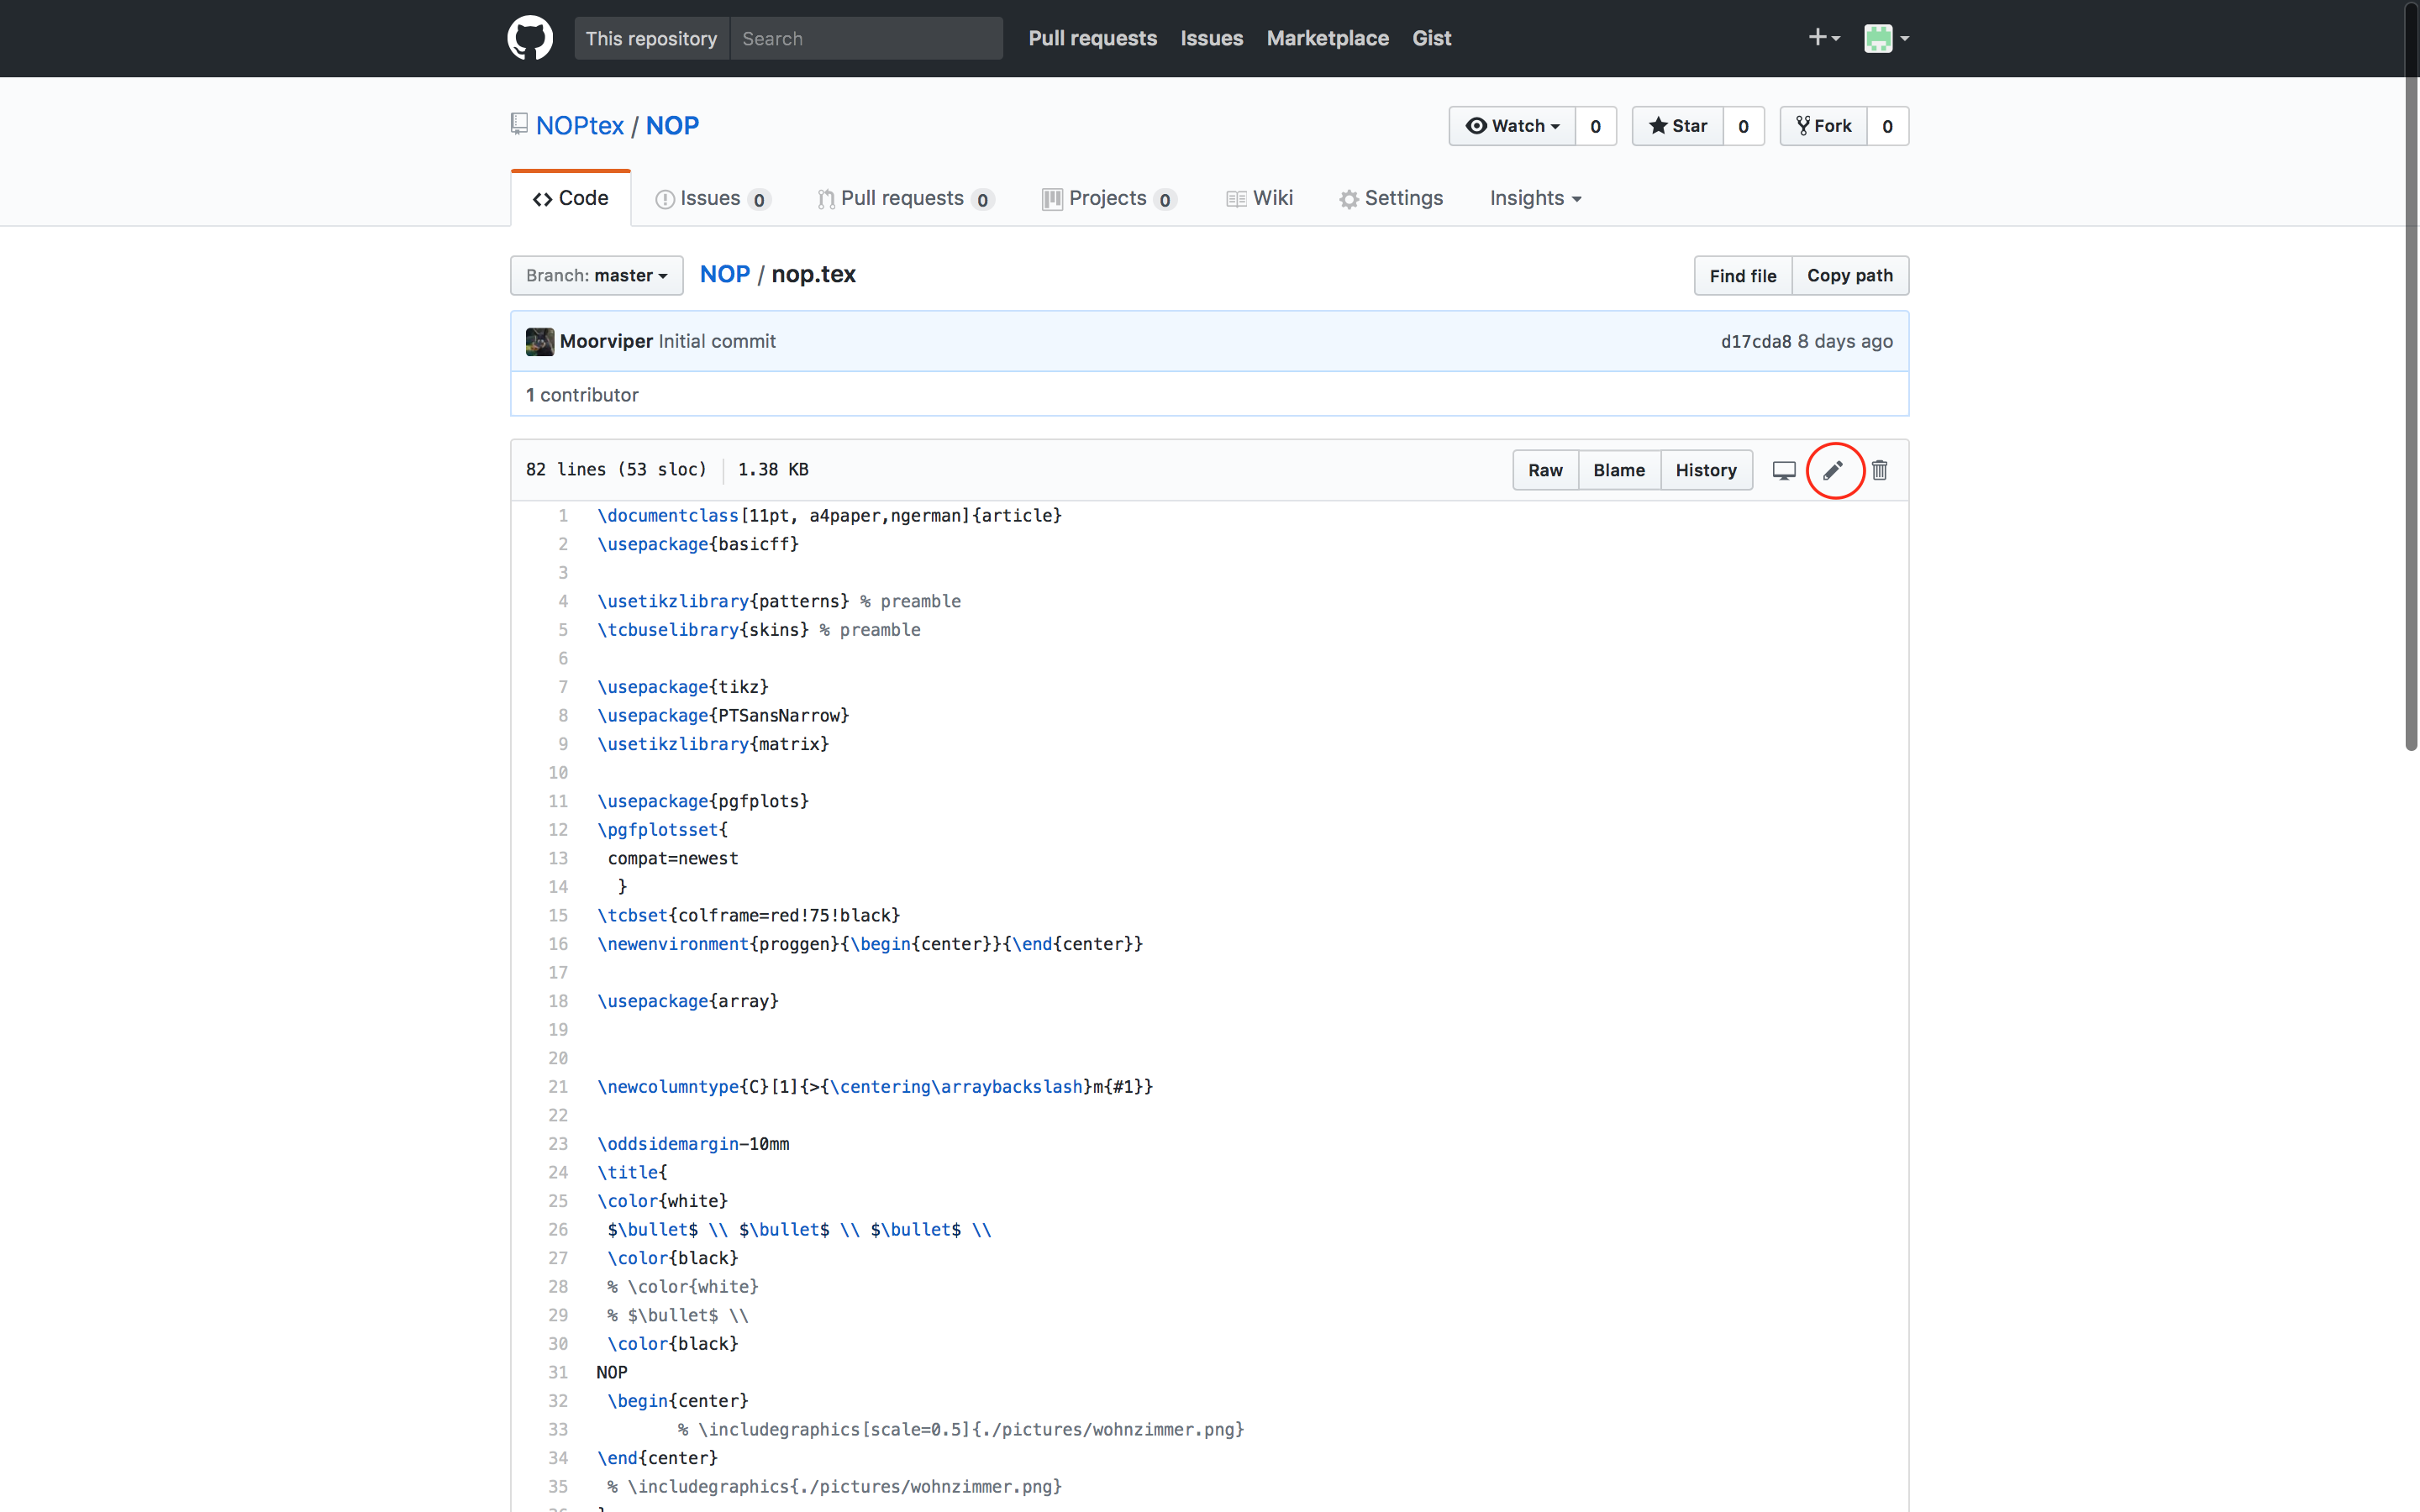
\includegraphics[width=1.0\textwidth]{./bilder/21edit.png}
% \end{framed}
%
% \end{minipage}}
% % \hfill
% \adjustbox{valign=t}{\begin{minipage}[t]{0.45\textwidth}
% \vspace{0pt}
% \huge
% Man klickt auf den Stift zum editieren der Datei.
% % \caption{Kapazität}
% \end{minipage}}
% % \end{figure}
% % \vspace{0.5cm} % ----------------------------------- vspace
% % \begin{figure}[ht]
% \adjustbox{valign=t}{\begin{minipage}[t]{0.50\textwidth}
% % \vspace{0.5cm}
% \begin{framed}
%   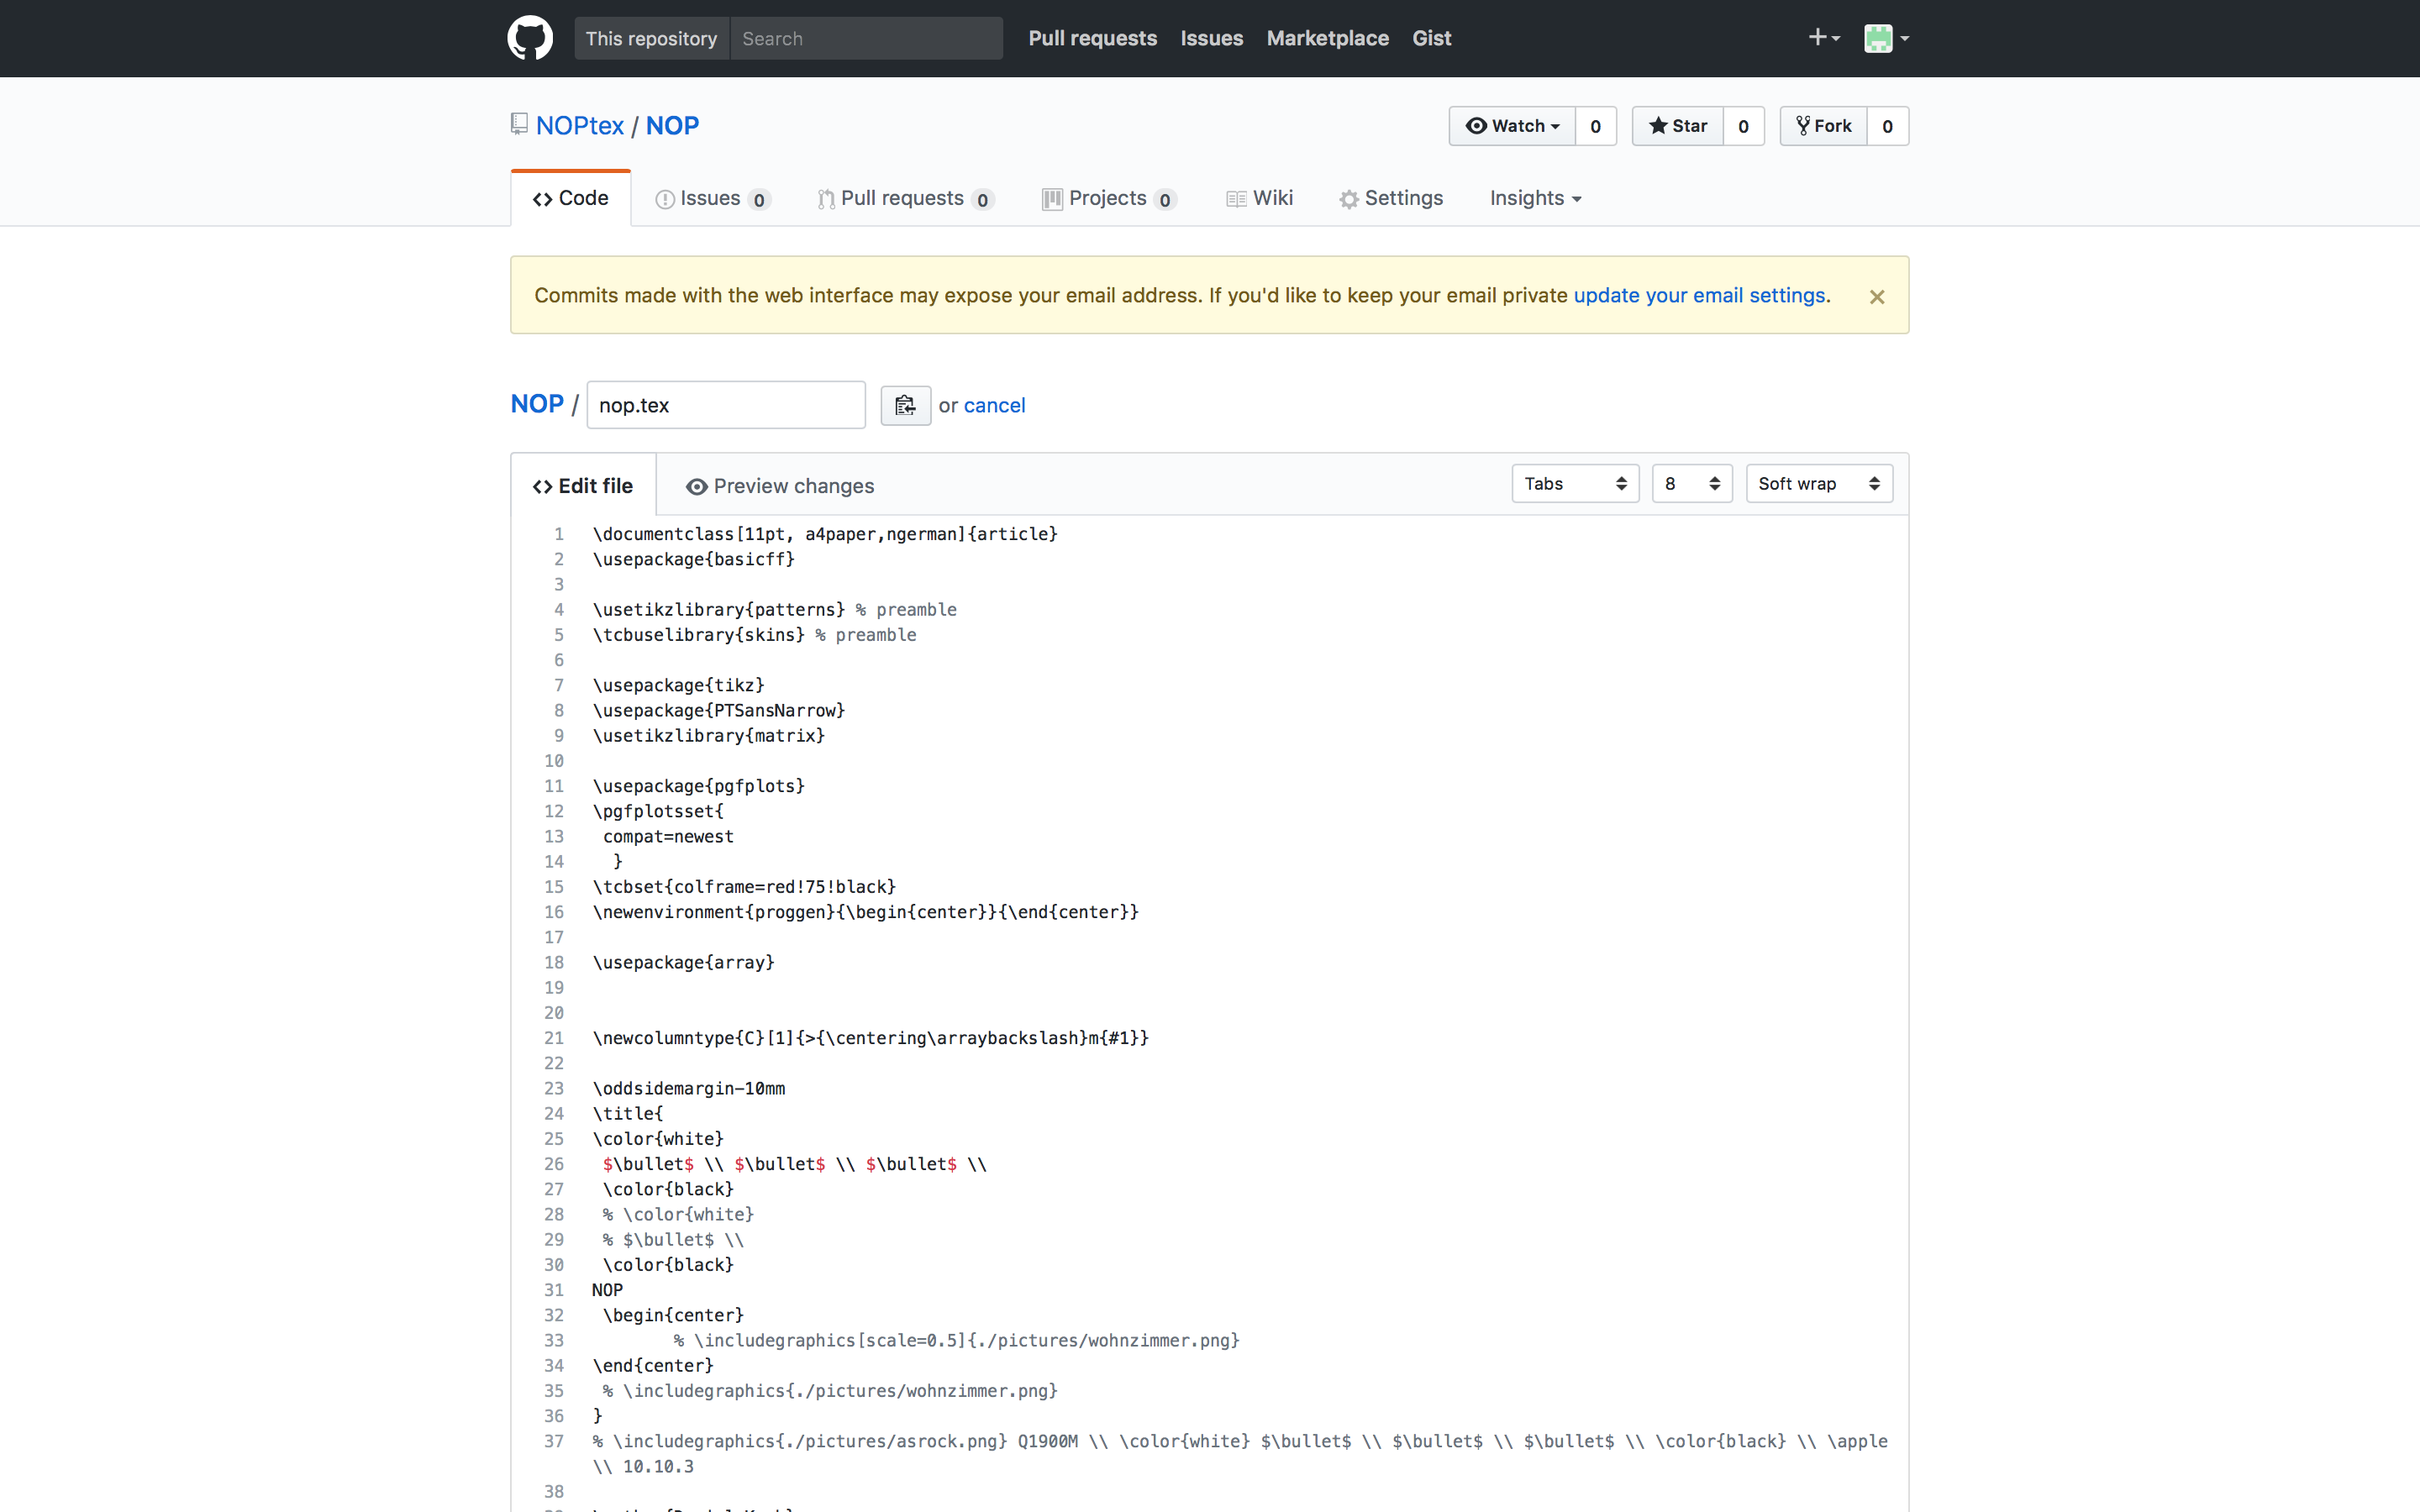
\includegraphics[width=1.0\textwidth]{./bilder/22edit.png}
% \end{framed}
%
% \end{minipage}}
% \hfill
% \adjustbox{valign=t}{\begin{minipage}[t]{0.45\textwidth}
% \vspace{0pt}
% \huge
% Die Anzeige ändert sich geringfüging.
% % \caption{Kapazität}
% \end{minipage}}
% \end{figure}
%
% \clearpage % GleitObjekte anzeigen



\newpage

\textbf{Wie gehts weiter / Nächste Schritte :}
\begin{itemize}
  \item Macports sauber auf macOS El Capitan installieren
  \item Texlive sauber installieren
  \item Rechte ordentlich setzen
\end{itemize}

\textbf{Dann baut es hoffentlich}
%
%
% \begin{figure}[]
%   \subsubsection{Github Repo mit Travis CI verbinden}
% \adjustbox{valign=t}{\begin{minipage}[t]{0.50\textwidth}
% \begin{framed}
%   \includegraphics[width=1.0\textwidth]{./bilder/1gitRepoSettings.png}
% \end{framed}
%
% \end{minipage}}
% % \hfill
% \adjustbox{valign=t}{\begin{minipage}[t]{0.5\textwidth}
% \vspace{0pt}
% \huge
% Im Repo klickt man auf Settings
% % \caption{Kapazität}
% \end{minipage}}
% % \end{figure}
% % \vspace{0.5cm} % ----------------------------------- vspace
% % \begin{figure}[ht]
% \adjustbox{valign=t}{\begin{minipage}[t]{0.40\textwidth}
% % \vspace{0.5cm}
% \begin{framed}
%   \includegraphics[width=1.0\textwidth]{./bilder/2integrationServices.png}
% \end{framed}
%
% \end{minipage}}
% \hfill
% \adjustbox{valign=t}{\begin{minipage}[t]{0.43\textwidth}
% \vspace{0pt}
% \huge
% Danach
% % \caption{Kapazität}
% \end{minipage}}
% \end{figure}
%
% \clearpage % GleitObjekte anzeigen
% \newpage
% \begin{table}
%   \caption{title}
% \end{table}
% Test


% \begin{center}
%  % \includegraphics[scale=0.5]{./pictures/wohnzimmer.png}
% \end{center}
% \begin{figure}
%     \subfigure[Bezeichnung der linken Grafik]{\includegraphics[width=0.49\textwidth]{./bilder/1gitRepoSettings.png}}
%     \subfigure[Bezeichnung der rechten Grafik]{\includegraphics[width=0.49\textwidth]{./bilder/2integrationServices.png}}
% \caption{Titel unterm gesamten Bild}
% \end{figure}


% \begin{figure}
%     \subfigure[Bezeichnung der linken Grafik]{\includegraphics[width=0.49\textwidth]{./bilder/1gitRepoSettings.png}}
%     \subfigure[Bezeichnung der rechten Grafik]{Test tesxt}
% \caption{Titel unterm gesamten Bild}
% \end{figure}










% \newpage
%
% \newpage
% bla
% \newpage
% bla
% \newpage
%
% \begin{figure}[ht]
% \adjustbox{valign=t}{\begin{minipage}[t]{0.66\textwidth}
% \includegraphics[width=1.0\textwidth]{./bilder/1gitRepoSettings.png}
% \end{minipage}}
% \hfill
% \adjustbox{valign=t}{\begin{minipage}[t]{150pt}
% \vspace{0pt}
% \huge
%
% % \caption{Kapazität}
% \end{minipage}}
% \end{figure}
%
% 3.1. Setup Github repo
% \newpage
% If you have forked this repo, then directly go to Settings option, otherwise, first create a new repository on Github and then, then go to Settings option of your repository.
% Click on Webhooks und Services and then Add service
% Select Travis CI
% Add your Travis CI username and Token
% Add service
% 3.2. Setup Travis CI
%
% Go to Travis CI
% Toggle on your repository
% 3.3. Install Travis Command-line Tool
%
% To configure Travis build to deploy generated PDF to Github releases, we have to get Github OAuth Token. To get it and securely embed it into .travis.yml file, we have to install Travis Command-line Tool
%
% gem install travis -v 1.7.5 --no-rdoc --no-ri
% travis setup releases
% Provide your Github username and password, to generate token and encrypt it on the go. This will also add it to your .travis.yml file.
  %  ARARA LUATEX

% 
\newpage

\section{Github + Travis CI - \ \  \"{} the pdflatex way \"{}}
\subsection{Was wird benötigt ?}
{\color{green}Kostenlose} Variante (nur public Repo's):
\begin{itemize}
  \item Ein Github - Account
  \item Ein Travis-CI (.org) Account
  \item Das Travis Command-line Tool
\end{itemize}
\vspace{0.5cm}
{\color{red}Kostenpflichtige} / Studenten Variante \\(Auch private Repo's / und sofortige build's):
\begin{itemize}
  \item Ein kostenpflichtiger Github - Account ( \$7/ Monat)
  \item Ein kostenpflichtiger Travis-CI (.com) Account ( \$69/ Monat)
  \item Alternativ ein Student Developer Pack von Github \\ siehe: https://education.github.com/pack
  \item Das Travis Command-line Tool
\end{itemize}


%
%   Seite 4
%
%   Github
%
\newpage
\subsection{Einrichtung}
\subsection{Github}
Als erstes benötigen wir einen Github Account inkl. Repo.
\begin{center}
  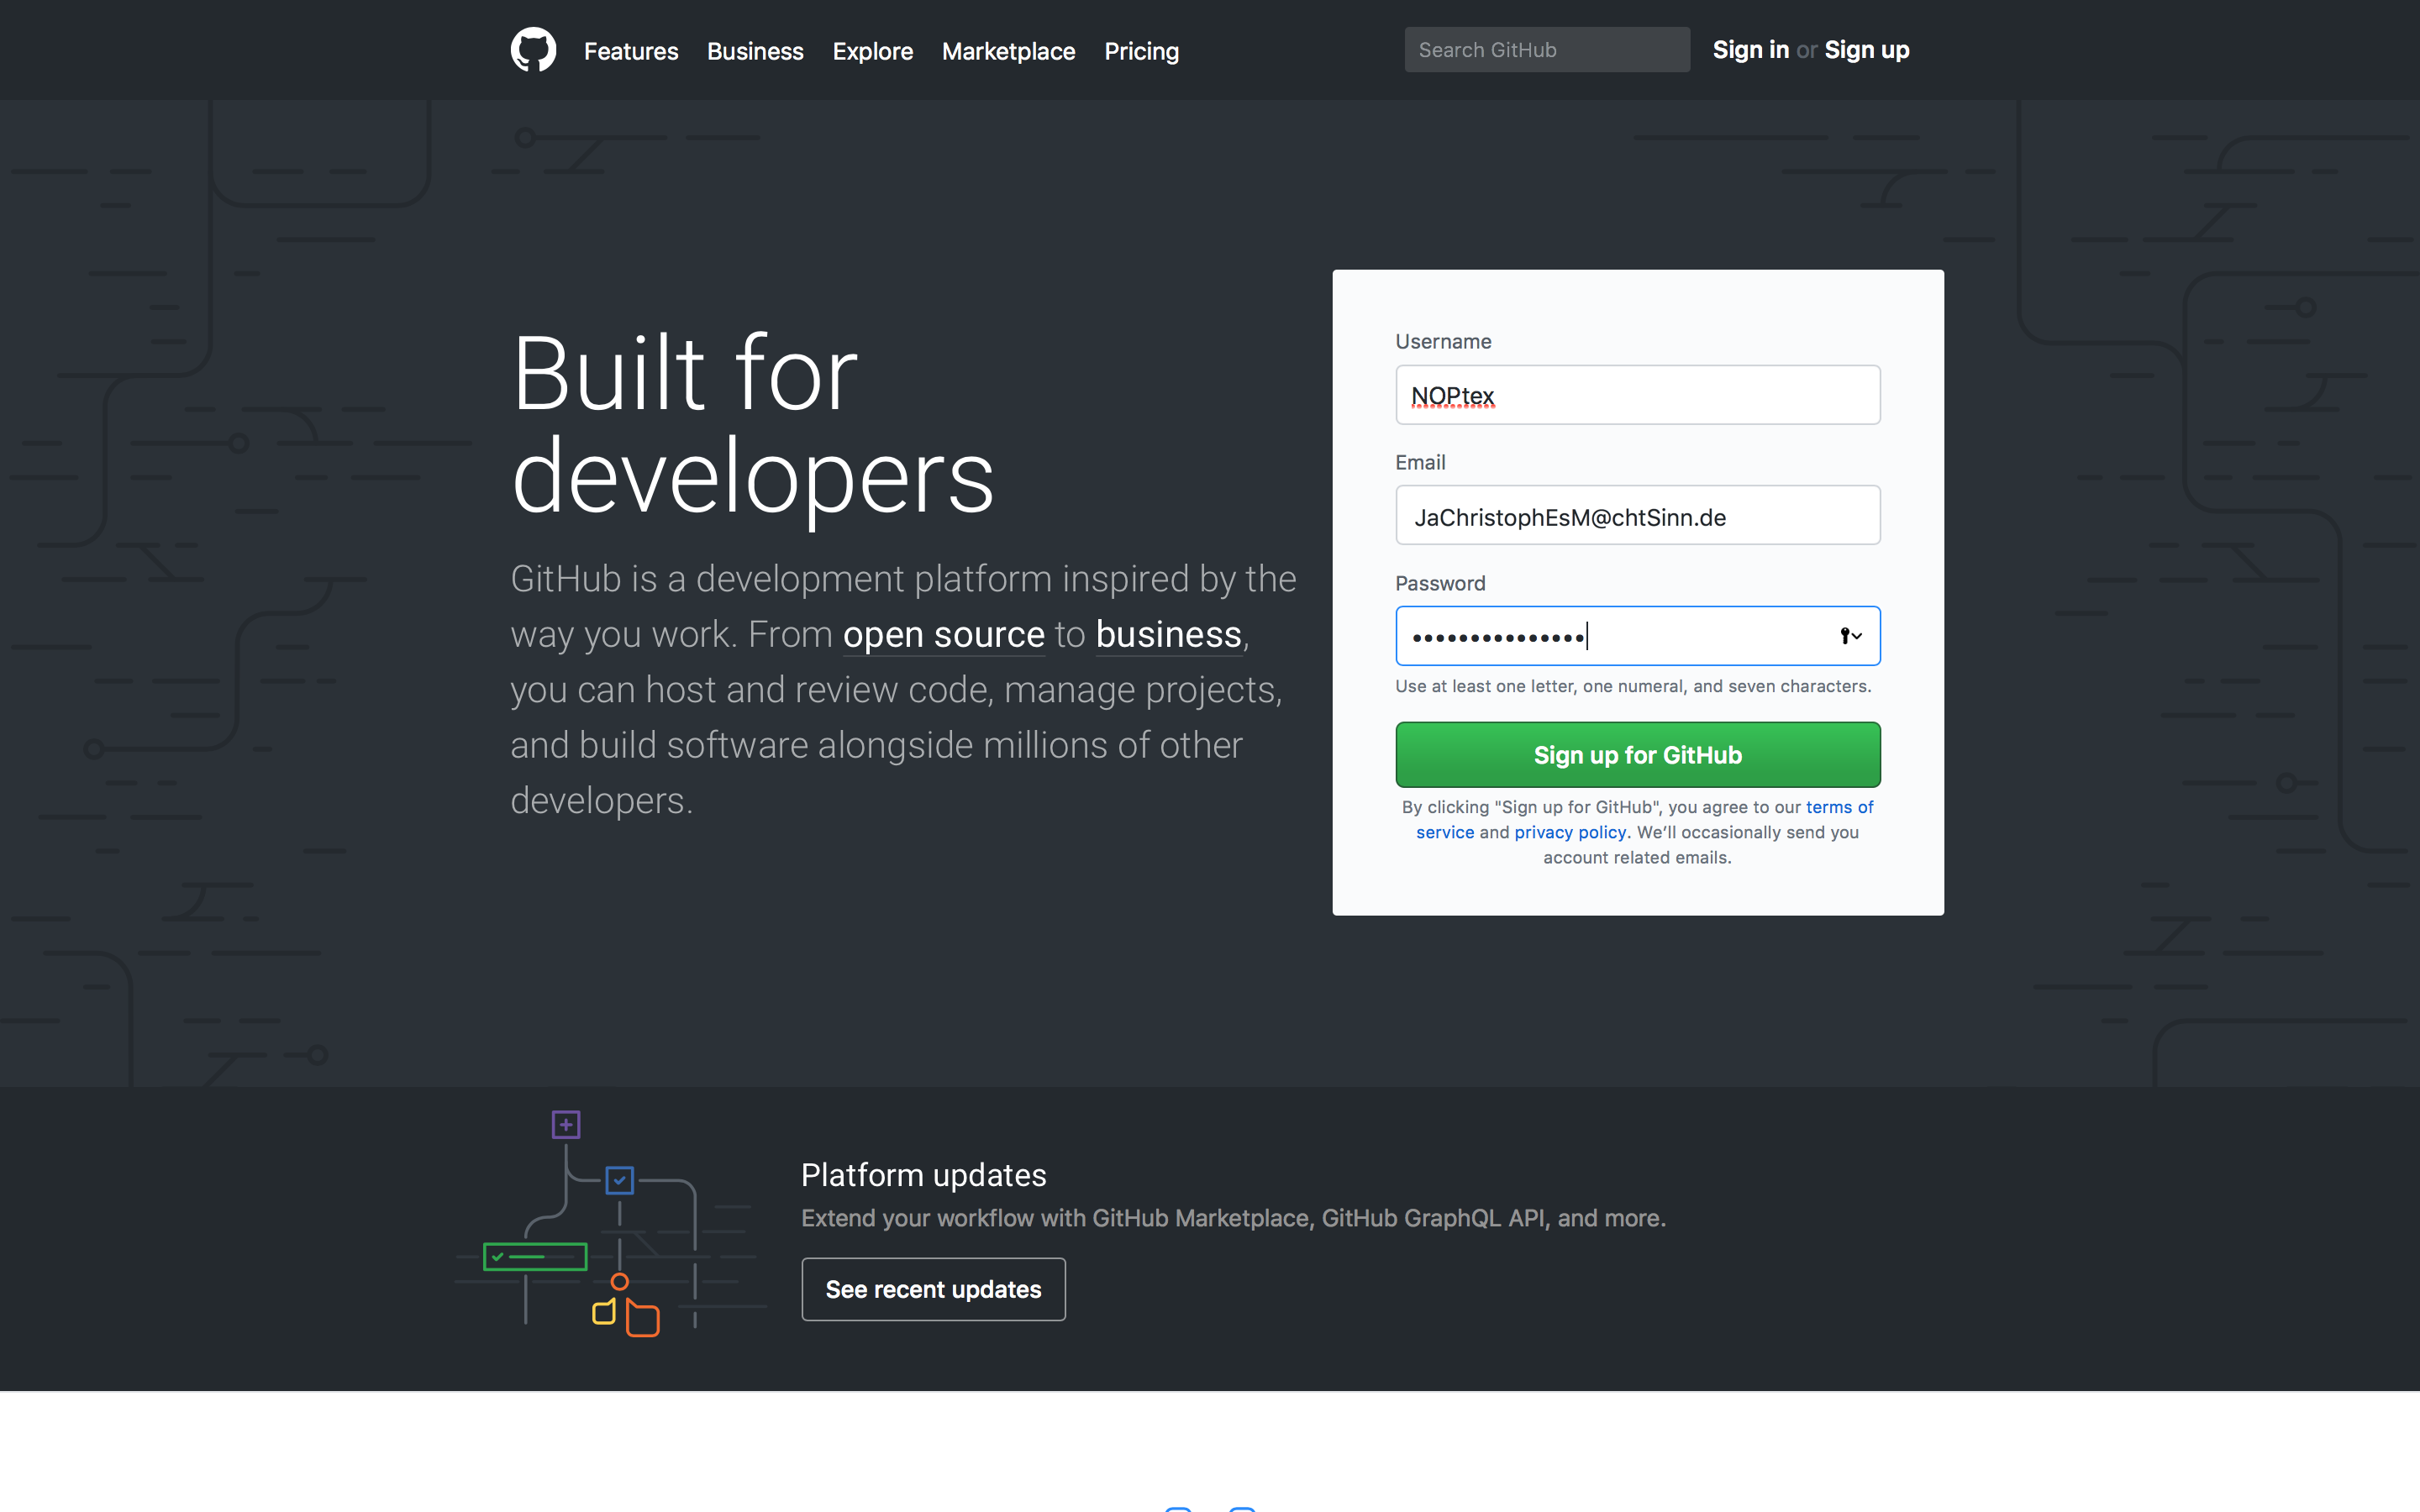
\includegraphics[trim = 300px 10px 300px 0px, clip,height=11cm]{./bilder/1Github.png}
\end{center}

% "l, b, r, t"
% \begin{figure}
% 	\centering
% \end{figure}\includegraphics[trim = 20px 10px 20px 30px, clip, width=\textwidth]{Beispiel.jpg}
% 	\caption{Hier steht der Beschriftungstext.}
% 	\label{fig:Beispiel}
% \end{figure}



\newpage
(Im Verlauf dieses Vortrages verwende ich:\\

https://github.com/NOPtex/NOP)\\


Dort befindet sich ein funktionierender Prototyp. \\
(Welcher aber noch ein paar zusätzlich Dateien beinhaltet.) \\

Prinzipiell reicht eine \TeX -Datei und die .travis.yml.

\begin{center}
  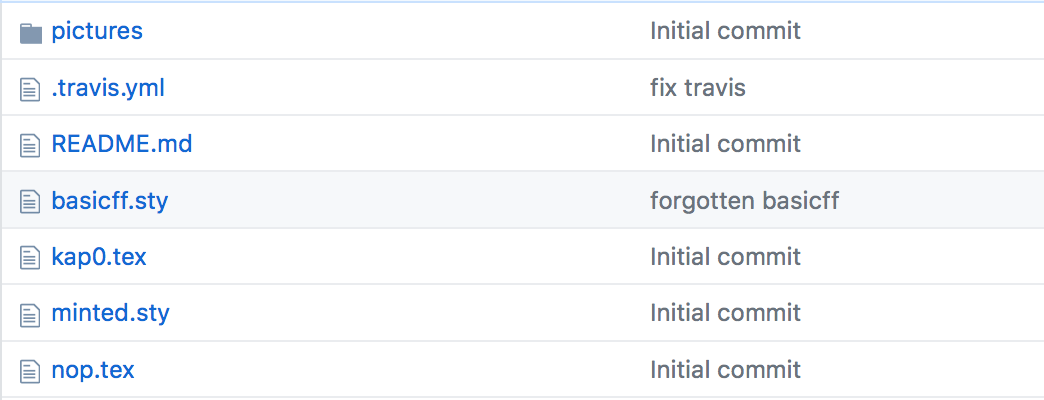
\includegraphics[width=0.8\textwidth]{./bilder/2Boilerplate.png}
\end{center}

%
%
% \vspace{0.5cm}
%
% \begin{center}
%   \includegraphics[width=1.0\textwidth]{./bilder/plainRepo.png}
% \end{center}

%
%   Seite 5
%
%   Github
% \cleardoublepage

\newpage % ============================================= Newpage ===================


\begin{figure}[ht]
  \subsection{Travis CI}
  \subsubsection{In Travis CI einloggen und mit Github verbinden}
\adjustbox{valign=t}{\begin{minipage}[t]{0.50\textwidth}
\begin{framed}
  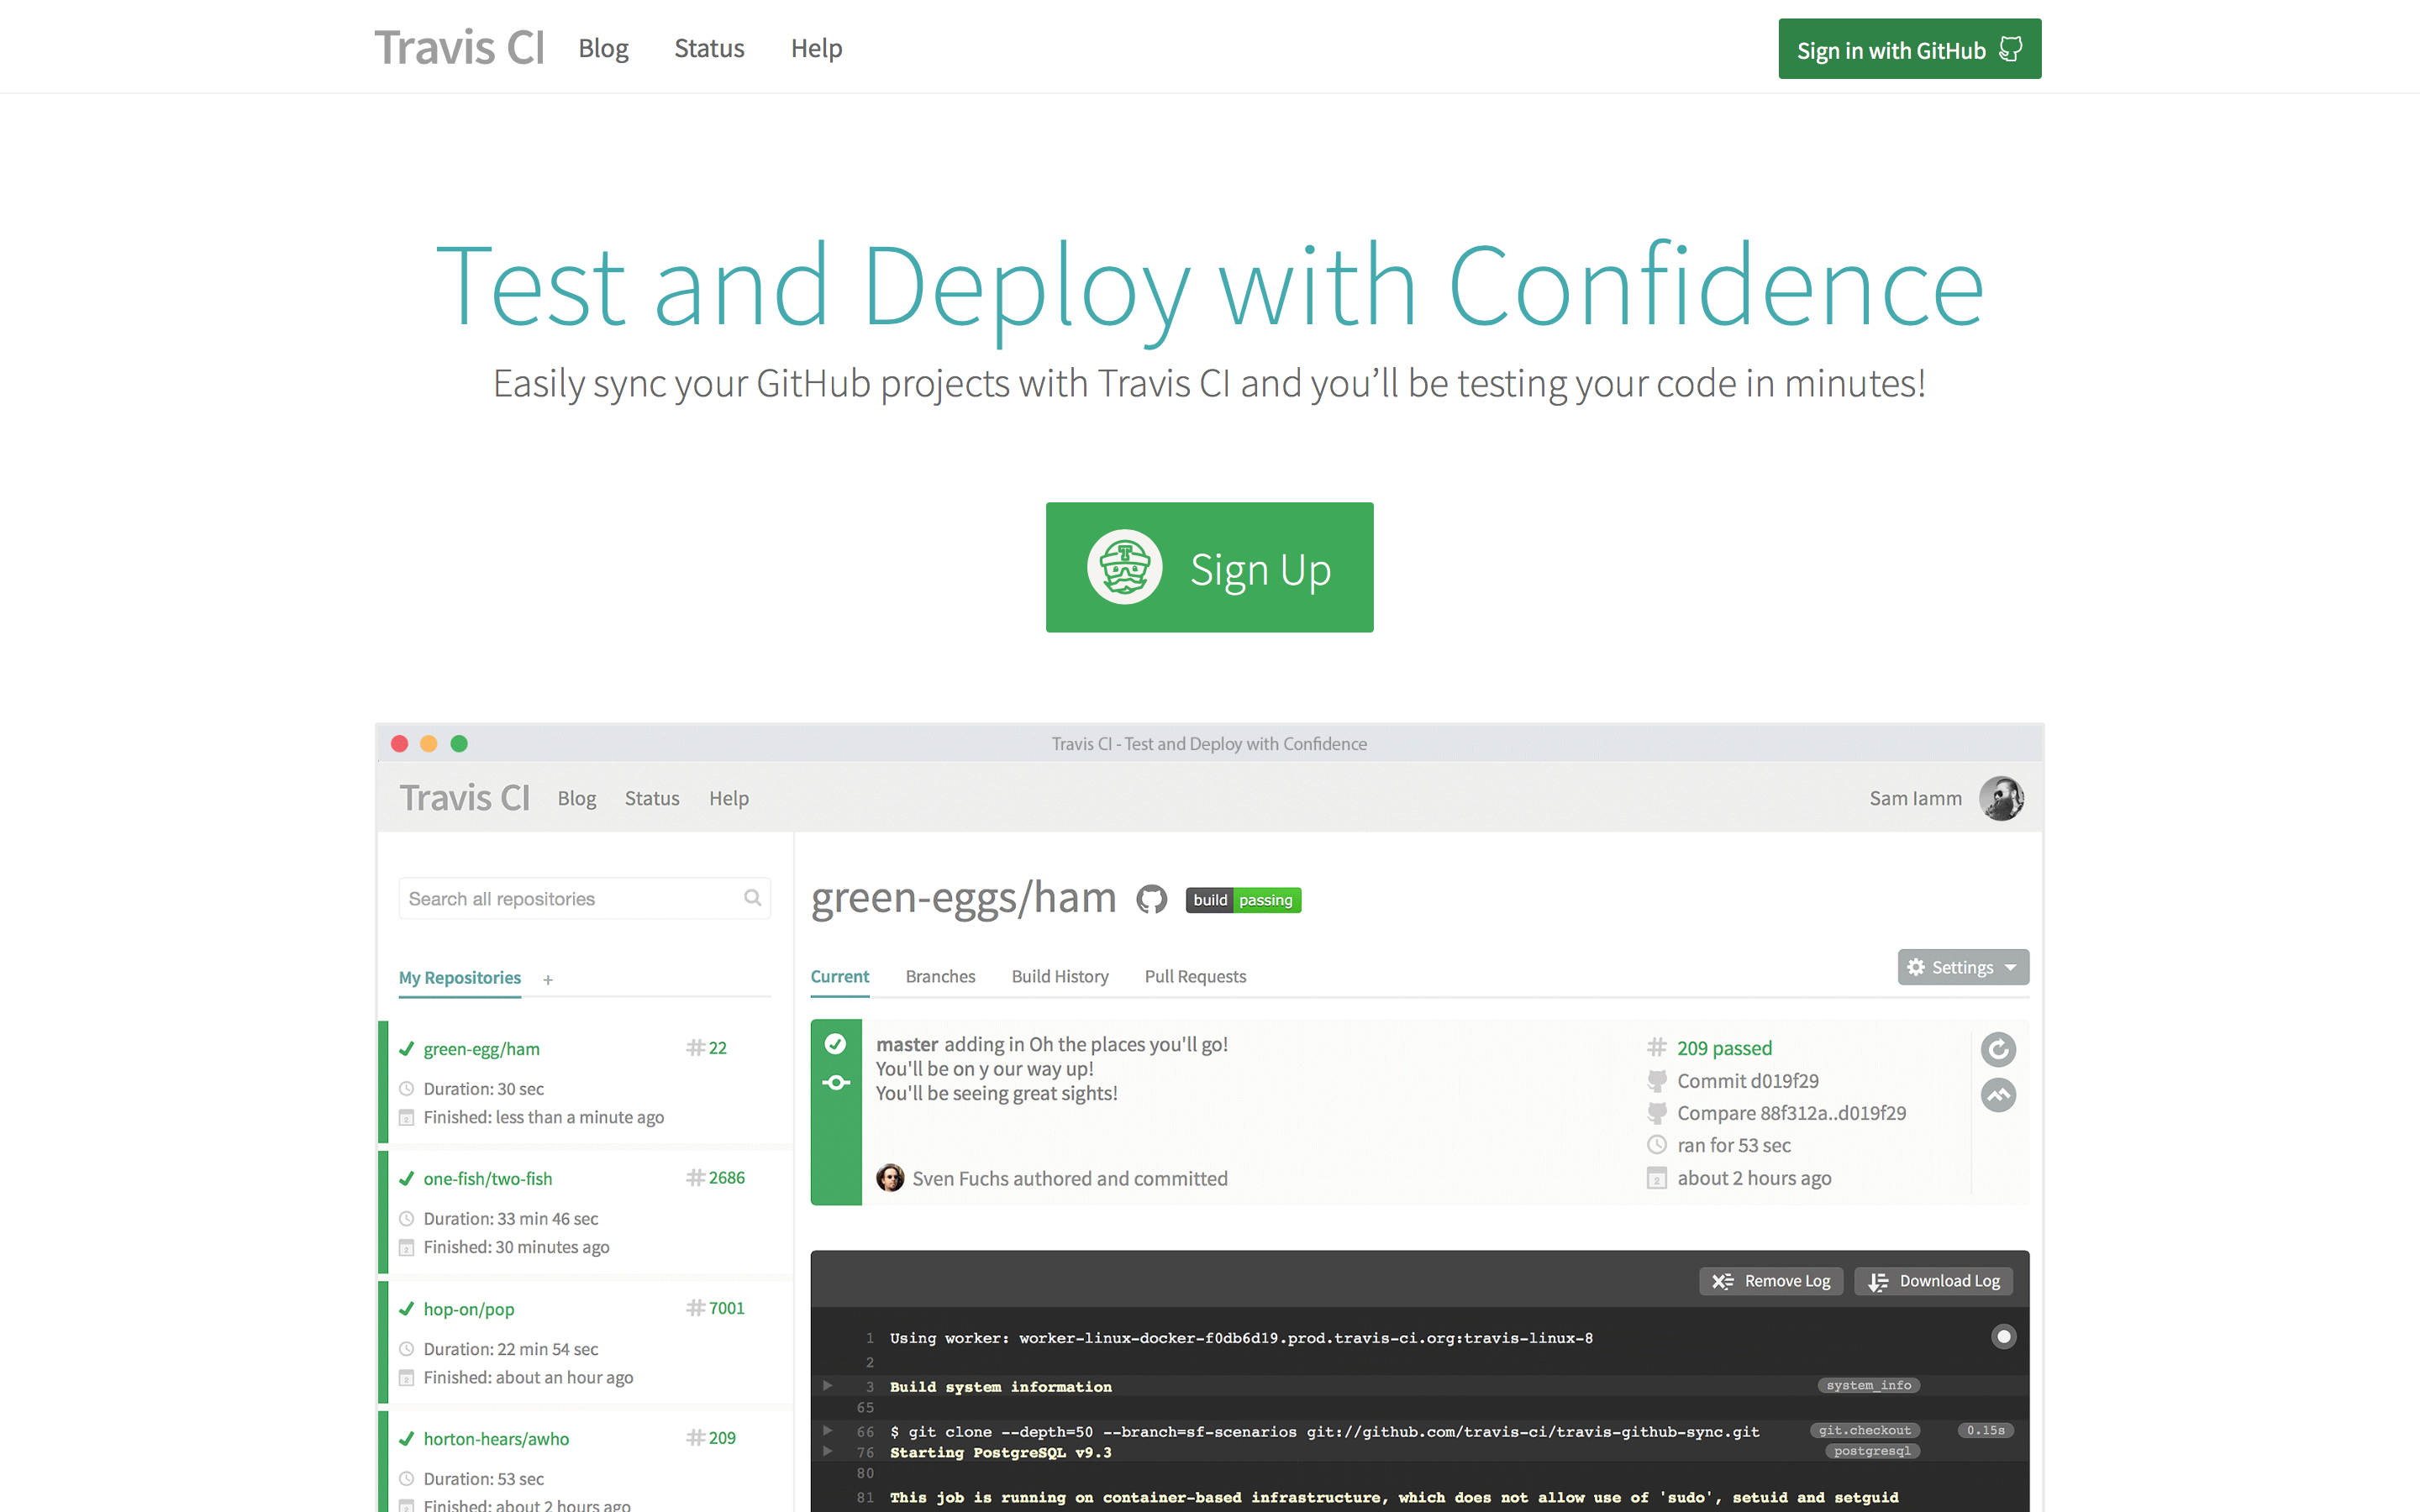
\includegraphics[width=1.0\textwidth]{./bilder/3travisSignUP.png}
\end{framed}

\end{minipage}}
% \hfill
\adjustbox{valign=t}{\begin{minipage}[t]{0.45\textwidth}
\vspace{0pt}
\huge
Da Travis nur mit Github \\funktioniert ist die Einrichtung recht \"{}trivial\"{}.
% \caption{Kapazität}
\end{minipage}}
% \end{figure}
% \vspace{0.5cm} % ----------------------------------- vspace
% \begin{figure}[ht]
\adjustbox{valign=t}{\begin{minipage}[t]{0.50\textwidth}
% \vspace{0.5cm}
\begin{framed}
  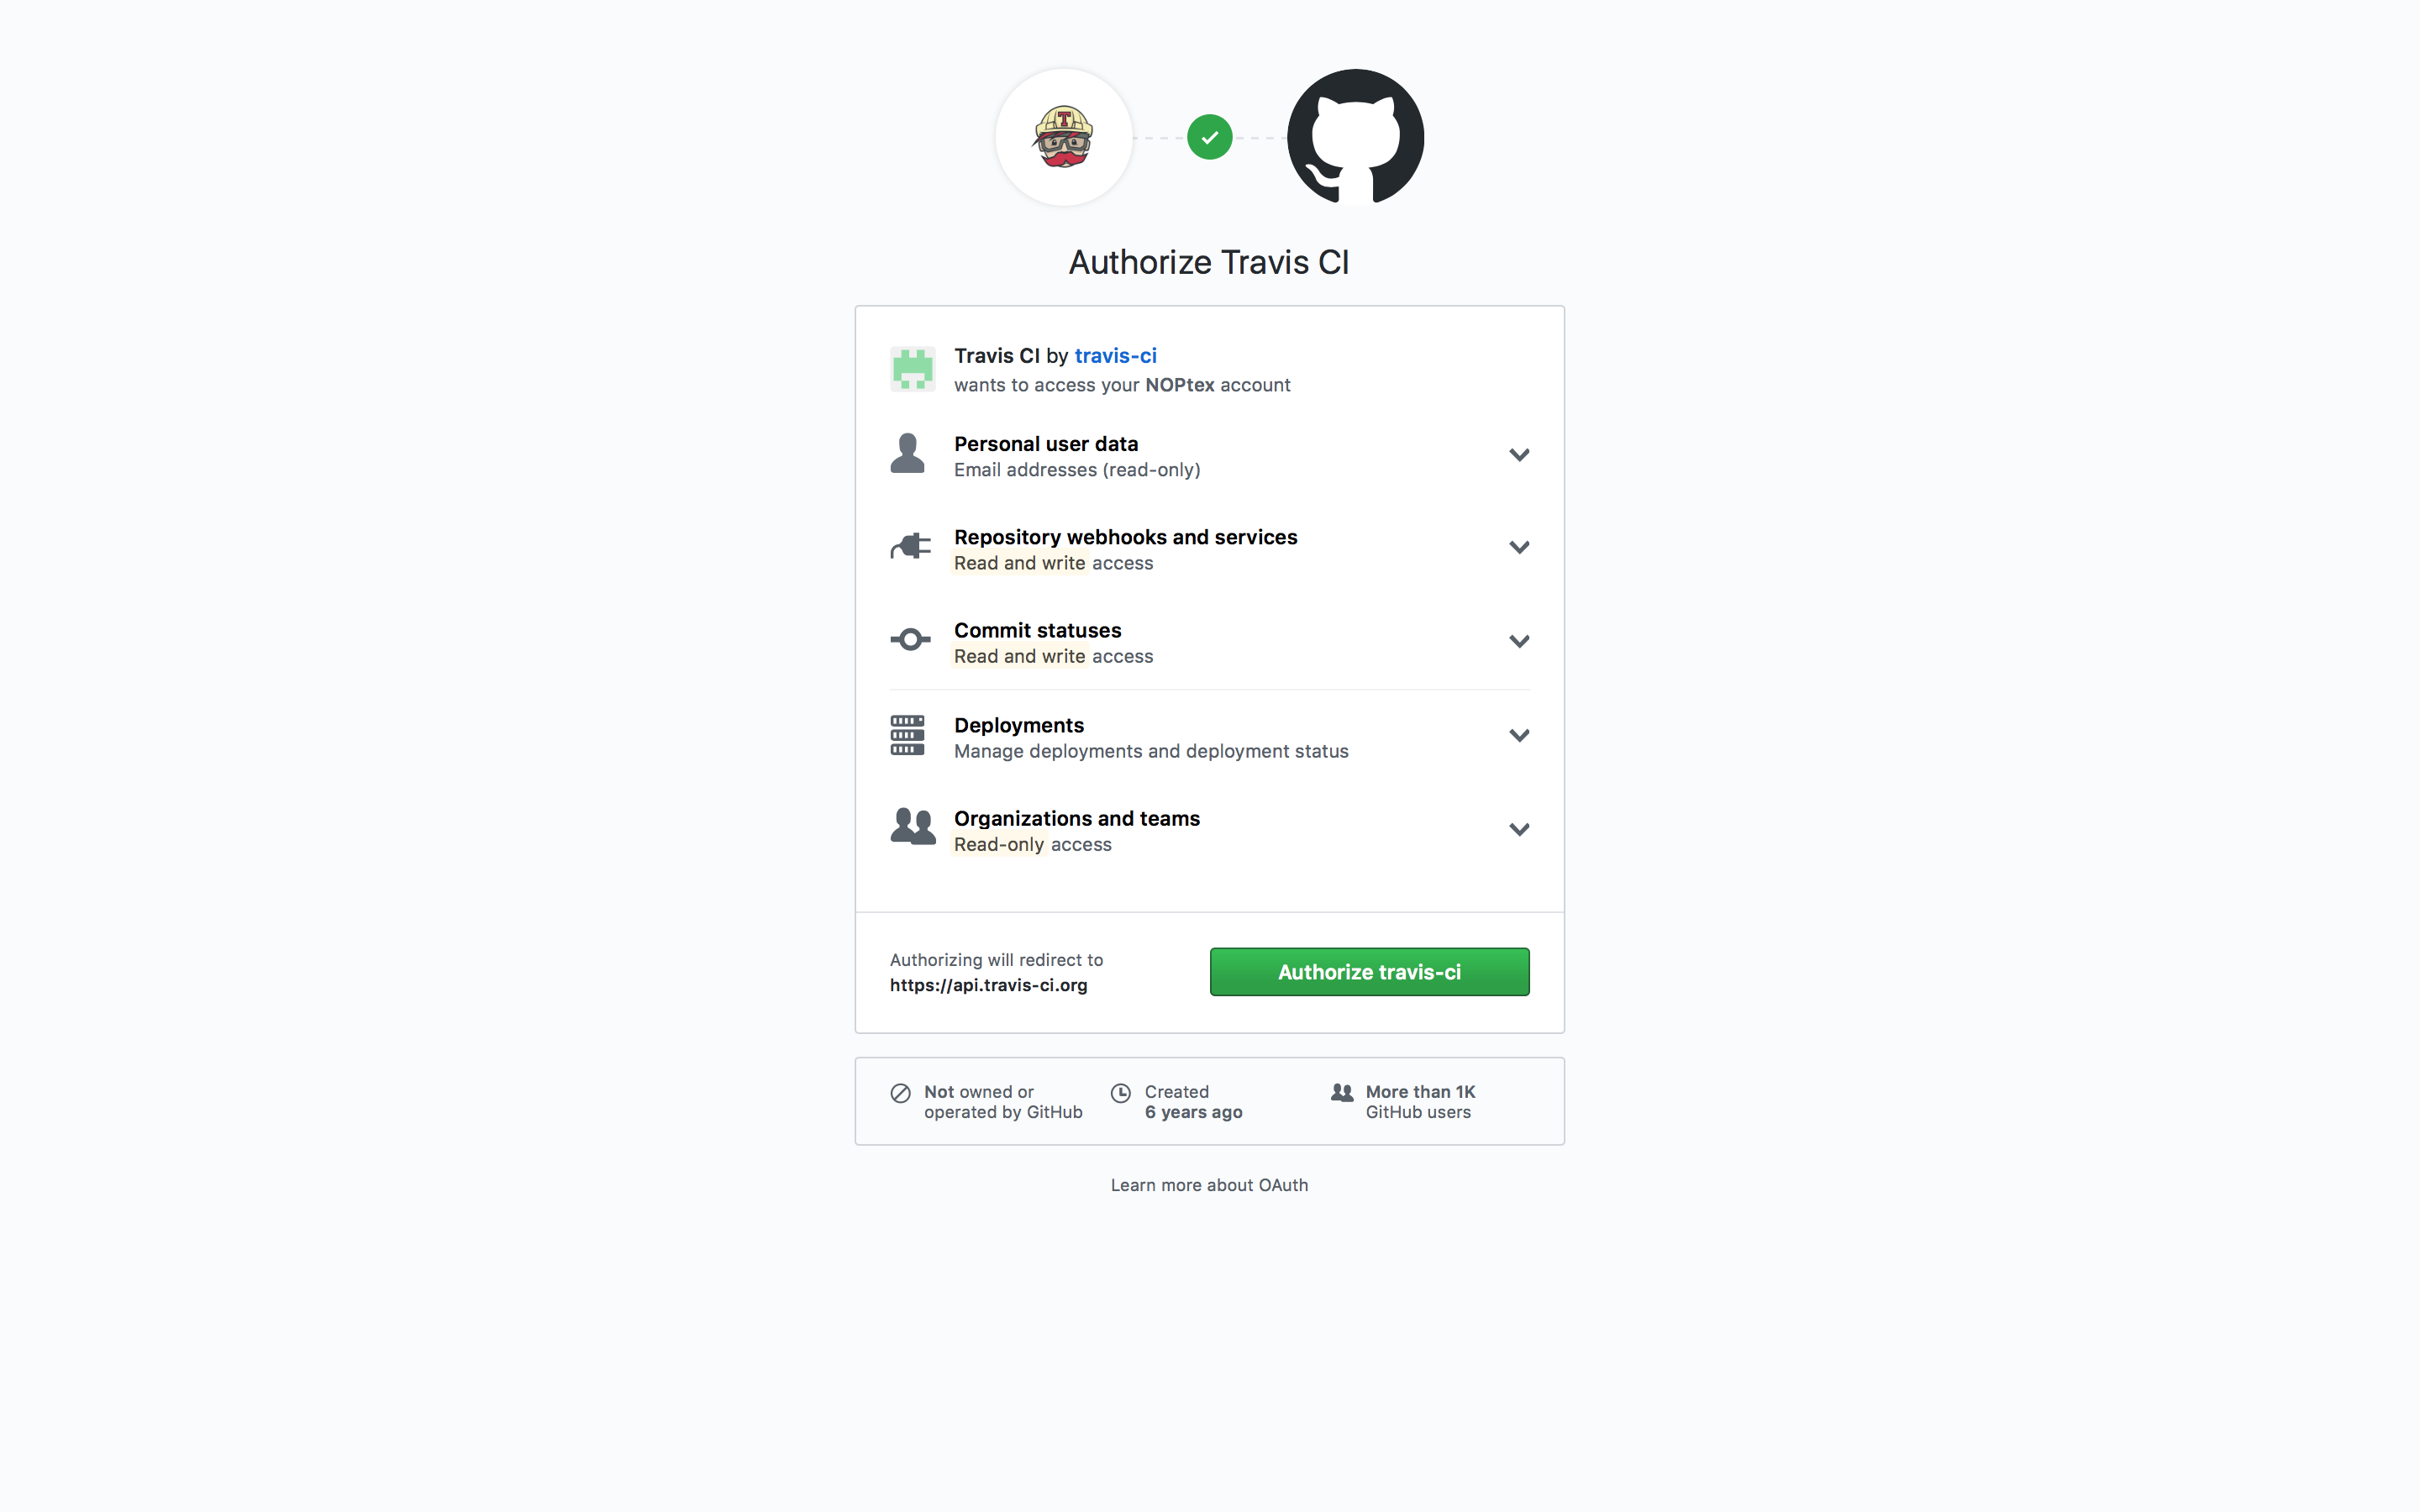
\includegraphics[width=1.0\textwidth]{./bilder/4TRAVISauthGITHUB.png}
\end{framed}

\end{minipage}}
\hfill
\adjustbox{valign=t}{\begin{minipage}[t]{0.45\textwidth}
\vspace{0pt}
\huge
Travis benötigt einige \\Berechtigungen welche man in diesem Schritt erteilt.
% \caption{Kapazität}
\end{minipage}}
\end{figure}

\clearpage % GleitObjekte anzeigen






\newpage % ============================================= Newpage ===================


\begin{figure}[ht]
  \subsubsection{Github - Repo aktivieren}
\adjustbox{valign=t}{\begin{minipage}[t]{0.50\textwidth}
\begin{framed}
  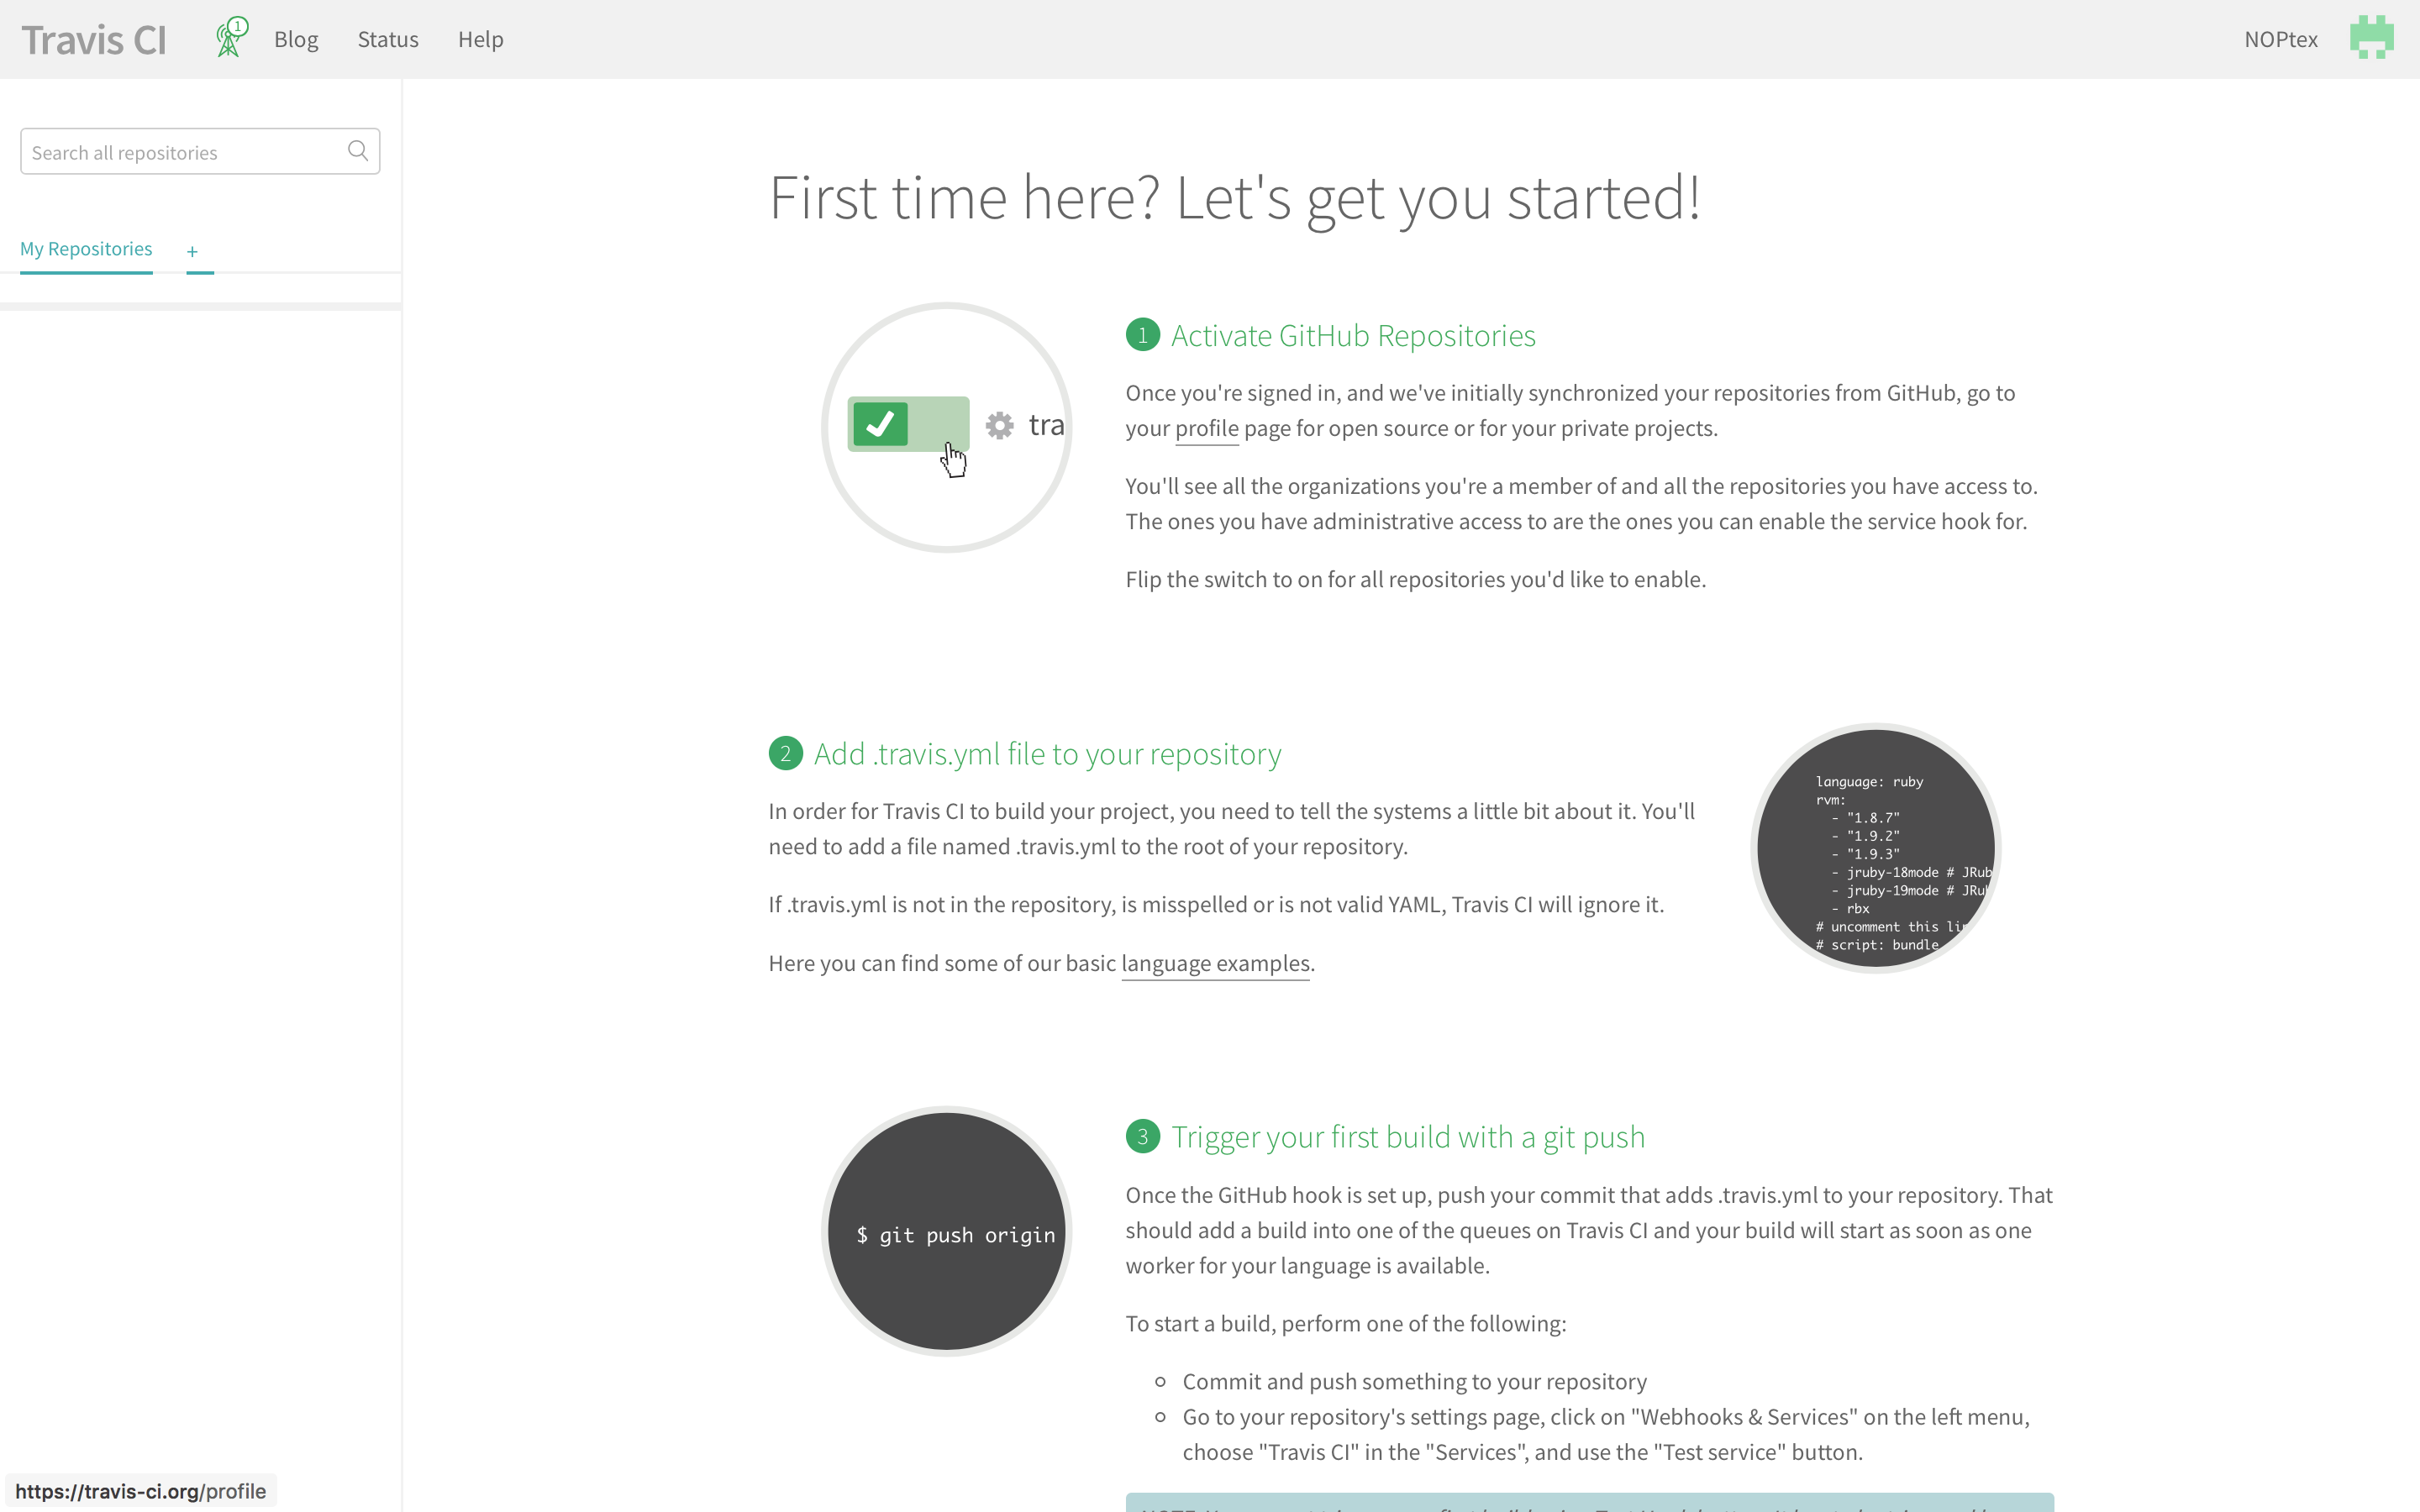
\includegraphics[width=1.0\textwidth]{./bilder/5TRAVISfirstSignIn.png}
\end{framed}

\end{minipage}}
% \hfill
\adjustbox{valign=t}{\begin{minipage}[t]{0.45\textwidth}
\vspace{0pt}
\huge
Da Travis nur mit Github funktioniert ist die Einrichtung recht einfach.
% \caption{Kapazität}
\end{minipage}}
% \end{figure}
% \vspace{0.5cm} % ----------------------------------- vspace
% \begin{figure}[ht]
\adjustbox{valign=t}{\begin{minipage}[t]{0.50\textwidth}
% \vspace{0.5cm}
\begin{framed}
  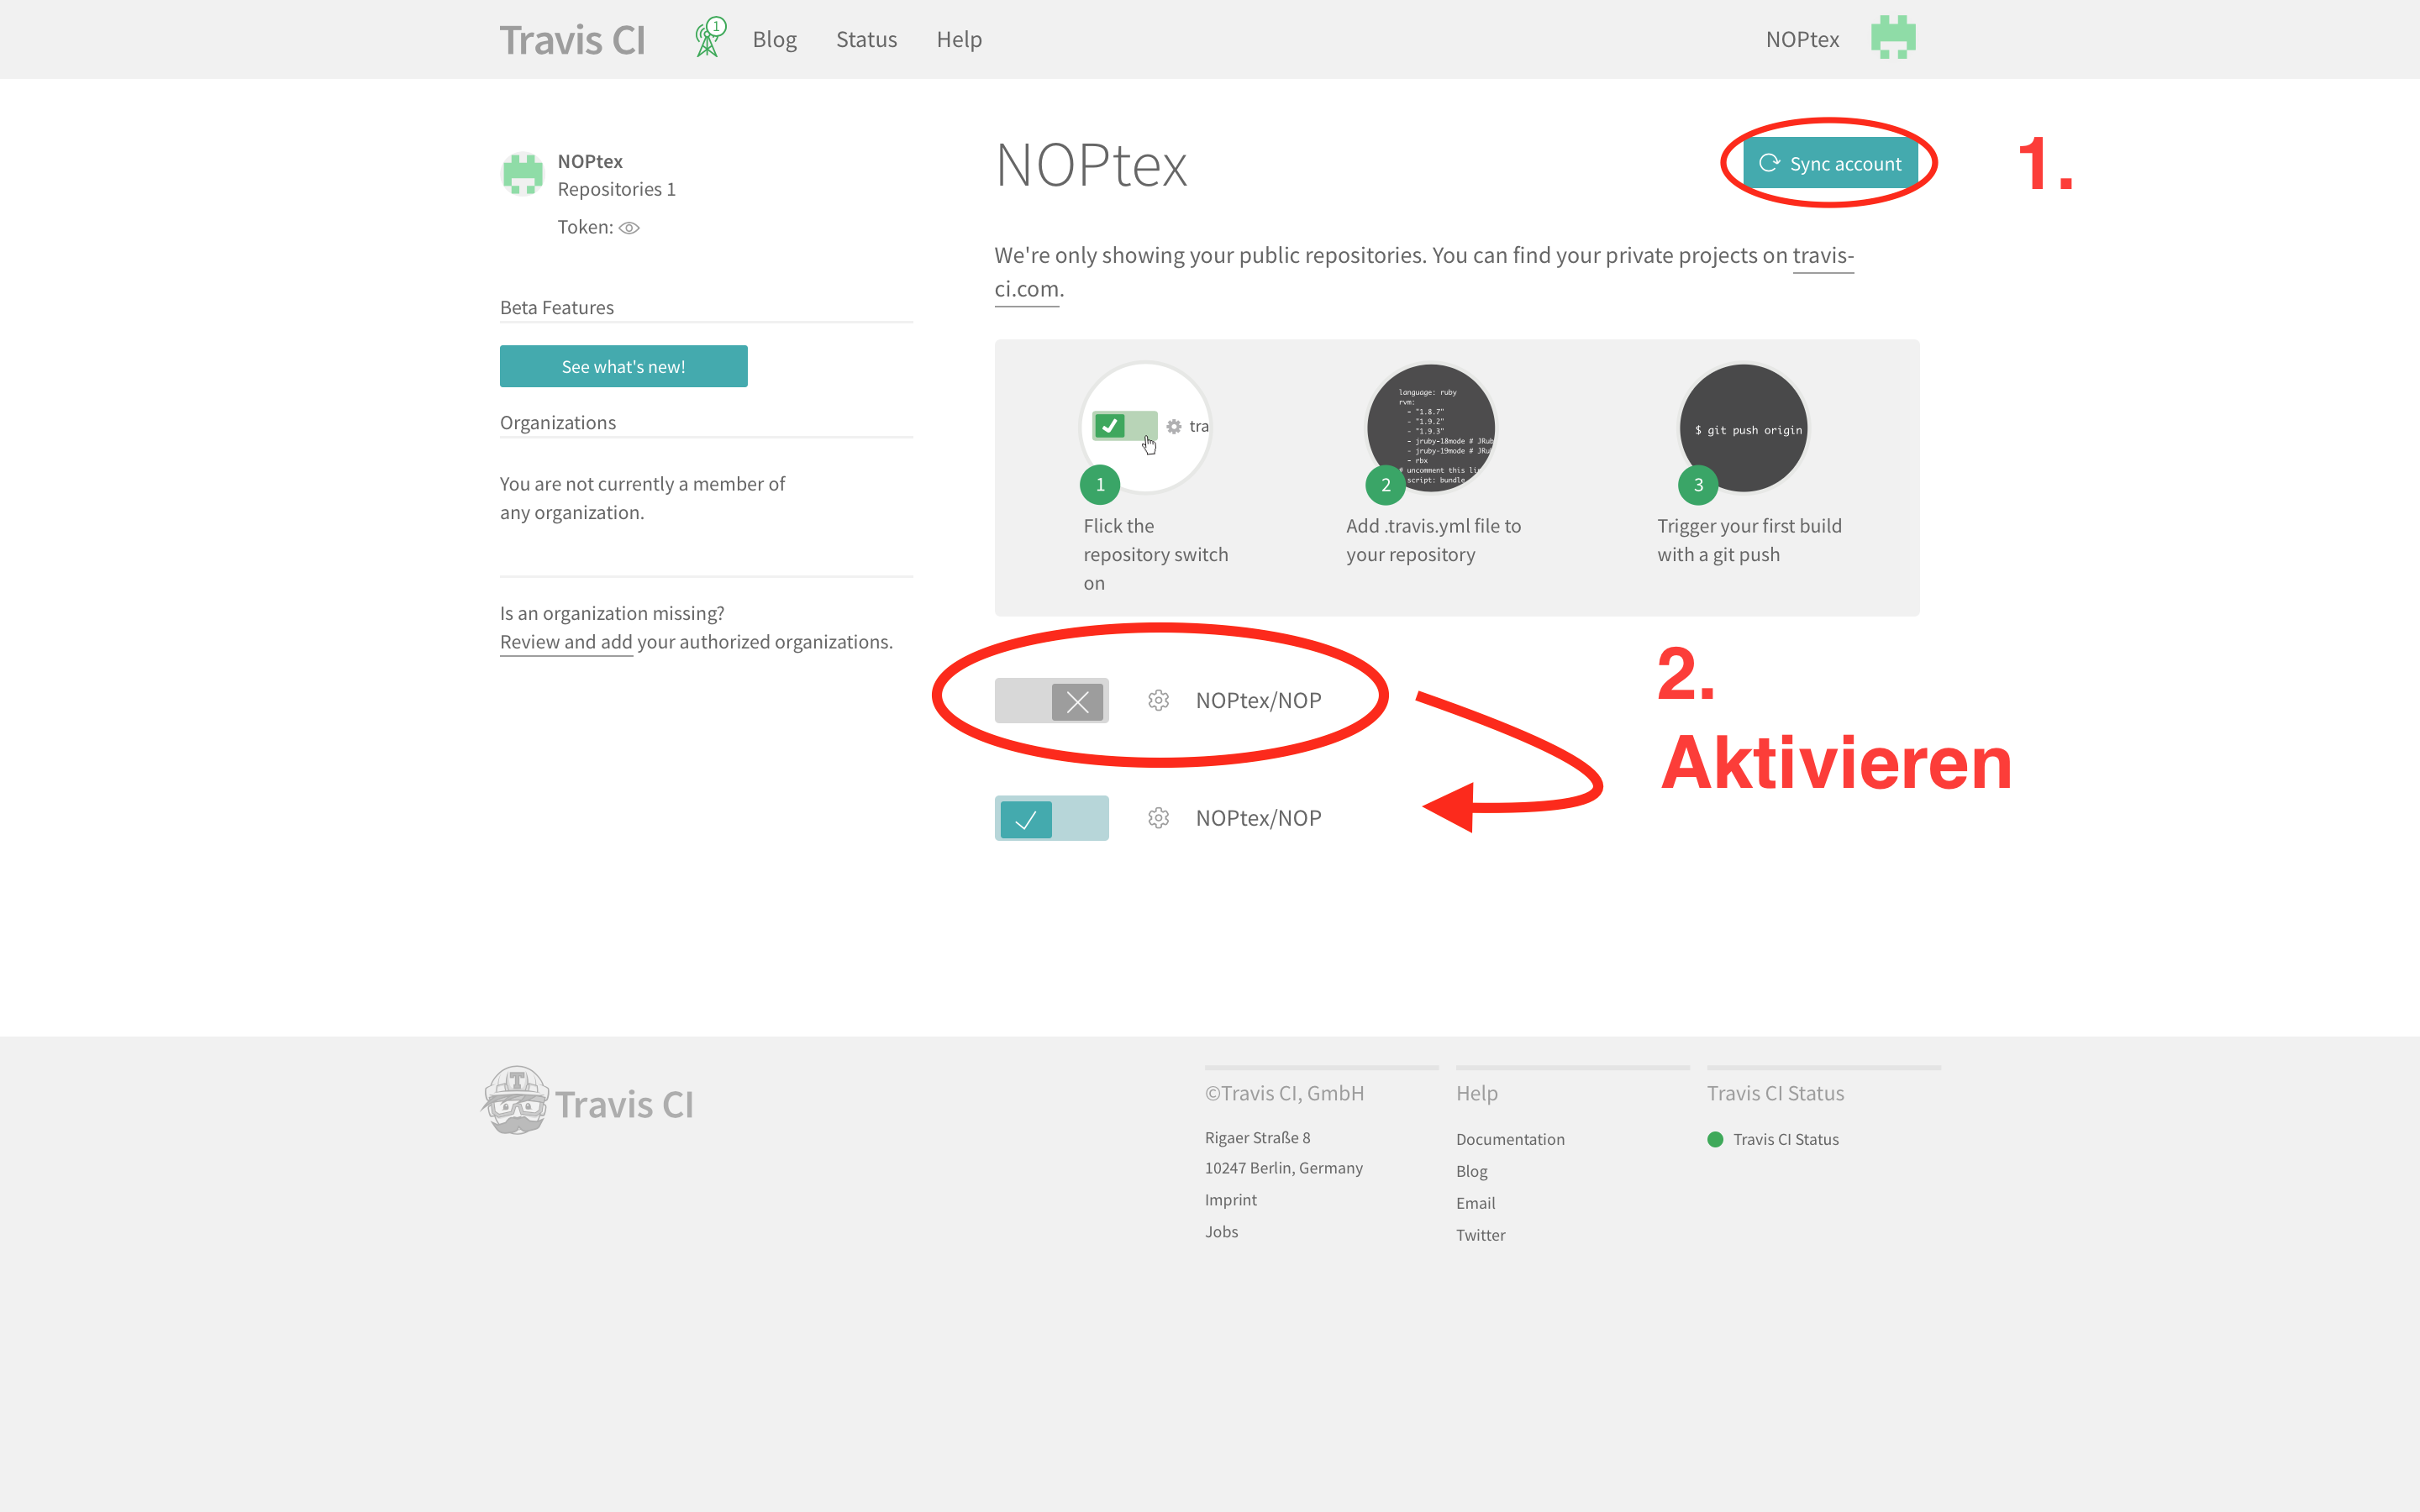
\includegraphics[width=1.0\textwidth]{./bilder/6TRAVISActivateREPO.png}
\end{framed}

\end{minipage}}
\hfill
\adjustbox{valign=t}{\begin{minipage}[t]{0.45\textwidth}
\vspace{0pt}
\huge
Travis benötigt einige Berechtigungen welche man im nächsten Schritt erteilt.
% \caption{Kapazität}
\end{minipage}}
\end{figure}

\clearpage % GleitObjekte anzeigen


\newpage % ============================================= Newpage ===================


\begin{figure}[ht]
  \subsubsection{Build-Einstellungen setzen}
\adjustbox{valign=t}{\begin{minipage}[t]{0.50\textwidth}
\begin{framed}
  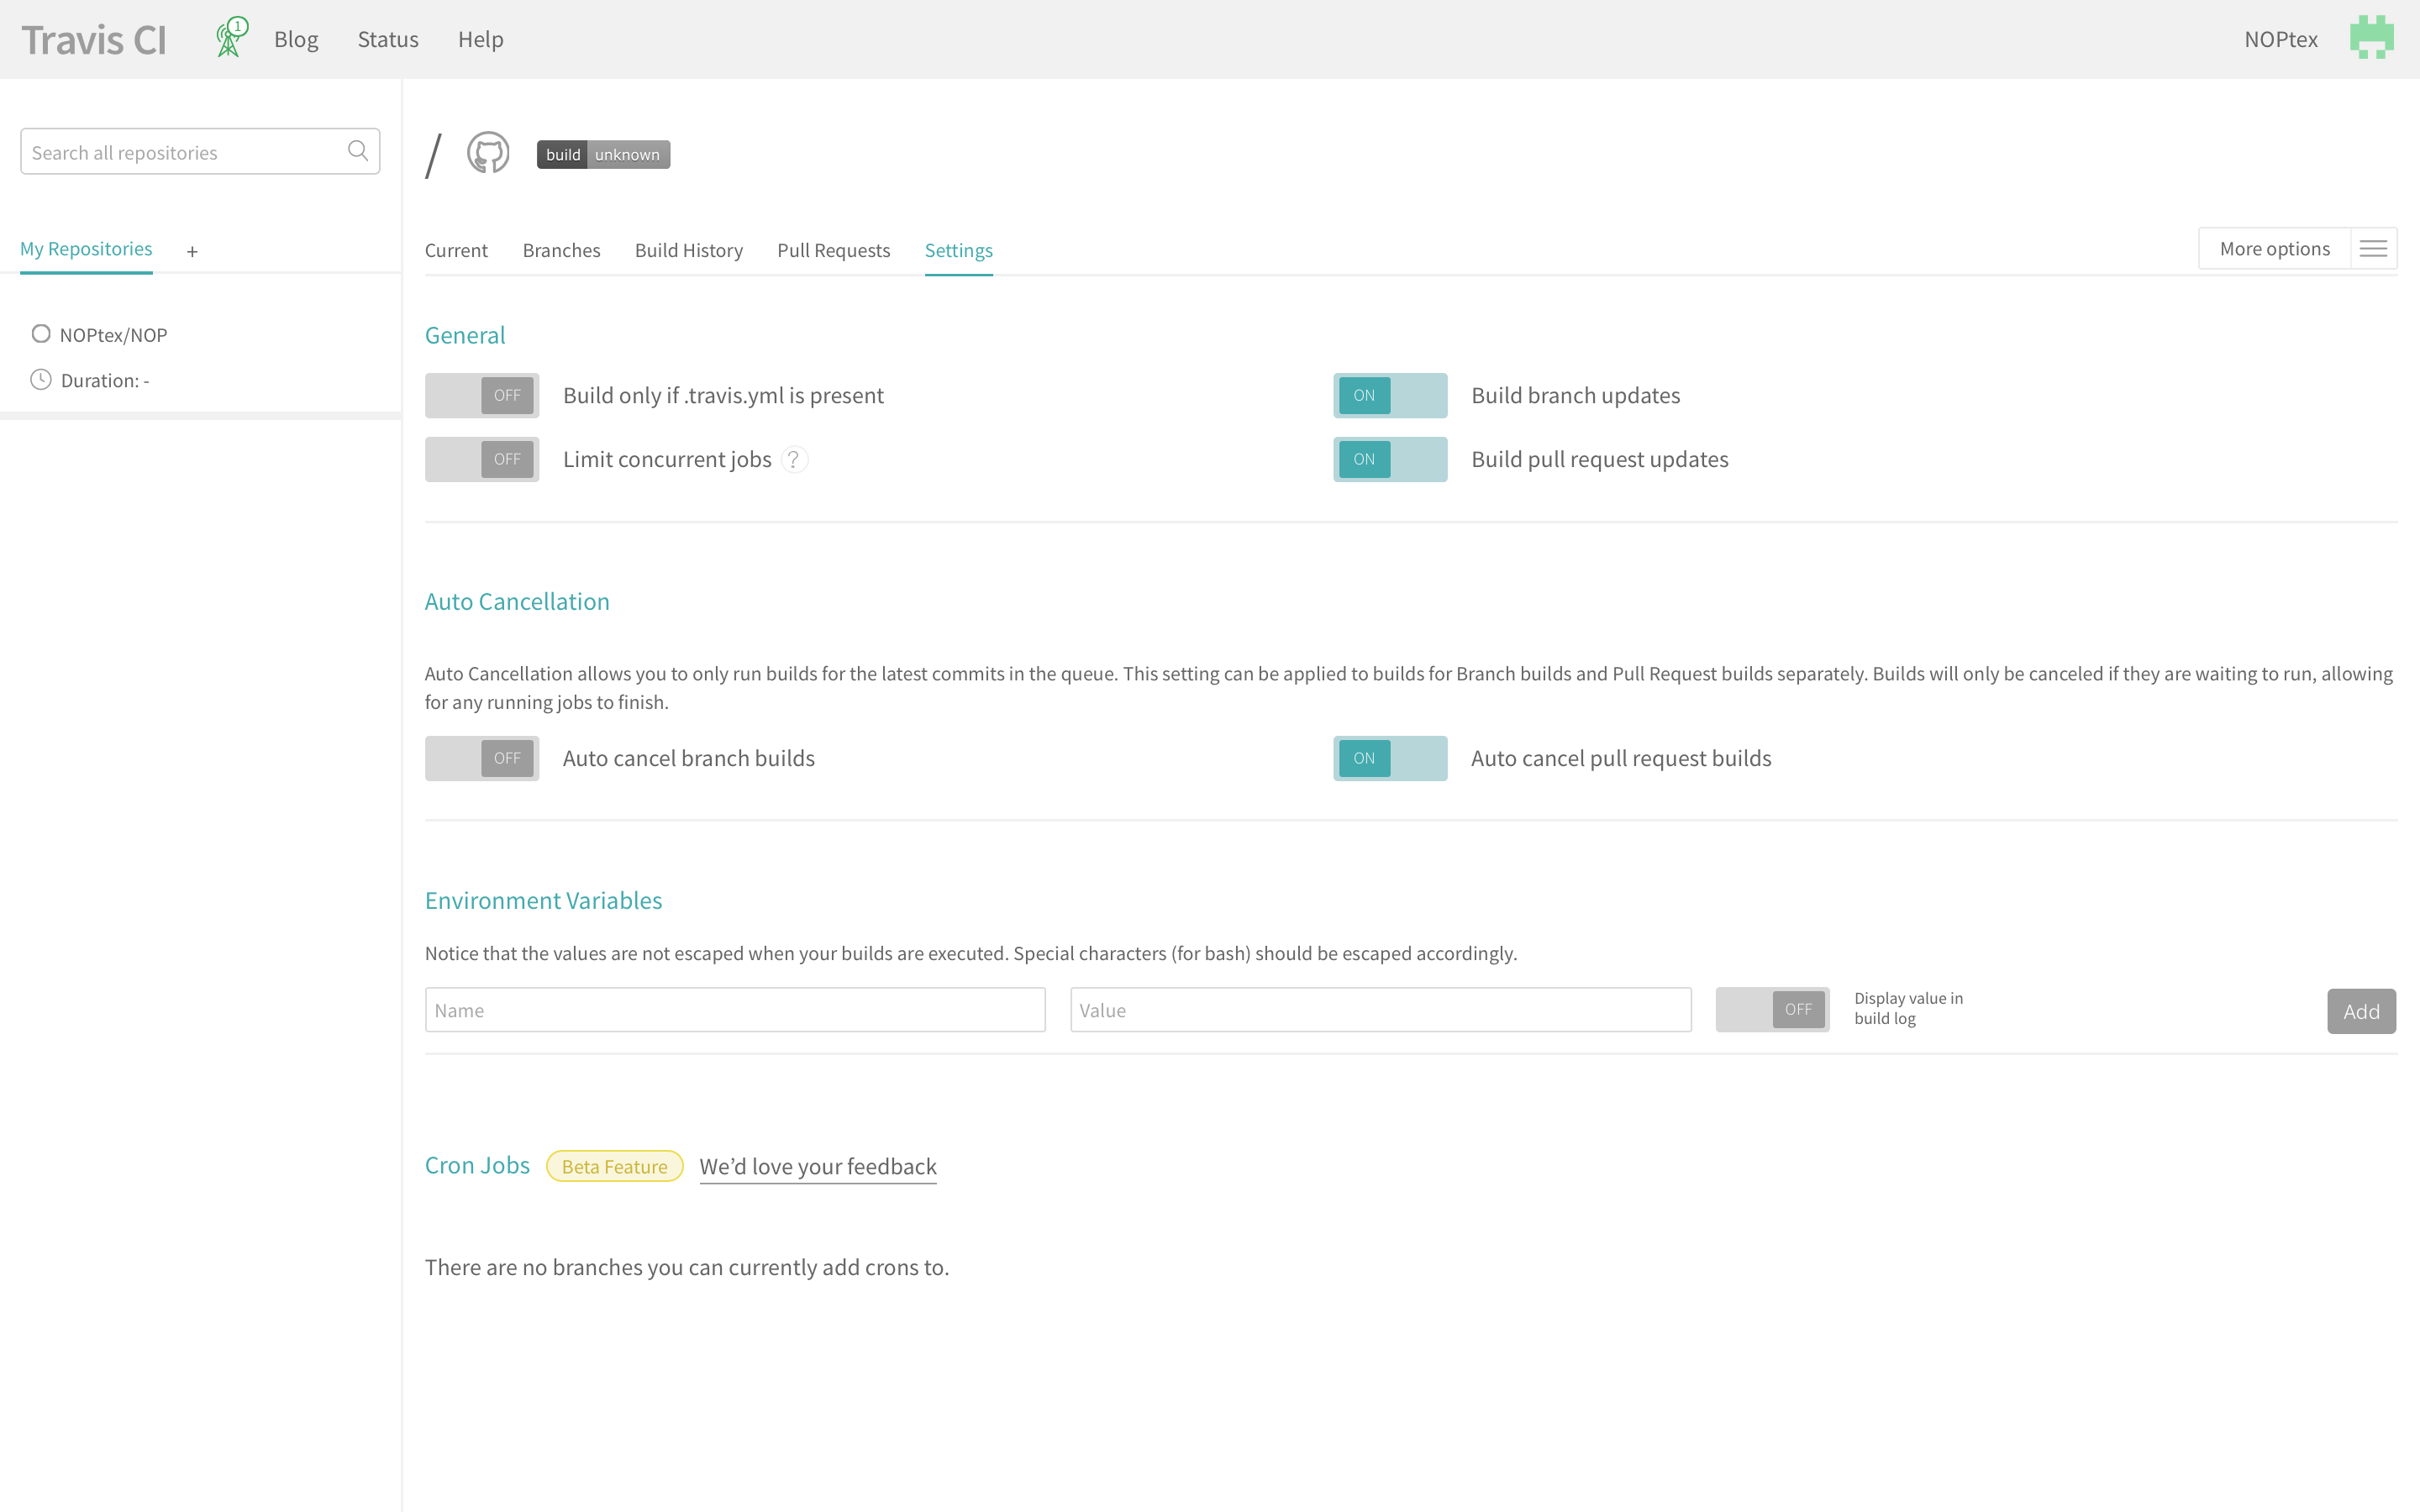
\includegraphics[width=1.0\textwidth]{./bilder/7TRAVISOptionsbase.png}
\end{framed}

\end{minipage}}
% \hfill
\adjustbox{valign=t}{\begin{minipage}[t]{0.45\textwidth}
\vspace{0pt}

\includegraphics[width=1.0\textwidth]{./bilder/7_1REPOsettings.png}
\huge
Über das Zahnrad kommt man zu den Einstellungen.
% \caption{Kapazität}
\end{minipage}}
% \end{figure}
% \vspace{0.5cm} % ----------------------------------- vspace
% \begin{figure}[ht]
\adjustbox{valign=t}{\begin{minipage}[t]{0.50\textwidth}
% \vspace{0.5cm}
\begin{framed}
  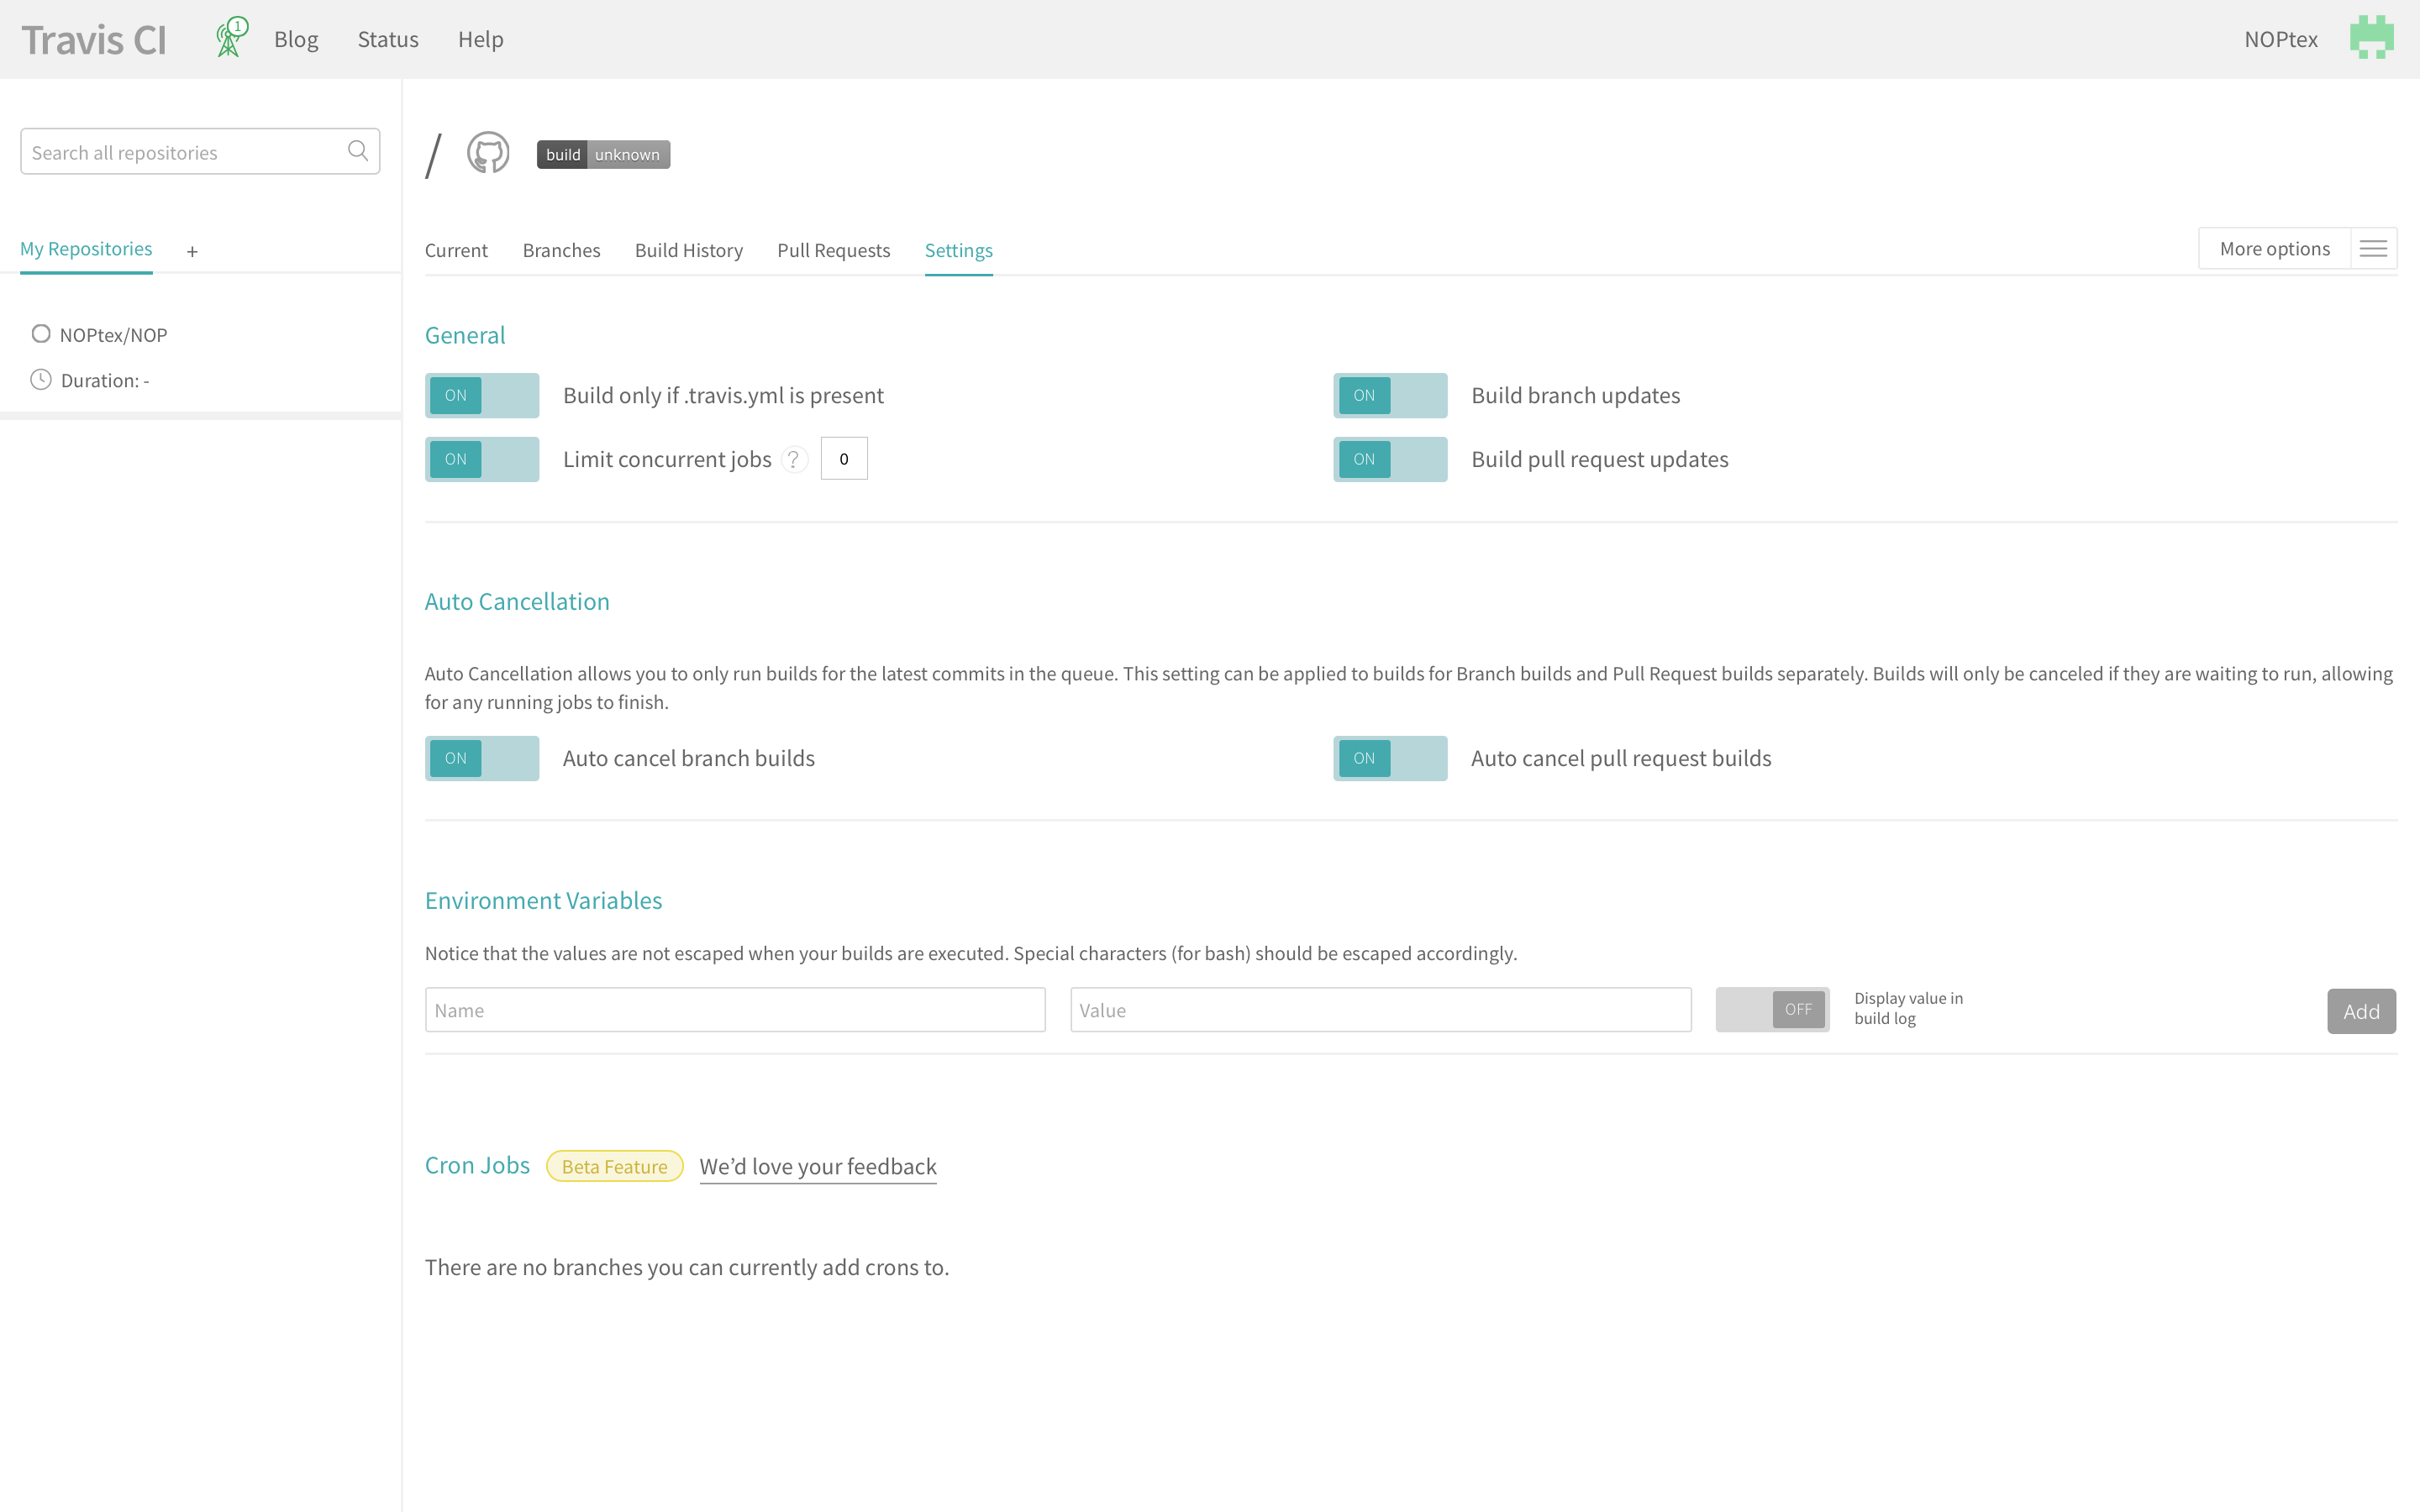
\includegraphics[width=1.0\textwidth]{./bilder/8TRAVISOptionsSET.png}
\end{framed}

\end{minipage}}
\hfill
\adjustbox{valign=t}{\begin{minipage}[t]{0.45\textwidth}
\vspace{0pt}
\huge
Ich setze alle Häkchen weil:
\begin{itemize}
  \item nur releases Gebaut werden sollen \\ (Testen kann man lokal) \\ Alle anderen Build sollen abgebrochen werden.
  \item Nur wenn .travis.yml vorhanden ist Build starten. \\(Einfaches deaktivieren über Git)
\end{itemize}
% \caption{Kapazität}
\end{minipage}}
\end{figure}

\clearpage % GleitObjekte anzeigen


%
% \newpage % ============================================= Newpage ===================
%
%
% \begin{figure}[ht]
%   \subsubsection{Build-Einstellungen setzen}
% \adjustbox{valign=t}{\begin{minipage}[t]{0.50\textwidth}
% \begin{framed}
%   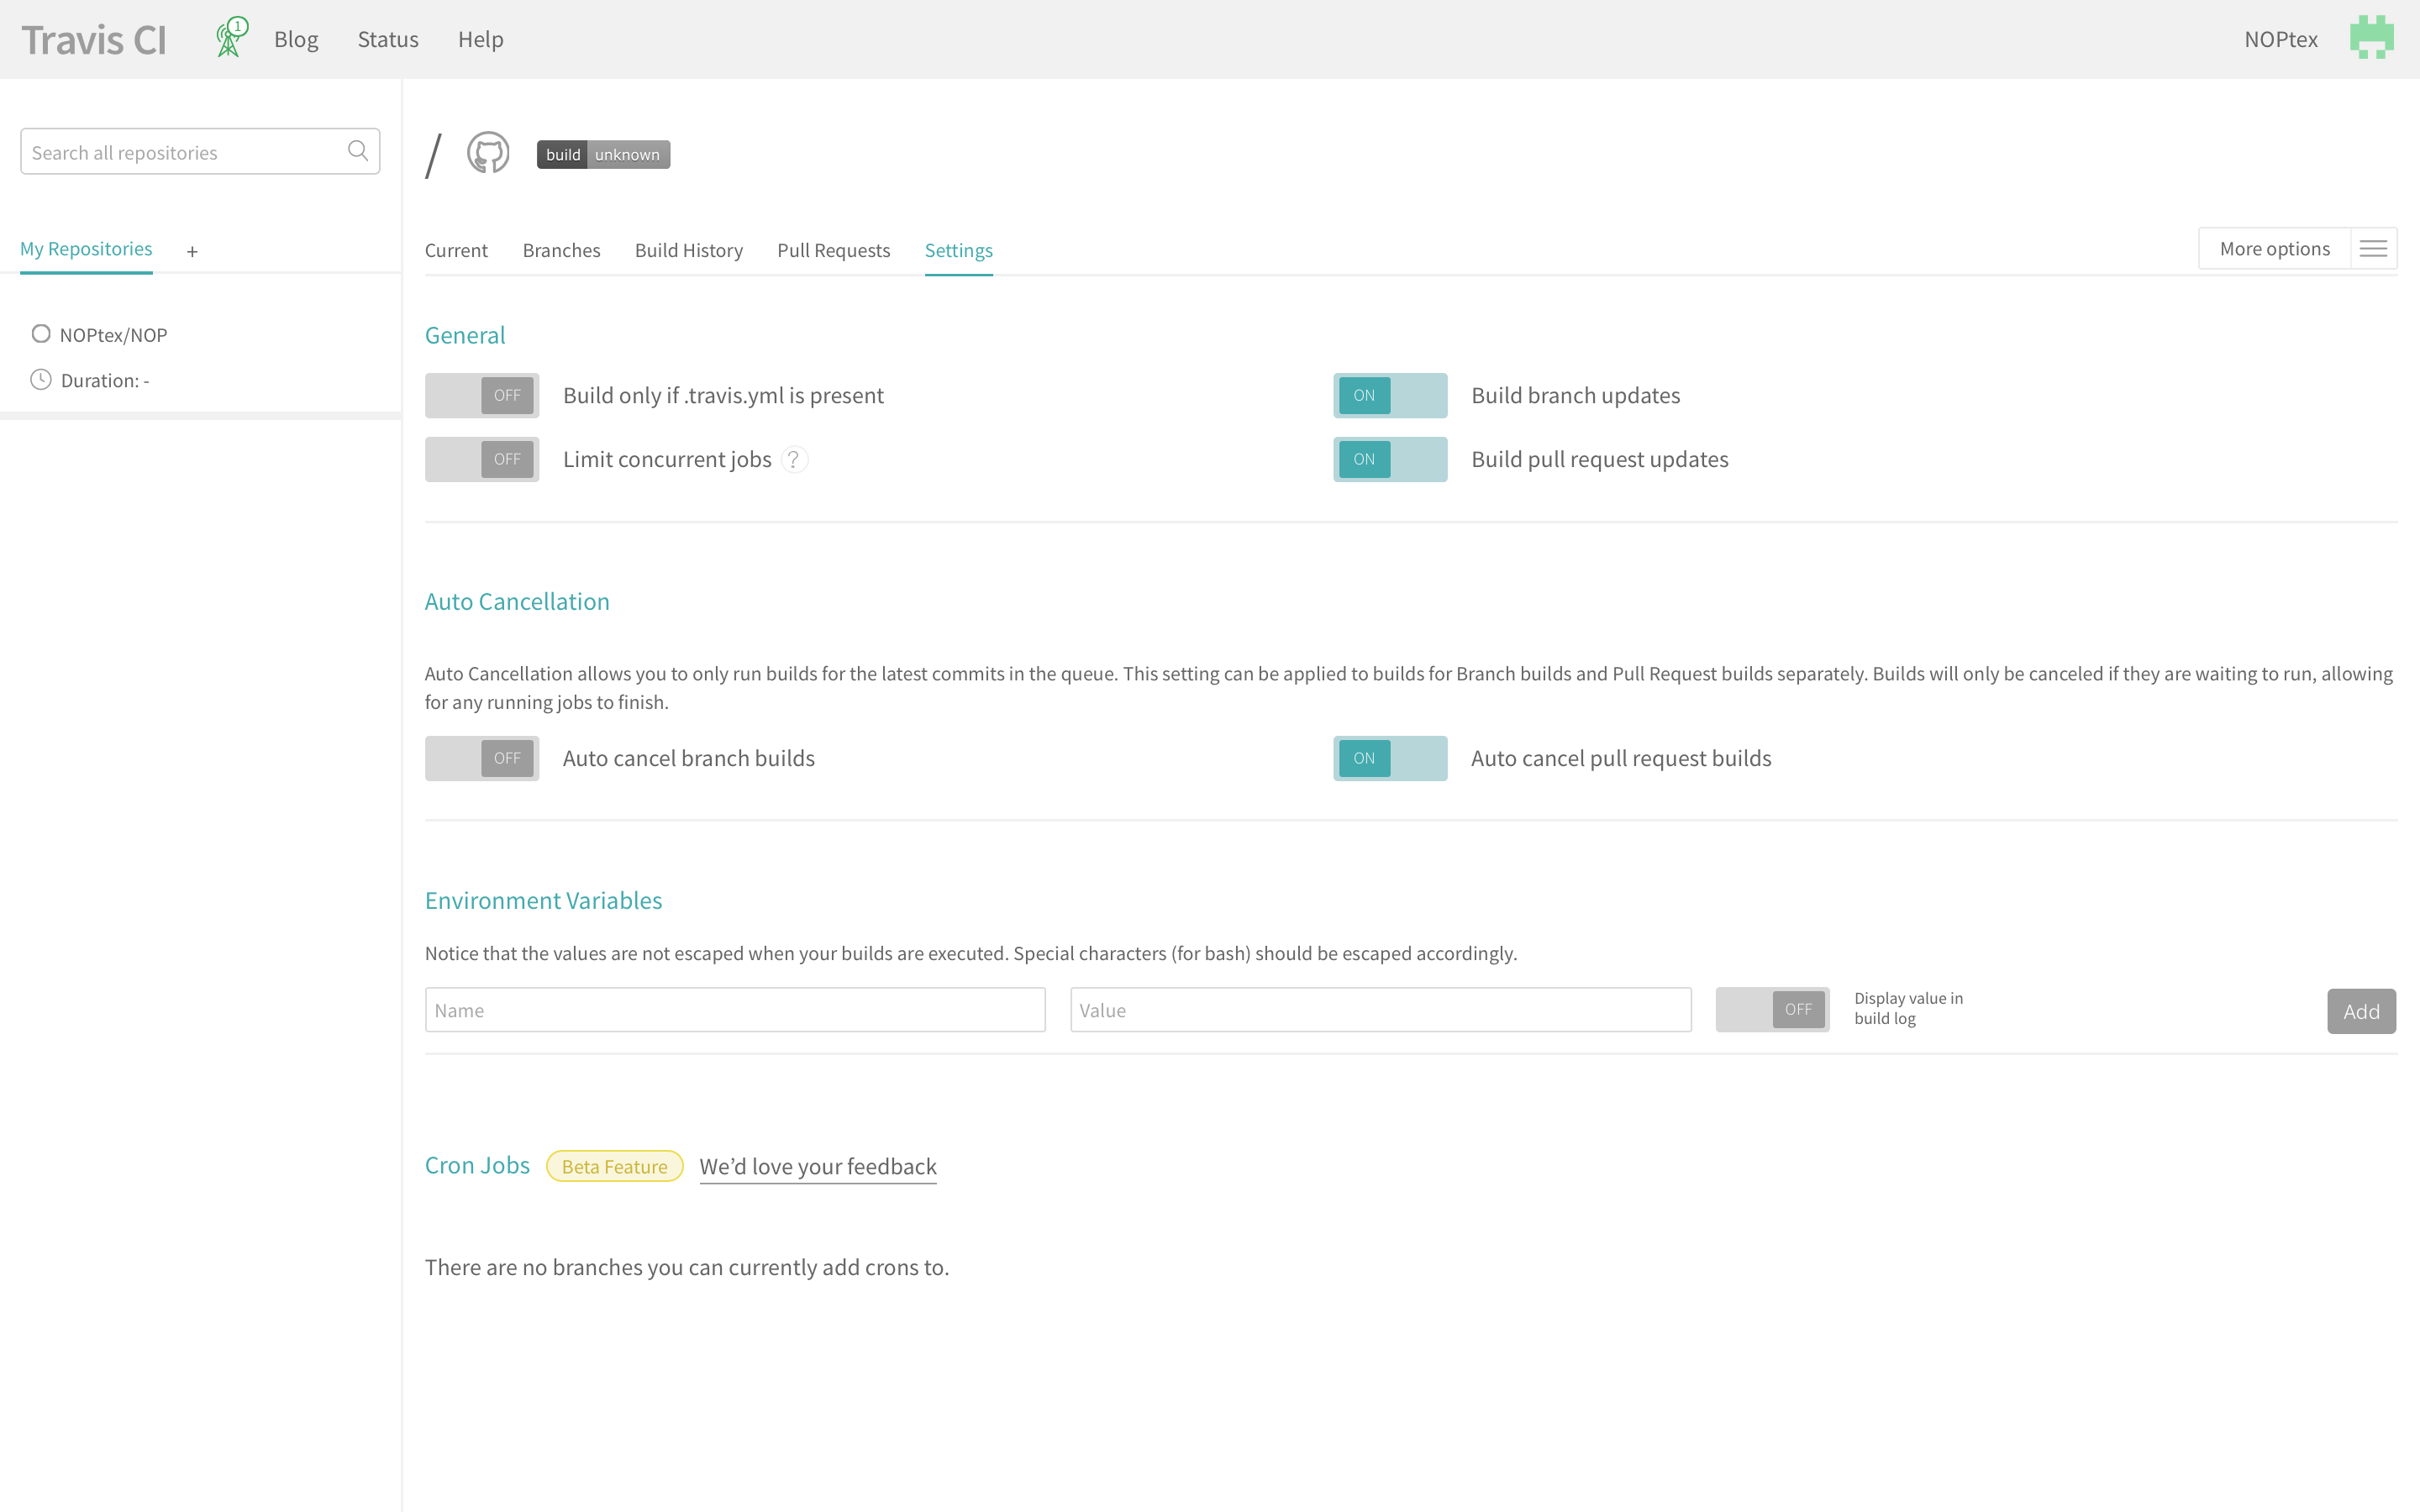
\includegraphics[width=1.0\textwidth]{./bilder/7TRAVISOptionsbase.png}
% \end{framed}
%
% \end{minipage}}
% % \hfill
% \adjustbox{valign=t}{\begin{minipage}[t]{0.45\textwidth}
% \vspace{0pt}
% 
\includegraphics[width=1.0\textwidth]{./bilder/7_1REPOsettings.png}
% \huge
% Über das Zahnrad kommt man zu den Einstellungen.
% % \caption{Kapazität}
% \end{minipage}}
% % \end{figure}
% % \vspace{0.5cm} % ----------------------------------- vspace
% % \begin{figure}[ht]
% \adjustbox{valign=t}{\begin{minipage}[t]{0.50\textwidth}
% % \vspace{0.5cm}
% \begin{framed}
%   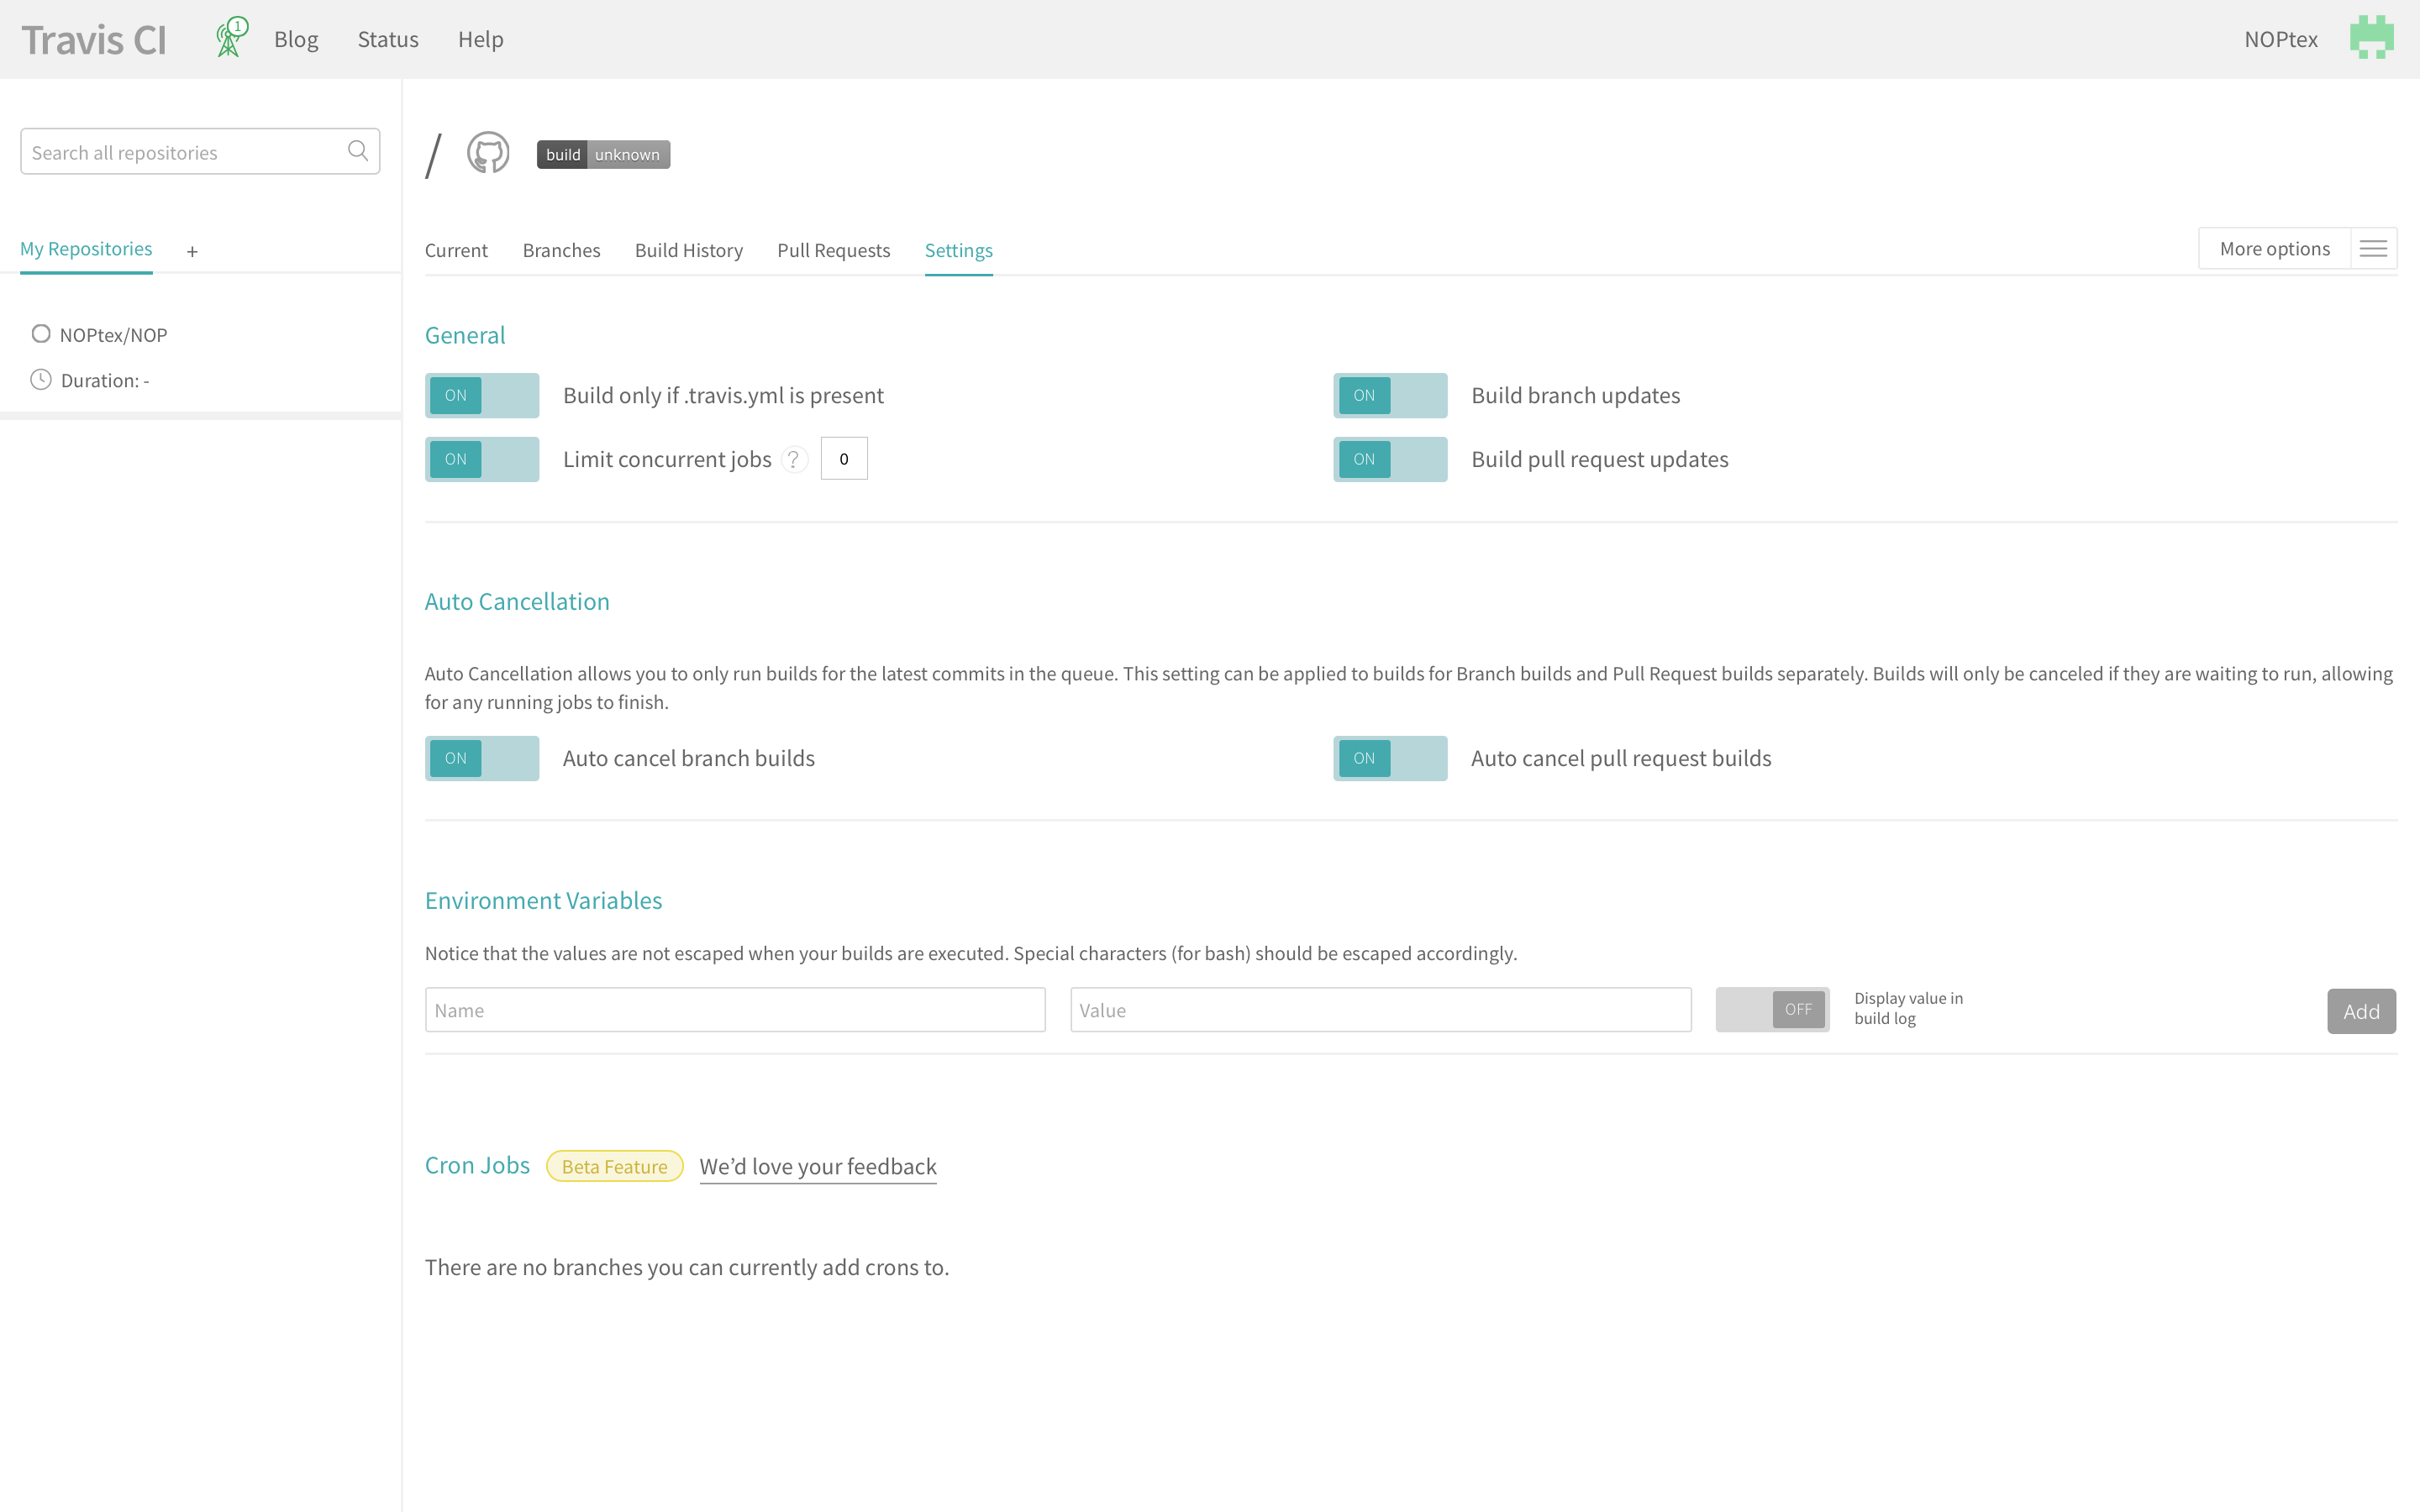
\includegraphics[width=1.0\textwidth]{./bilder/8TRAVISOptionsSET.png}
% \end{framed}
%
% \end{minipage}}
% \hfill
% \adjustbox{valign=t}{\begin{minipage}[t]{0.45\textwidth}
% \vspace{0pt}
% \huge
% Ich setze alle Häkchen weil:
% \begin{itemize}
%   \item nur releases Gebaut werden sollen \\ (Testen kann man lokal) \\ Alle anderen Build sollen abgebrochen werden.
%   \item Nur wenn .travis.yml vorhanden ist Build starten. \\(Einfaches deaktivieren über Git)
% \end{itemize}
% % \caption{Kapazität}
% \end{minipage}}
% \end{figure}
%
% \clearpage % GleitObjekte anzeigen




% \input{dummy.tex}
% \input{dummy.tex}
% \input{dummy.tex}
% \input{dummy.tex}

% \input{prog1.tex}



%  die beiden unteren beiden includen

% \input{kap1_vorl.tex}
% \input{kap2_vorl.tex}
% \input{kap3_vorl.tex}
% \input{kap4_vorl.tex}
% \input{kap5_vorl.tex}
% \input{kap6_vorl.tex}
% kapitel 7 im Buch

%   Kapitel 2

% \input{2ndKap7.tex}




%==============================================

% % programmieren 2

% \input{kap8.tex}
% \input{kap9.tex}
% \input{kap10.tex}
% \input{kap11.tex}
% \input{kap12.tex}
% \input{last.tex}
% \input{einfuerung.tex}




%=========================================================================================================================
%
%-------------END
\end{document}
